\documentclass[10pt]{jsarticle}%文字サイズが10ptのjsarticle

%%%%%%%%%%%%%%%%%%%%%%%%%%%%%%%%%%%%%%%%%%%%%%%%%%%%%%%
%%  パッケージ                                        %%
%%%%%%%%%%%%%%%%%%%%%%%%%%%%%%%%%%%%%%%%%%%%%%%%%%%%%%%
%使用しないときはコメントアウトしてください
\usepackage{amsthm}%定理環境
\usepackage{framed}%文章を箱で囲う
\usepackage{amsmath,amssymb}%数式全般
\usepackage[dvipdfmx]{graphicx}%図の挿入
%\usepackage{tikz}%描画
\usepackage{titlesec}%見出しの見た目を編集できる
\usepackage[dvipdfmx, usenames]{color}%色をつける
%\usepackage{tikz-cd}%可換図式
%\usepackage{mathtools}%数式関連
\usepackage{amsfonts}%数式のフォント
\usepackage[all]{xy}%可換図式
\usepackage{mathrsfs}%花文字
\usepackage{comment}%コメント環境
\usepackage{picture}%お絵かき
\usepackage{url}%URLを出力
\usepackage[dvipdfmx]{hyperref}
\usepackage{pxjahyper}%日本語しおりの文字化けを防ぐ

%%%%%%%%%%%%%%%%%%%%%%%%%%%%%%%%%%%%%%%%%%%%%%%%%%%%%%%
%%  表紙                                             %%
%%%%%%%%%%%%%%%%%%%%%%%%%%%%%%%%%%%%%%%%%%%%%%%%%%%%%%%
\makeatletter
\def\thickhrulefill{\leavevmode \leaders \hrule height 1pt\hfill \kern \z@}
\renewcommand{\maketitle}{\begin{titlepage}%
    \let\footnotesize\small
    \let\footnoterule\relax
    \parindent \z@
    \reset@font
    \null\vfil
    \begin{flushleft}
      \huge \@title
    \end{flushleft}
    \par
    \hrule height 4pt
    \par
    \begin{flushright}
      \LARGE \@author \par
    \end{flushright}
    \vskip 60\p@
    \vfil\null
    \begin{flushright}
        {\small \@date}%
    \end{flushright}
  \end{titlepage}%
  \setcounter{footnote}{0}%
}
\makeatother

%%%%%%%%%%%%%%%%%%%%%%%%%%%%%%%%%%%%%%%%%%%%%%%%%%%%%%%
%%  sectionの修飾                                     %%
%%%%%%%%%%%%%%%%%%%%%%%%%%%%%%%%%%%%%%%%%%%%%%%%%%%%%%%
\titleformat{\section}[block]
{}{}{0pt}
{
  \colorbox{black}{\begin{picture}(0,10)\end{picture}}
  \hspace{0pt}
  \normalfont \Large\bfseries
  \hspace{-4pt}
}
[
\begin{picture}(100,0)
  \put(3,18){\color{black}\line(1,0){300}}
\end{picture}
\\
\vspace{-30pt}
]

%%%%%%%%%%%%%%%%%%%%%%%%%%%%%%%%%%%%%%%%%%%%%%%%%%%%%%%
%%  太字section                                     %%
%%%%%%%%%%%%%%%%%%%%%%%%%%%%%%%%%%%%%%%%%%%%%%%%%%%%%%%
\newcommand{\bfsubsection}[1]{\subsection*{\textbf{#1}}}
\newcommand{\bfsection}[1]{\section*{\textbf{#1}}}

%%%%%%%%%%%%%%%%%%%%%%%%%%%%%%%%%%%%%%%%%%%%%%%%%%%%%%%
%%  番号付き定理環境                                  %%
%%%%%%%%%%%%%%%%%%%%%%%%%%%%%%%%%%%%%%%%%%%%%%%%%%%%%%%
%注:defというコマンドはもうある
\theoremstyle{definition}%定理環境のアルファベットを斜体にしない
\renewcommand{\proofname}{\textgt{証明}}%proof環境の修正

%%%%%%%%%%%%%%%%%%%%%%%%%%%%%%%%%%%%%%%%%%%%%%%%%%%%%%%
%%  番号なし定理環境                                  %%
%%%%%%%%%%%%%%%%%%%%%%%%%%%%%%%%%%%%%%%%%%%%%%%%%%%%%%%
%一部箱付き
\newtheorem*{lemma}{補題}
\newtheorem*{proposition}{命題}
\newtheorem*{definition}{定義}
\newcommand{\lem}[1]{\begin{oframed} \begin{lemma} #1 \end{lemma} \end{oframed}}%箱付きほだい
\newcommand{\prop}[1]{\begin{oframed} \begin{proposition} #1 \end{proposition} \end{oframed}}%箱付きめいだい

\newtheorem*{claim}{主張}
\newtheorem*{sol}{解答}
\newtheorem*{prob}{問題}
\newtheorem*{quo}{引用}
\newtheorem*{rem}{注意}



%%%%%%%%%%%%%%%%%%%%%%%%%%%%%%%%%%%%%%%%%%%%%%%%%%%%%%%
%%  左側に線を引く                                  %%
%%%%%%%%%%%%%%%%%%%%%%%%%%%%%%%%%%%%%%%%%%%%%%%%%%%%%%%
%leftbar環境の定義
\makeatletter
\renewenvironment{leftbar}{%
%  \def\FrameCommand{\vrule width 3pt \hspace{10pt}}%  デフォルトの線の太さは3pt
  \renewcommand\FrameCommand{\vrule width 1pt \hspace{10pt}}%
  \MakeFramed {\advance\hsize-\width \FrameRestore}}%
 {\endMakeFramed}
\newcommand{\exbf}[2]{ \begin{leftbar} \textbf{#1} #2 \end{leftbar} }%左線つき太字
%\newcommand{\barquo}[1]{\begin{leftbar} \begin{quo} #1 \end{quo} \end{leftbar}}%左線つき引用%びふぉあ
\newcommand{\barquo}[1]{\begin{leftbar} \noindent #1  \end{leftbar}}%左線つき引用%あふたー
\newcommand{\lbar}[1]{\begin{leftbar} #1 \end{leftbar}}



%%%%%%%%%%%%%%%%%%%%%%%%%%%%%%%%%%%%%%%%%%%%%%%%%%%%%%%
%%  色をつける                                      %%
%%%%%%%%%%%%%%%%%%%%%%%%%%%%%%%%%%%%%%%%%%%%%%%%%%%%%%%
\newcommand{\textblue}[1]{\textcolor{blue}{\textbf{#1}}}

%%%%%%%%%%%%%%%%%%%%%%%%%%%%%%%%%%%%%%%%%%%%%%%%%%%%%%%
%%  よく使う記号の略記                                 %%
%%%%%%%%%%%%%%%%%%%%%%%%%%%%%%%%%%%%%%%%%%%%%%%%%%%%%%%
\newcommand{\setmid}[2]{\left\{ #1 \mathrel{} \middle| \mathrel{} #2 \right\}}%集合の内包記法
\newcommand{\sm}{\setminus}%集合差
\newcommand{\abs}[1]{\left \lvert #1 \right \rvert}%絶対値
\newcommand{\norm}[1]{\left \lVert #1 \right \rVert}%ノルム
\newcommand{\transpose}[1]{\, {\vphantom{#1}}^t\!{#1}}%行列の転置
\newcommand{\pmat}[1]{ \begin{pmatrix} #1 \end{pmatrix} }%まるかっこ行列
\newcommand{\f}[2]{\frac{#1}{#2}}%分数
\newcommand{\kakko}[1]{ \langle #1  \rangle}%鋭角かっこ%\angleはもうある
\newcommand{\I}{\sqrt{-1}}%虚数単位。\iは既にある。
\newcommand{\single}{\{ 0 \}}%0のシングルトン
\newcommand{\clsub}{\subset_{\text{closed}}}%閉部分集合
\newcommand{\opsub}{\subset_{\text{open}}}%開部分集合
\newcommand{\clirr}{\subset_{\text{closed irr}}}%閉既約部分集合
\newcommand{\loc}{\subset_{\text{loc. closed}}}%局所閉部分集合
\newcommand{\wt}[1]{\widetilde{#1}}%わいどちるだあ
\newcommand{\ol}[1]{\overline{#1}}%オーバーライン
\newcommand{\wh}[1]{\widehat{#1}}%ワイドハット
\newcommand{\To}{\Rightarrow}%ならば%自然変換
\newcommand{\xto}[1]{\xrightarrow}%上側文字付き右向き矢印
\newcommand{\st}{\; \; \text{s.t.} \; \;}%空白付きsuch that
\newcommand{\ts}{\otimes}%テンソル積
\newcommand{\tm}{\times}%直積
\newcommand{\vartm}{\times^{\text{Var}}}%多様体の圏における直積。集合の直積と区別するとき用。
\newcommand{\la}{\overleftarrow}%上付き左矢印
\newcommand{\ra}{\overrightarrow}%上付き右矢印
\newcommand{\del}{\partial}%偏微分の記号



%%%%%%%%%%%%%%%%%%%%%%%%%%%%%%%%%%%%%%%%%%%%%%%%%%%%%%%
%%       演算子                                       %%
%%%%%%%%%%%%%%%%%%%%%%%%%%%%%%%%%%%%%%%%%%%%%%%%%%%%%%%
%log型
\DeclareMathOperator{\rank}{rank}%行列の階数
\DeclareMathOperator{\rk}{rk}%行列の階数
\DeclareMathOperator{\corank}{corank}%行列の核の次元
\renewcommand{\Re}{\operatorname{Re}}%実部
\DeclareMathOperator{\Res}{Res}%留数
\DeclareMathOperator{\Gal}{Gal}%Galois群
\DeclareMathOperator{\Hom}{Hom}%射の集合
\DeclareMathOperator{\ind}{Ind}
\DeclareMathOperator{\tr}{Trace}%トレース
\DeclareMathOperator{\Aut}{Aut}%自己同型群
\DeclareMathOperator{\trdeg}{tr\text{.}deg}%超越次数
\DeclareMathOperator{\Frac}{Frac}%商体をとる操作
\renewcommand{\Im}{\operatorname{Im}}%写像の像。Abel圏の像対象。虚部が出力できなくなった。
\DeclareMathOperator{\Ker}{Ker}%写像の核。Abel圏の核対象。
\DeclareMathOperator{\im}{im}%写像の像
\DeclareMathOperator{\coker}{coker}%余核%対象のほう
\DeclareMathOperator{\Coker}{Coker}%余核%射のほう
\DeclareMathOperator{\Spec}{Spec}%スペクトル
\DeclareMathOperator{\Sing}{Sing}%Singular point.特異点の集合。歌ってるわけではないぞ
\DeclareMathOperator{\Supp}{Supp}%台
\DeclareMathOperator{\ann}{ann}%アナイアレーター
\DeclareMathOperator{\Ass}{Ass}%素因子
\DeclareMathOperator{\ord}{ord}%おーだー
\DeclareMathOperator{\height}{ht}%素イデアルの高度。\htはもうある
\DeclareMathOperator{\coht}{coht}%素イデアルの余高度
\DeclareMathOperator{\Lan}{Lan}%左Kan拡張
\DeclareMathOperator{\Ran}{Ran}%右Kan拡張



%limit型
\DeclareMathOperator*{\llim}{\varprojlim}%極限。逆極限。射影極限。
\DeclareMathOperator*{\rlim}{\varinjlim}%余極限。順極限。入射極限。

%%%%%%%%%%%%%%%%%%%%%%%%%%%%%%%%%%%%%%%%%%%%%%%%%%%%%%%
%%  黒板太字(blackboard bold)                         %%
%%%%%%%%%%%%%%%%%%%%%%%%%%%%%%%%%%%%%%%%%%%%%%%%%%%%%%%
\newcommand{\bba}{{\mathbb A}}
\newcommand{\bbb}{{\mathbb B}}
\newcommand{\bbc}{{\mathbb C}}
\newcommand{\bbd}{{\mathbb D}}
\newcommand{\bbe}{{\mathbb E}}
\newcommand{\bbf}{{\mathbb F}}
\newcommand{\bbg}{{\mathbb G}}
\newcommand{\bbh}{{\mathbb H}}
\newcommand{\bbi}{{\mathbb I}}
\newcommand{\bbj}{{\mathbb J}}
\newcommand{\bbk}{{\mathbb K}}
\newcommand{\bbl}{{\mathbb L}}
\newcommand{\bbm}{{\mathbb M}}
\newcommand{\bbn}{{\mathbb N}}
\newcommand{\bbo}{{\mathbb O}}
\newcommand{\bbp}{{\mathbb P}}
\newcommand{\bbq}{{\mathbb Q}}
\newcommand{\bbr}{{\mathbb R}}
\newcommand{\bbs}{{\mathbb S}}
\newcommand{\bbt}{{\mathbb T}}
\newcommand{\bbu}{{\mathbb U}}
\newcommand{\bbv}{{\mathbb V}}
\newcommand{\bbw}{{\mathbb W}}
\newcommand{\bbx}{{\mathbb X}}
\newcommand{\bby}{{\mathbb Y}}
\newcommand{\bbz}{{\mathbb Z}}

%%%%%%%%%%%%%%%%%%%%%%%%%%%%%%%%%%%%%%%%%%%%%%%%%%%%%%%
%%  よく使う黒板太字                                  %%
%%%%%%%%%%%%%%%%%%%%%%%%%%%%%%%%%%%%%%%%%%%%%%%%%%%%%%%
\newcommand{\Z}{\bbz}
\newcommand{\A}{\bba}
\newcommand{\Q}{\bbq}
\newcommand{\R}{\bbr}
\newcommand{\C}{\bbc}
\newcommand{\F}{\bbf}
\newcommand{\N}{\bbn}
\renewcommand{\P}{\bbp}%パラグラフ記号が出力できなくなった

%%%%%%%%%%%%%%%%%%%%%%%%%%%%%%%%%%%%%%%%%%%%%%%%%%%%%%%
%%  カリグラフィー                                %%
%%%%%%%%%%%%%%%%%%%%%%%%%%%%%%%%%%%%%%%%%%%%%%%%%%%%%%%
%大文字しかどうせ使わない
\newcommand{\cala}{\mathcal{A}}
\newcommand{\calb}{\mathcal{B}}
\newcommand{\calc}{\mathcal{C}}
\newcommand{\cald}{\mathcal{D}}
\newcommand{\calf}{\mathcal{F}}
\newcommand{\calo}{\mathcal{O}}

%%%%%%%%%%%%%%%%%%%%%%%%%%%%%%%%%%%%%%%%%%%%%%%%%%%%%%%
%%  ギリシャ文字(Greek letters)小文字                 %%
%%%%%%%%%%%%%%%%%%%%%%%%%%%%%%%%%%%%%%%%%%%%%%%%%%%%%%%
%コマンドが5字以上のもの
\newcommand{\gra}{{\alpha}}
\newcommand{\grg}{{\gamma}}
\newcommand{\grd}{{\delta}}
\newcommand{\gre}{{\epsilon}}
\newcommand{\grt}{{\theta}}
\newcommand{\grk}{{\kappa}}
\newcommand{\grl}{{\lambda}}
\newcommand{\grs}{{\sigma}}
\newcommand{\gru}{{\upsilon}}
\newcommand{\gro}{{\omega}}

\newcommand{\ve}{{\varepsilon}}
\newcommand{\vp}{{\varphi}}

%%%%%%%%%%%%%%%%%%%%%%%%%%%%%%%%%%%%%%%%%%%%%%%%%%%%%%%
%%  ギリシャ文字(Greek letters)大文字                 %%
%%%%%%%%%%%%%%%%%%%%%%%%%%%%%%%%%%%%%%%%%%%%%%%%%%%%%%%
%コマンドが5字以上のもの
\newcommand{\grG}{{\Gamma}}
\newcommand{\grD}{{\Delta}}
\newcommand{\grT}{{\Theta}}
\newcommand{\grL}{{\Lambda}}
\newcommand{\grS}{{\Sigma}}
\newcommand{\grU}{{\Upsilon}}
\newcommand{\grO}{{\Omega}}

%%%%%%%%%%%%%%%%%%%%%%%%%%%%%%%%%%%%%%%%%%%%%%%%%%%%%%%
%%  フラクトゥール                                  %%
%%%%%%%%%%%%%%%%%%%%%%%%%%%%%%%%%%%%%%%%%%%%%%%%%%%%%%%
\newcommand{\fraka}{\mathfrak{a}}
\newcommand{\frakb}{\mathfrak{b}}
\newcommand{\frakm}{\mathfrak{m}}
\newcommand{\frakp}{\mathfrak{p}}

\newcommand{\frakA}{\mathfrak{A}}
\newcommand{\frakB}{\mathfrak{B}}
\newcommand{\frakT}{\mathfrak{T}}

\newcommand{\Top}{\mathfrak{Top}}%開部分集合全体のなす有向集合
\newcommand{\Ab}{\mathfrak{Ab}}%Abel群のなす圏

%%%%%%%%%%%%%%%%%%%%%%%%%%%%%%%%%%%%%%%%%%%%%%%%%%%%%%%
%%  花文字                                          %%
%%%%%%%%%%%%%%%%%%%%%%%%%%%%%%%%%%%%%%%%%%%%%%%%%%%%%%%
%大文字しかどうせ使わない
\newcommand{\scra}{\mathscr{A}}
\newcommand{\scrf}{\mathscr{F}}
\newcommand{\scrg}{\mathscr{G}}
\newcommand{\scrh}{\mathscr{H}}
\newcommand{\scrs}{\mathscr{S}}

%%%%%%%%%%%%%%%%%%%%%%%%%%%%%%%%%%%%%%%%%%%%%%%%%%%%%%%
%%  太字                                            %%
%%%%%%%%%%%%%%%%%%%%%%%%%%%%%%%%%%%%%%%%%%%%%%%%%%%%%%%
\newcommand{\Sh}{\textbf{Sh}}%層の圏
\newcommand{\PSh}{\textbf{PSh}}%前層の圏
\newcommand{\bfzero}{\textbf{0}}%太字のゼロ

%小文字
\newcommand{\bfb}{\textbf{b}}
\newcommand{\bfv}{\textbf{v}}
\newcommand{\bfx}{\textbf{x}}
\newcommand{\bfy}{\textbf{y}}


%大文字
\newcommand{\bfC}{\textbf{C}}
\newcommand{\bfD}{\textbf{D}}
\newcommand{\bfE}{\textbf{E}}



\setcounter{tocdepth}{3}%目次に含めるレベル。1ならsectionまで。2ならsubsectionまで。3ならsubsubsectionまで。
\begin{document}



\title{京都大学数学・数理解析専攻院試過去問}
\author{北窓 \\ \url{https://seasawher.github.io/kitamado/} }
\date{\today}
\maketitle




\tableofcontents%目次
\newpage



\section{はじめに}

京都大学数学・数理解析専攻の院試の問題と解答です。問題文は\url{https://www.math.kyoto-u.ac.jp/ja/past-exams}から入手したものを使用しています。なおMicrosoft Edgeで閲覧することを推奨いたします。

この解答を作るにあたって、協力してくださった方々に感謝します。すむーずぷりんちゃん (@mat\_der\_D)氏には平成31年度基礎問4を解いていただきました。キヅ(@28Vittorio)さんと、ひろ(@azureh97)さんは院試ゼミのメンバーとして協力してくださいました。また、ナカトウ氏による解答も大変参考にさせていただきました。お礼申し上げます。また、私が難しい問題に悩んでいるときにいつも適切なアドバイスをくれたM君にこの場を借りて謝意を表します。

解答作成には万全を期しましたが、この解答を使用することにより使用者に不利益が生じたとしても、解答執筆者である私(北窓)は責任を負いません。したがって書かれていることが正しいかどうかはよくご自分で確認されるようにお願いします。とくに私(北窓)は計算間違いや救いようのない勘違いをよくするので。

このPDFのコピー・再配布を許可します。ただし再配布の際にも「コピー・再配布は自由」として下さい。加筆・改変は私(北窓)のGitHubアカウント(\url{https://github.com/Seasawher})を通してくださればと思います。


\newpage



\section{平成31年度 基礎科目}


\subsubsection{}

\barquo{
$\gra$は$0 < \gra < \f{\pi}{2}$を満たす定数とする。このとき広義積分
\[
\iint_D e^{-(x^2 + 2xy \cos \gra + y^2)} \ dx dy
\]
を計算せよ。ただし、$D=\setmid{(x,y) \in \R^2 }{ x \geq 0, y \geq 0}$とする。
}
\begin{sol}
$x = r \cos \grt$, $y = r \sin \grt$と変数変換する。領域$D$は、$\setmid{(r,\grt)}{r \geq 0, 0 \leq \grt \leq \f{\pi}{2} }$へ移る。すると$dx dy = r dr d\grt$であって
\begin{align*}
  \iint_D e^{-(x^2 + 2xy \cos \gra + y^2)} \ dx dy &= \int_0^{\f{\pi}{2}} \ d\grt \int_{0}^{\infty} e^{-r^2(1 + \sin 2 \grt \cos \gra)} r \ dr \\
  &= \f{1}{2} \int_0^{\f{\pi}{2}} \ d\grt \int_{0}^{\infty} e^{-r(1 + \sin 2 \grt \cos \gra)}  \ dr \\
  &= \f{1}{2} \int_0^{\f{\pi}{2}} \f{d \grt}{1 + \sin 2\grt \cos \gra} \\
  &= \f{1}{4} \int_0^{\pi} \f{d \grt}{1 + \sin \grt \cos \gra}
\end{align*}
と計算できる。さらに$t = \tan \f{\grt}{2}$として変数変換を行う。$d\grt = 2(1+t^2)^{-1} dt$で、$\sin \grt = 2t / (1+t^2)$だから
\begin{align*}
    \iint_D e^{-(x^2 + 2xy \cos \gra + y^2)} \ dx dy &= \f{1}{4} \int_0^{\infty} \f{2(1+t^2)^{-1} dt}{1 + 2t(1+t^2)^{-1}  \cos \gra} \\
    &= \f{1}{2} \int_0^{\infty} \f{dt}{(t+ \cos \gra)^2 + \sin^2 \gra } \\
    &= \f{1}{2} \int_{\cos \gra}^{\infty} \f{dt}{t^2 + \sin^2 \gra } \\
    &= \f{1}{2 \sin \gra} \int_{1 / \tan \gra}^{\infty} \f{dt}{t^2 + 1} \\
    &= \f{1}{2 \sin \gra} \left( \f{\pi}{2} - \arctan \left( \f{1}{\tan \gra} \right) \right)
\end{align*}
である。ここで、$\tan(\f{\pi}{2} - \gra ) = \f{1}{\tan \gra}$であることから、結論として次を得る。
\[
\iint_D e^{-(x^2 + 2xy \cos \gra + y^2)} \ dx dy = \f{\gra}{2 \sin \gra}
\]
\end{sol}


\newpage


\subsubsection{}
\barquo{
複素数$\gra$に対し、3次複素正方行列$A(\gra)$を次のように定める。
\[
A(\gra) = \pmat{ \gra -4 & \gra +4 & -2 \gra +1 \\ -2 & 2 \gra +1 & -2 \gra +2 \\ -1 & \gra & - \gra +2}
\]
\begin{description}
  \item[(1)] $A(\gra)$の行列式を求めよ。
  \item[(2)] $A(\gra)$の階数を求めよ。
\end{description}
}
\begin{sol} ${}$
\begin{description}
  \item[(1)] ある行に別の行の定数倍を足す操作を繰り返し行っていくと
  \begin{align*}
    A(\gra) &\sim \pmat{ \gra -3 & 4 & - \gra -1 \\ 0 & 1  & -2 \\ -1 & \gra & - \gra +2} \\
    &\sim \pmat{ \gra -3 & 0 & - \gra +7 \\ 0 & 1  & -2 \\ -1 & 0 & \gra +2} \\
    &\sim \pmat{ 0 & 0 & (\gra - 1)^2 \\ 0 & 1  & -2 \\ -1 & 0 & \gra +2} \\
  \end{align*}
  と変形できる。よって$\det A(\gra) = (\gra - 1)^2$である。
  \item[(2)] $\gra=1$のときは階数2である。それ以外のときは正則で、階数は3である。
\end{description}

\end{sol}


\newpage



\subsubsection{}
\barquo{
$(x_0, y_0) \in \R^2 \sm \{(0,0)\}$に対して、$\R$上の連立常微分方程式
\[
\begin{cases}
  \f{dx}{dt} = -x^2 y - y^3 \\
    \f{dy}{dt} = x^3 +  xy^2
\end{cases}
\quad
\begin{cases}
x(0) = x_0 \\
y(0) = y_0
\end{cases}
\]
の解$(x(t),y(t))$は周期を持つことを示し、最小の周期を求めよ。ただし正の実数$T$が$(x(t),y(t))$の周期であるとは、任意の$t \in \R$に対して
\[
(x(t + T),y(t + T)) = (x(t),y(t))
\]
が成り立つことである。
}
\begin{sol}
与式より
\begin{align*}
  x \f{dx}{dt} + y \f{dy}{dt} &= 0 \\
  \f{d}{dt}(x^2 + y^2) &= 0
\end{align*}
を得る。したがって$C = x^2 + y^2$は定数であり、$C = x_0^2 + y_0^2$が成り立つ。ゆえに与式は
\[
\begin{cases}
  \f{dx}{dt} = - Cy \\
    \f{dy}{dt} = Cx
\end{cases}
\]
と書き直せる。この連立方程式を一変数にまとめると
\[
\f{d^2 x}{dt^2} = - C^2 x
\]
となるが、この解空間は$\cos (C t)$と$\sin (Ct)$で張られる。したがって、一般解はこの線形結合で書けるのだから
\begin{align*}
  x(t) = x_0 \cos(Ct) - y_0 \sin (Ct) \\
  y(t) = y_0 \cos(Ct) + x_0 \sin (Ct)
\end{align*}
でなくてはならない。常微分方程式の初期値問題の解の一意性より、解はこれだけである。よって求める周期は$2\pi / C$である。
\end{sol}

\newpage


\subsubsection{}
\barquo{
$f$は$\R$上の実数値$C^1$級関数で任意の$x \in \R$に対して$f(x+1)=f(x)$を満たすとする。このとき以下の2条件は同値であることを示せ。
\begin{description}
  \item[(A)] 広義積分
  \[
  \int_1^{\infty} \f{1}{x^{1+f(x)^2}} \ dx
  \]
  が収束する。
  \item[(B)] $f(x) = 0$となる$x \in \R$が存在しない。
\end{description}
}
\begin{sol} ${}$
  \begin{description}
    \item[(B)$\To$(A)] このときある$\ve > 0$が存在して$\forall x \; f(x)^2 > \ve$が成り立つ。よって
    \begin{align*}
            \int_1^{\infty} \f{1}{x^{1+f(x)^2}} \ dx \leq \int_1^{\infty} \f{dx}{x^{1+\ve}}
            \leq \f{1}{\ve}
    \end{align*}
    より積分は有界である。被積分関数は正の値しかとらないので、これで広義積分の収束がいえた。
    \item[(A)$\To$(B)] 対偶を示そう。$f(a)=0$なる$a$があったとする。周期性から$f(a_1)=0$なる$1 \leq a_1 < 2$がとれる。$n \geq 2$に対し$ n \leq a_n < n+1$を$a_n = a_1 + n-1$で定める。$f(x)=f(x+1)$より、$f$はコンパクト空間$\R / \Z$上の$C^1$級関数である。
    とくに$f'$は有界であり、$\forall x \; \abs{f'(x)} \leq M$なる$M > 0$をとることができる。したがって平均値の定理を適用することにより、任意の$n$について
    \[
    \abs{f(x)} = \abs{f(x) - f(a_n)} \leq M \abs{x - a_n}
    \]
    が成り立つことがわかる。ここまでの議論を踏まえると次の補題が示せる。
\lem{
ある$r > 0$が存在して、任意の自然数$n \geq 2$に対して
\[
\int_{2n-2}^{2n} x^{-f(x)^2} \ dx \geq \f{r}{ \sqrt{\log 2n} }
\]
が成り立つ。
}
\begin{proof}
  以下のように計算できる。
  \begin{align*}
    \int_{2n-2}^{2n} x^{-f(x)^2} \ dx  &\geq \int_{2n-2}^{2n} \exp \left\{ - (\log x) f(x)^2 \right\} \ dx \\
    &\geq \int_{2n-2}^{2n} \exp \left\{ - (\log 2n) f(x)^2 \right\} \ dx \\
  &\geq \int_{a_{2n-2}}^{a_{2n-2}+1} \exp \left\{ - (\log 2n) f(x)^2 \right\} \ dx \\
  &\geq \int_{a_{2n-2}}^{a_{2n-2}+1} \exp \left\{ - M^2(\log 2n) (x-a_{2n-2})^2 \right\} \ dx \\
  &\geq \int_{a_{2n-2}}^{a_{2n-2}+1} \exp \left\{ - (M \sqrt{\log 2n} (x-a_{2n-2}) )^2 \right\} \ dx
\end{align*}
変数変換$y=M \sqrt{\log 2n}(x-a_{2n-2})$を行って
\begin{align*}
 \int_{2n-2}^{2n} x^{-f(x)^2} \ dx  &\geq  \f{1}{M \sqrt{\log 2n}} \int_{0}^{M \sqrt{\log 2n} } e^{-y^2} \ dy  \\
  &\geq  \f{1}{M \sqrt{\log 2n}} \int_{0}^{M \sqrt{\log 4} } e^{-y^2} \ dy
  \end{align*}
  したがって
  \[
  r = \f{1}{M} \int_{0}^{M \sqrt{\log 4} } e^{-y^2} \ dy
  \]
  とおけばよい。
\end{proof}
(A)$\To$(B)の証明に戻る。$R \geq 4$に対し、$4 \leq 2N \leq R$を満たす最大の$N \in \Z$を$N_R$とおく。すると
\begin{align*}
  \int_1^R \f{dx}{x^{1+f(x)^2}} &\geq \sum_{n=2}^{N_R} \int_{2n-2}^{2n} \f{dx}{x^{1+f(x)^2}} \\
  &\geq \sum_{n=2}^{N_R} \f{1}{2n} \int_{2n-2}^{2n} \f{dx}{x^{f(x)^2}} \\
  &\geq \sum_{n=2}^{N_R} \f{r}{2n \sqrt{\log 2n}}
\end{align*}
というように評価できる。さらに$1/x\sqrt{\log x}$は単調減少なので
\begin{align*}
\int_1^R \f{dx}{x^{1+f(x)^2}} &\geq r \int_{2}^{N_R+1} \f{dx}{2x \sqrt{\log 2x}}  \\
&\geq \f{r}{2} \int_{4}^{2N_R+2} \f{dy}{y \sqrt{\log y}}  \\
&\geq r (\sqrt{\log(2N_R + 2)} - \sqrt{\log 4}) \\
&\geq r (\sqrt{R} - \sqrt{\log 4})
\end{align*}
である。ゆえに結論が従う。
  \end{description}
\end{sol}


\newpage

\subsubsection{} %\bfsubsection{問5}
\barquo{
$n$を2以上の整数、$A$を$n$次複素正方行列とする。$A^{n-1}$は対角化可能でないが、$A^n$が対角化可能であるとき、$A^n=0$となることを示せ。
}
\begin{sol}
$\C$係数なので、Jordan標準形が存在する。$A$ははじめからJordan標準形であるとしてよい。
\[
A = \bigoplus_{i=1}^r J_{\grl_i}(a_i)
\]
とする。$a_1, \cdots , a_r$は(異なるとは限らない)固有値であり、$\grl_i$はそれぞれのジョルダン細胞のサイズである。
\[
A^n = \bigoplus_{i=1}^r J_{\grl_i}(a_i)^n
\]
は対角化可能なので、各$J_{\grl_i}(a_i)^n$も対角化可能。ここで$J_{\grl_i}(a_i)$のJordan分解
\[
S_i = \pmat{a_i &  & &  \\  &  \ddots & &  \\ & & \ddots & \\ &  & & a_i} \quad N_i = \pmat{0 & 1 & & \\ & \ddots & \ddots & \\ & & \ddots & 1 \\ & & & 0 }
\]
を考える。
\[
J_{\grl_i}(a_i)^n = S_i^n + \sum_{k=1}^n \binom{n}{k} S_i^{n-k} N_i^k
\]
であって、$S_i^n$は対角行列で$\sum_{k=1}^n \binom{n}{k} S_i^{n-k} N_i^k$はべき零行列だから、Jordan分解の一意性より
\[
\sum_{k=1}^n \binom{n}{k} S_i^{n-k} N_i^k = 0
\]
を得る。左辺は具体的に書くことができて、次のような$\grl_i$次行列
\[
\pmat{
0 & \binom{n}{1} a_i^{n-1} & \binom{n}{2} a_i^{n-2} & \cdots & \binom{n}{\grl_i - 1} a_i \\
  & 0 & \binom{n}{1} a_i^{n-1} & \cdots & \binom{n}{\grl_i - 2} a_i^2 \\
  &   &  \ddots &  & \vdots \\
  &   &        &  &  0
}
\]
である。$\grl_i = 1$のときにはこの等式から情報を得ることはできない。しかし$\grl_i \geq 2$ならば$a_i = 0$であることがわかる。つまりサイズが$2$以上のJordan細胞はべき零である。実はサイズが$1$のJordan細胞は存在しない。ハイリホーで示す。仮に存在したとする。$n \geq 2$という仮定より、このときサイズが$2$以上のJordan細胞のサイズは$n-1$以下でなくてはならない。したがって、サイズが$2$以上のJordan細胞はすべて$n-1$乗するとゼロである。よって$A^{n-1}$は対角化可能となるが、これは仮定に反しており矛盾。ゆえにサイズが$1$のJordan細胞は存在しないことが判るので、$A$のJordan細胞はことごとくべき零であり、$A^n=0$であることが導かれる。
\end{sol}

\newpage

\subsubsection{} %\bfsubsection{問6}
\barquo{
$\R^2$上の実数値連続関数$f$についての次の条件($*$)を考える。

($*$) 任意の正の実数$R$に対して、次の集合は有界である。
\[
\setmid{(x,y) \in \R^2}{ \abs{f(x,y)} \leq R }
\]
以下の問に答えよ。
\begin{description}
  \item[(1)] 条件($*$)をみたす連続関数$f$の例を与え、それが($*$)をみたすことを示せ。
  \item[(2)] 連続関数$f$が条件($*$)を満たすとき、次のいずれかが成り立つことを示せ。

  (a) $f$は最大値を持つが、最小値は持たない。

  (b) $f$は最小値を持つが、最大値は持たない。
\end{description}
}
\begin{sol} ${}$
  \begin{description}
    \item[(1)] たとえば$f(x,y) = x^2 + y^2$とすればよい。これが($*$)を満たすことはあきらか。
    \item[(2)] $f$が条件($*$)を満たすとする。$f$の可能性としては、次の4通りが考えられる。
\begin{description}
  \item[(A1)] $f$は上にも下にも有界
  \item[(A2)] $f$は上に有界だが下に有界でない
  \item[(A3)] $f$は下に有界だが上に有界でない
  \item[(A4)] $f$は上にも下にも有界でない
\end{description}
    それぞれの場合について考えていく。まず(A1)の場合、任意の$x$について$\abs{f(x)} \leq M$なる$M > 0$が存在する。よって仮定より、$\R^2$が有界となって矛盾。つまりそんな関数はない。

    次に(A2)の場合。$\sup f(x) = R$とする。仮定から集合
    \[
    V = \setmid{(x,y) \in \R^2}{ \abs{f(x,y)} \leq R }
    \]
    は有界閉集合である。よって$V$はコンパクト。$f(V)$もコンパクトなので、$f(V)$は最大値$M$を持つ。あきらかに$M \leq R$である。
    任意に$0 < \ve \leq R/2$が与えられたとしよう。$\sup f(x) = R$より$R-\ve < f(z)$なる$z$がある。このとき$z \in V$だから$R - M \leq \ve$であり、$0 < \ve \leq R/2$は任意だったから$R \leq M$でなくてはならない。よって$R=M$であり、$f$は最大値を持つが、最小値は持たない関数である。(A3)は(A2)と同様で、このとき$f$は最小値を持つが最大値を持たない。

    残る(A4)について考えよう。
    $
    K = \setmid{(x,y) \in \R^2}{f(x,y)=0 }
    $
    とすると、仮定から$K$は有界閉集合である。$M$を十分に大きな正の実数として、$K$をすっぽり含むような閉円板
    $
    B= \setmid{(x,y) \in \R^2}{ x^2 + y^2 \leq M}
    $
    をとることができる。$\R^2$を全体として補集合をとることにすると、このとき$B^c$は連結開集合である。
    \[
    U = \setmid{(x,y) \in \R^2}{f(x,y) > 0} \quad V = \setmid{(x,y) \in \R^2}{f(x,y) < 0}
    \]
    とおく。このとき$U$と$V$の共通部分は空であり、ともに開集合である。だから、$B^c = (U \cap B^c) \cup (V \cap B^c)$から、$B^c$が連結集合であることに矛盾。よってそのような関数はない。以上により示すべきことがいえた。
  \end{description}
\end{sol}


\newpage




\subsubsection{} %\bfsubsection{問7}
\barquo{
$2$以上の整数$n$に対し、$(i,j)$成分が$\abs{i-j}$となる$n$次正方行列を$A_n$とする。すなわち
\[
A_n = \pmat{
0 & 1 & 2 & \cdots & n-1 \\
1 & 0 & 1 & \cdots & n-2 \\
2 & 1 & 0 & \cdots & n-3 \\
\vdots & \vdots & \vdots & \ddots & \vdots \\
n-1 & n-2 & n-3 & \cdots & 0
}
\]
とする。$A_n$の行列式を求めよ。
}
\begin{sol}
  $n \leq 4$のときに具体的に求めることは省略する。説明の都合上、$n \geq 5$とする。行または列に関する基本変形によって行列式は不変であることを利用しよう。$1$列目に$n$列目を足すと
\[
    \det A_n = \det \pmat{
    n-1 & 1 & 2 & \cdots & n-1 \\
    n-1 & 0 & 1 & \cdots & n-2 \\
    n-1 & 1 & 0 & \cdots & n-3 \\
    \vdots & \vdots & \vdots & \ddots & \vdots \\
    n-1 & n-2 & n-3 & \cdots & 0
    }
  \]
  のように数字が揃えられる。$1$行目を$2$行目以降から引くことにより、ある$n-1$次正方行列$B_n$に関して
  \[
  \det A_n = (n-1)\det \pmat{
  1 & * \\
  0 & B_n
  }
  \]
  という形になる。ここで$B_n$の$(i,j)$成分を$b_{i,j}$とすると
  \[
  b_{i,j} = \abs{i-j} - j = \begin{cases}
-i &(i \leq j, \text{上半分}) \\
  i - 2j &(i \geq j, \text{下半分})
\end{cases}
  \]
  である。つまり、具体的に書けば
  \[
  B_n = \pmat{
  -1 & -1 & -1 & \cdots & -1 \\
  0 & -2 & -2 & \cdots & -2 \\
  1 & -1 & -3 & \cdots & -3 \\
  \vdots & \vdots & \vdots & \ddots & \vdots \\
  n-3 & n-5 & n-7 & \cdots & -(n-1)
  }
  \]
  ということである。$B_n$の$1$行目の$i-2$倍を$i$行目に加えることにより、ある$n-2$次正方行列$C_n$に関して
  \[
  B_n \sim \pmat{
  -1 & * \\
  0 & C_n
  }
  \]
  という形になる。ここで$C_n$の$(i,j)$成分を$c_{i,j}$とすると
  \begin{align*}
    c_{i,j} &= b_{i+1,j+1} - (i-1) \\
    &= \begin{cases}
  -2i &(i \leq j, \text{上半分}) \\
   - 2j &(i \geq j, \text{下半分} )
  \end{cases}
  \end{align*}
  が成り立つ。つまり、具体的に書けば
  \[
  C_n = \pmat{
  -2 & -2 & -2 & \cdots & -2 \\
  -2 & -4 & -4 & \cdots & -4 \\
  -2 & -4 & -6 & \cdots & -6 \\
  \vdots & \vdots & \vdots & \ddots & \vdots \\
 -2 & -4 & -6 & \cdots & -2(n-2)
  }
  \]
  ということである。この行列は行基本変形で対角成分がすべて$-2$であるような上三角行列に変形できる。したがって$\det C_n = (-2)^{n-2}$である。ゆえに
  \[
  \det A_n = (n-1) \det B_n = (n-1)(-1) \det C_n = - (n-1) (-2)^{n-2}
  \]
  である。$n \geq 5$という仮定は$C_n$があまり小さくならないようにするためだけの仮定であり、この式は一般に成り立つ。そのことの確認は読者に任せる。
\end{sol}


\newpage

\bfsection{平成31年度 専門科目}

\bfsubsection{問1}
\barquo{
$\R[X,Y]$を変数$X,Y$に関する実数係数の$2$変数多項式環とする。$I$を$X^2 + Y^2$で生成された$\R[X,Y]$のイデアルとする。$A = \R[X,Y]/I $とおく。このとき、以下の問に答えよ。
\begin{description}
  \item[(i)] $A$は整域であることを示せ。
  \item[(ii)] $A$の商体を$K$とおき、$A$の$K$における整閉包を$B$とおく。$A$加群としての$B$の生成系を一組与えよ。
\end{description}
}
\begin{sol} ${}$
  \begin{description}
    \item[(i)] $\R[X,Y]$はUFDなので、$X^2 + Y^2$が既約元であることを示せばよい。可約であると仮定する。そうするとある実数$a,b,c,d $が存在して$X^2 + Y^2 = (aX + bY)(cX + dY)$が成り立つことになるが、そうすると$ac - 1 = ad + bc = bd - 1 = 0$でなくてはならない。これは$a,b,c,d$が実数であったことに矛盾。よって$X^2 + Y^2$は既約元であり、$I \subset \R[X,Y]$は素イデアル。
    \item[(ii)] $a = Y/X$とする。$a^2 + 1 = 0$なので$a \in B$である。$B = A[a]$を示そう。それには、$A[a]$が整閉であることを示せば十分である。$\R$代数の準同形$\vp \colon \R[X,\I] \to A[a]$を$\vp(\I)=a, \vp(X)=X$で定める。これはwell-definedであり、あきらかに全射。$f \in \Ker \vp$とする。
    \[
    f = \sum_{i=0}^n (a_i+\I b_i) X^i
    \]
    と表せる。そうすると
    \[
    0 = \sum_{i=0}^n a_i X^i + Y \sum_{i=1}^n b_i X^{i-1}  + b_0 \f{Y}{X}
    \]
    である。ここから$f=0$が導かれる。よって$\vp$は同型であり、$A[a] \cong \R[X,\I] \cong \C[X]$である。とくに$A[a]$は整閉だから$B = A[a]$が示された。よって、$B$の$A$加群としての生成系としては$\{ 1, a \}$がとれる。
  \end{description}
\end{sol}


\newpage

\bfsubsection{問2}
\barquo{
有限群$G$に対して、次の条件$(*)$を考える。
\begin{description}
  \item[$(*)$] 任意の正整数$n$に対して、$G$の部分群のうち、位数が$n$のものの個数は$1$以下である。
\end{description}
以下の問に答えよ。
\begin{description}
  \item[(i)] $G$は有限Abel群で$(*)$を満たすとする。このとき、$G$は巡回群であることを示せ。
  \item[(ii)] $G$は有限群で$(*)$を満たすとする。$H$を$G$の正規部分群とする。このとき、$G/H$も$(*)$を満たすことを示せ。
  \item[(iii)] $G$は有限群で$(*)$を満たすとする。このとき、$G$は巡回群であることを示せ。
\end{description}
}
\begin{proof}
  ほげほげ
\end{proof}

\newpage


\bfsubsection{問3}
\barquo{
多項式$f(X) = X^4 + 6X^2 + 2 \in \Q[X]$の$\Q$上の最小分解体を$K$とおく。$K$を$\C$の部分体とみなし、$F=K \cap \R$とおく。このとき、次の問に答えよ。
\begin{description}
  \item[(i)] 拡大次数$[F : \Q]$を求めよ。
  \item[(ii)] $F/\Q$はGalois拡大であることを示せ。
\end{description}
}
\begin{proof} ${}$
  \begin{description}
\item[(i)] $X^4 + 6X^2 + 2$は複2次式なので因数分解ができる。
 \begin{align*}
  X^4 + 6X^2 + 2 &= (X^2 + 3)^2 - 7 \\
  &= (X^2 + 3 + \sqrt{7} )(X^2 + 3 - \sqrt{7} )
  \end{align*}
  なので、この多項式の根は
  $
  \pm \sqrt{ 3 \pm \sqrt{7}  } i
  $
  である。$\gra = \sqrt{ 3 + \sqrt{7}  } i $, $\beta =  \sqrt{ 3 - \sqrt{7}  } i$とおく。$K = \Q(\gra, \beta) = \Q(\gra, \sqrt{2})$である。
  ゆえに$F = \Q(\sqrt{7}, \sqrt{2})$であり、$\sqrt{7} \not\in \Q(\sqrt{2})$から$[F:\Q] = 4$である。
  \item[(ii)] $\Q$は標数$0$なので完全体であり、したがって$F/\Q$は分離拡大。また$F$は$\Q$上$\sqrt{7}$と$\sqrt{2}$で生成されている。これらの共役はすべて$F$に含まれているので、$F/\Q$は正規拡大。よって$F/\Q$はGalois拡大である。
  \end{description}
\end{proof}



\newpage


\bfsubsection{問4}
\barquo{
$n \geq 2$に対して、
\[
S^{n-1} = \setmid{(x_1, \cdots , x_n) \in \R^n }{x_1^2 + \cdots + x_n^2 = 1 } \quad \bbs^1 = \setmid{z \in \C}{\abs{z} = 1}
\]
とし、写像$\Phi \colon S^{n-1} \tm \bbs^1 \to \C^n$を
\[
\Phi(x_1, \cdots , x_n) = (x_1z, \cdots , x_nz)
\]
と定める。
\begin{description}
  \item[(1)] $\Phi$の像$M$が$\C^n$の実$n$次元部分多様体であることを示せ。
  \item[(2)] $n$が偶数のとき、$M$が向き付け可能であることを示せ。
\end{description}
}
\begin{proof} ${}$
  \begin{description}
    \item[(1)] $\Phi(x,z) = \Phi(y,w)$とする。すると$\forall i \; x_i z = y_i w$である。$S^{n-1}$の定義により$x_i \neq 0$なる$i$がある。よって$z/w = y_i / x_i \in \R$であるので、$z=w$または$z = -w$である。したがってず$w \in M$に対して$\# \Phi^{-1}(w) =2$であることが分かった。

    $N = S^{n-1} \tm \bbs^1$とおく。$N$に$(x,z) \sim (-x, -z)$で生成される同値関係$\sim$を定義する。このとき$\Phi(x,z) = \Phi(y,w)$と$(x,z) \sim (y,w)$は同値である。ゆえに次の図式
    \[
    \xymatrix{
    N \ar[r]^-{\Phi} \ar[d]_-{P}  & M \\
    N/ {\sim} \ar@{.>}[ru]_-{ \wt{\Phi} }
    }
    \]
    を可換にするような全単射連続写像$\wt{\Phi}$がある。$N/{\sim}$はコンパクトで、$M$はHausdorffなので$\wt{\Phi}$は同相でなければならない。したがって$M$の代わりに$N/{\sim}$が$n$次元位相多様体であることをいえばよいが、$P$が被覆写像であるためこれはあきらか。
    \item[(2)] $n$は偶数と仮定されているので$n=2k$とおける。接ベクトル束$TM$の切断$s$であって、至る所ゼロでないものの存在をいえば十分である。$\beta = (x,z) \in N$に対して
    \[
    \wt{z} = (x_2, -x_1, \cdots , x_{2k}, -x_{2k-1}, -y_2, y_1)
    \]
    と定めておき、これによりベクトル場$N \to TN \st z \mapsto (z, \wt{z})$を定める。このベクトル場は$N/{\sim}$上のベクトル場を誘導し、あきらかに至る所ゼロでない。よって示せた。
  \end{description}
\end{proof}



\newpage

\bfsubsection{問5}
\barquo{
$\C$の部分空間
\[
X = \setmid{1- e^{i\grt} \in \C }{0 \leq \grt < 2\pi} \cup \setmid{-1 + e^{i\grt} \in \C}{0 \leq \grt < 2\pi }
\]
を考える。整数$p,q$に対して、写像$f \colon X \to X$を
\begin{align*}
  f(1- e^{i\grt}) &= -1 + e^{ip\grt} \\
    f(-1 + e^{i\grt}) &= 1 - e^{iq\grt}
\end{align*}
で定め、$X \tm [0,1]$に
\[
(x,0) \sim (f(x),1)
\]
($x \in X$)で生成される同値関係$\sim$を与える。商空間$Y = (X \tm [0,1])/ {\sim}$の整数係数ホモロジー群を計算せよ。
}
\begin{sol}

セル複体を使ってホモロジーを求めよう。空間$Y$を直接書くことは難しいが、次のようなものを想像することはできる。

\begin{center}
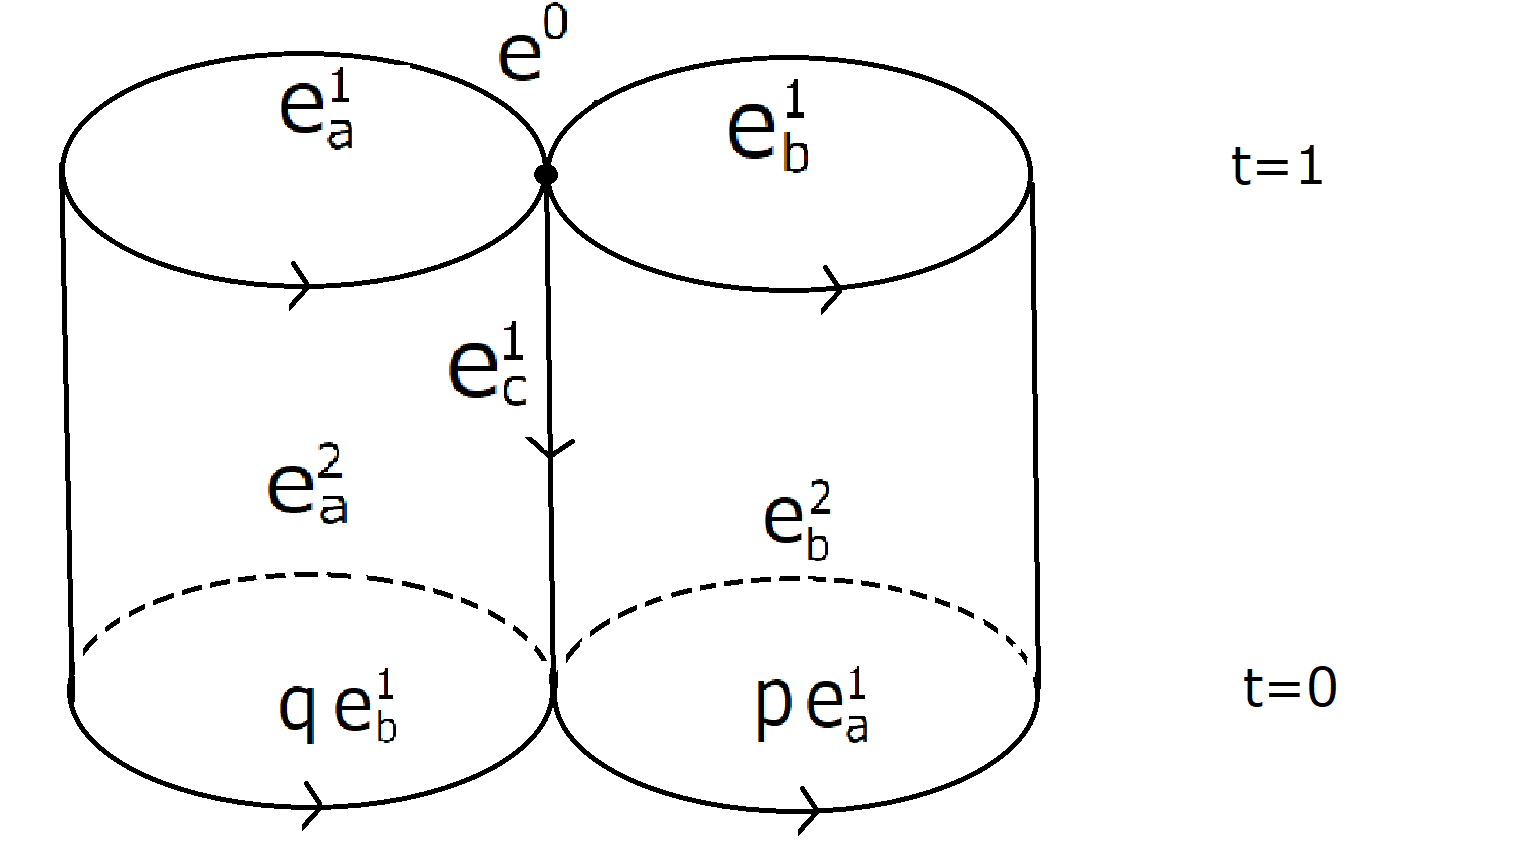
\includegraphics[width=5cm]{H31expert05_01.png}
\end{center}

この対になった円筒は、$X \tm I$および$Y$を表している。上下の円盤に見える部分は円周であり、ちくわを2つくっつけたような形をしている。側面も輪郭しか書かれていないが、面になっている。垂直方向が$I$成分を表しており、上が$t=1$で下が$t=0$であるものとしよう。また右を実軸のプラス方向、奥を虚軸のプラス方向とする。上部にある点は原点を表す。図に$e$と書かれているのはセルである。それぞれ具体的には次のように与えられる。
\begin{align*}
  e^0 &= (0,1) \\
  e^1_a &= \setmid{ (-1+e^{i\grt},1) }{0 < \grt < 2\pi } \\
  e^1_b &= \setmid{ (1-e^{i\grt},1) }{0 < \grt < 2\pi } \\
  e^1_c &= \setmid{ (0,t) }{0 < t < 1 } \\
  e^2_a &= \setmid{ (-1+e^{i\grt},t) }{0 < \grt < 2\pi , 0 < t < 1 } \\
  e^2_b &= \setmid{ (1-e^{i\grt},t) }{0 < \grt < 2\pi , 0 < t < 1 }
\end{align*}
このとき、次に注意する。
\begin{align*}
  e^0 &= (0,0) \\
  pe_a^1 &= \setmid{ (1-e^{i\grt},0) }{0 < \grt < 2\pi } \\
  qe_b^1 &= \setmid{ (-1+e^{i\grt},1) }{0 < \grt < 2\pi }
\end{align*}
さて以上の準備の下セル複体のホモロジーを計算しよう。$Y$の$0$セル、$1$セル、$2$セルの数はそれぞれ$1,3,2$個なので
\[
\xymatrix{
0 \ar[r] & \Z^2 \ar[r]^{\del} & \Z^3 \ar[r]^{\grs} & \Z \ar[r] & 0
}
\]
という図式に表されるような状況になっている。まず$\grs$だが、$0$セルはただひとつしかないのでこれはゼロ写像である。よって$H_0(Y)=\Z$がわかる。
次に$\del$を計算する。次の図

\begin{center}
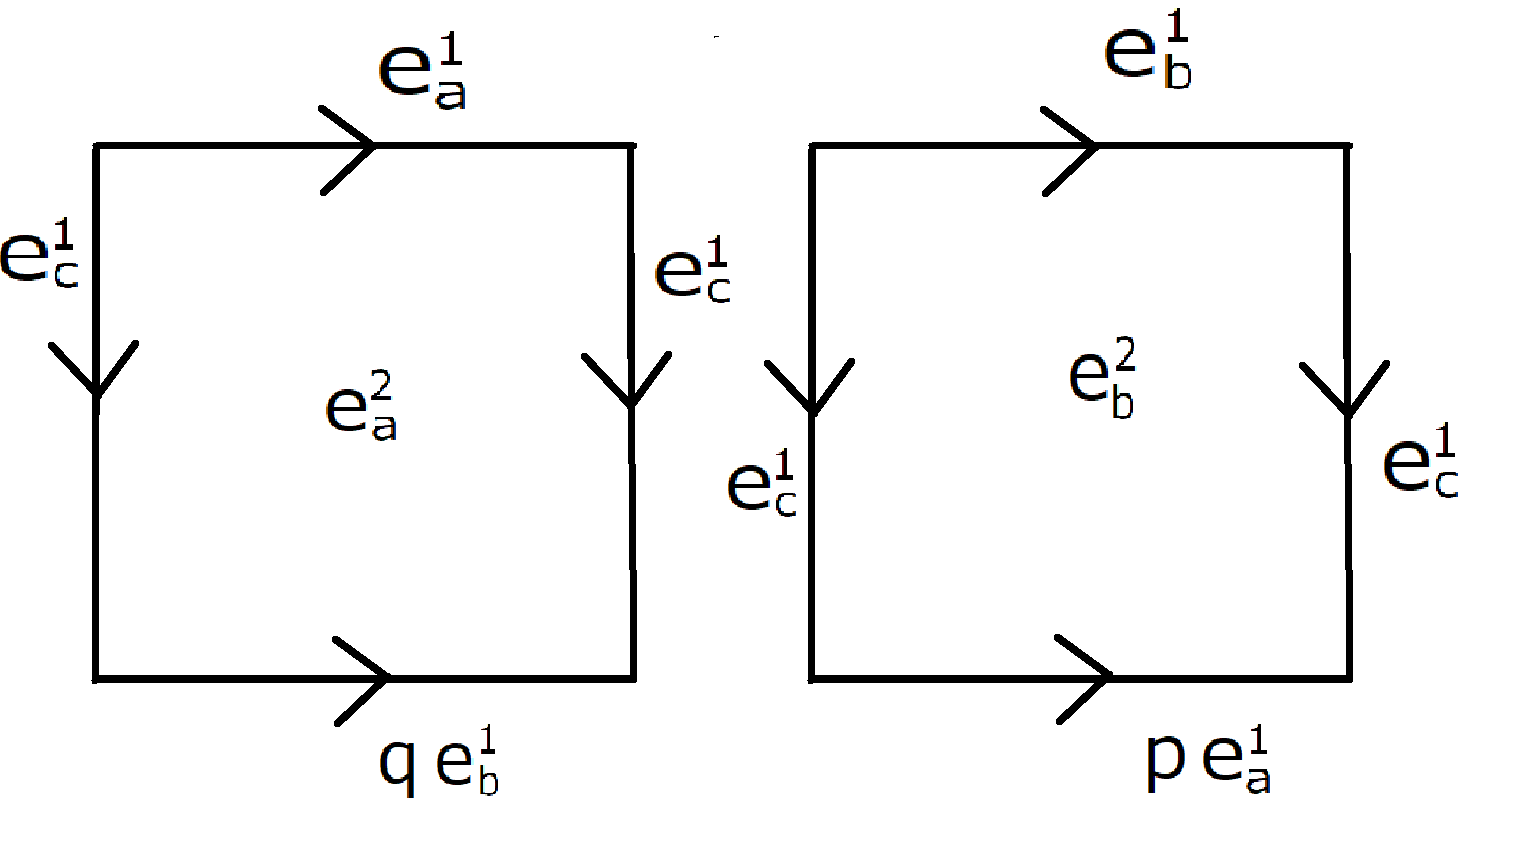
\includegraphics[width=5cm]{H31expert05_02.png}
\end{center}

のような状況になっているので
\[
\del(e_a^2) = e_a^1 - qe_b^1 \quad \del(e_b^2) = e_b^1 - pe_a^1
\]
である。したがって$\del$は次の行列
\[
\del = \pmat{
1 & -p \\
-q & 1 \\
0 & 0
}
\]
で表される写像である。この行列の階数は$pq =1$のとき$1$でそうでないとき$2$である。よって$pq = 1$のとき
\begin{align*}
  H_1(Y) &= \Z^3 / \Im \del \\
  &= \Z^2 \\
  H_2(Y) &= \Ker \del \\
  &= \Z
\end{align*}
である。$pq \neq 1$ならば
\begin{align*}
  H_1(Y) &= \Z^3 / \Im \del \\
  &= (a \Z \oplus  b \Z \oplus c \Z)  / (a - qb, b - pa) \\
  &= (a \Z \oplus  b \Z )  / ( (1-pq)a, b - pa) \oplus c \Z \\
  &= \Z / (1-pq)\Z \oplus \Z \\
  H_2(Y) &= \ker \del \\
  &= 0
\end{align*}
である。以上により求めるホモロジーは、$pq = 1$のとき
\[
H_i(Y) = \begin{cases}
\Z &(i=0,2) \\
\Z^2 &(i=1) \\
0 &(\text{otherwise})
\end{cases}
\]
であり、$pq \neq 1$のとき
\[
H_i(Y) = \begin{cases}
\Z &(i=0) \\
\Z / (pq-1)\Z \oplus \Z &(i=1) \\
0 &(\text{otherwise})
\end{cases}
\]
\end{sol}


\newpage

\section{平成30年度 基礎科目}

\subsubsection{} %{問1}
\lbar{
広義積分
\[
\iiint_V \f{1}{(1+x^2 + y^2)z^{ \f{3}{2} }} \; dx dy dz
\]
を計算せよ。ただし、$V=\setmid{(x,y,z) \in \R^3}{x^2+y^2 \leq z}$とする。
}

\begin{sol}
  極座標変換$(x,y,z) \mapsto (r,\grt, z)$を考える。このとき$dx dy dz = r dr d\grt dz$であり、
  \begin{align*}
    \iiint_V \f{1}{(1+x^2 + y^2)z^{ \f{3}{2} }} \; dx dy dz &= \int_{0}^{2\pi} \; d\grt \int_{0}^{\infty} \f{r}{1+r^2} \left( \int_{r^2}^{\infty} z^{ -\f{3}{2}  } \; dz \right) \; dr \\
    &= 2\pi \int_{0}^{\infty} \f{r}{1+r^2} \left[ (-2)z^{-\f{1}{2}} \right]^{\infty}_{r^2} \; dr \\
    &= 4\pi \int_{0}^{\infty} \f{r}{1+r^2} \f{1}{r} \; dr \\
    &= 4\pi \int_{0}^{\infty} \f{1}{1+r^2} \; dr \\
    &= 4\pi \cdot \f{\pi}{2} \\
    &= 2\pi^2
  \end{align*}
  と計算できる。
\end{sol}

\newpage

\subsubsection{} %{問2}
\lbar{
$a,b$を実数とする。実行列
\[
A = \begin{pmatrix}
1 & 1 & a & b \\
0 & 1 & 2 & 0 \\
2 & 0 & 1 & 4
\end{pmatrix}
\]
について、以下の問に答えよ。
\begin{description}
\item[(1)] 行列$A$の階数を求めよ。
\item[(2)] 連立1次方程式
\[
A \begin{pmatrix}
x_1 \\
x_2 \\
x_3 \\
x_4
\end{pmatrix} = \begin{pmatrix}
1 \\ 1 \\ 1
\end{pmatrix}
\]
が解を持つような実数$a,b$をすべて求めよ。
\end{description}
}

\begin{sol} ${}$
  \begin{description}
    \item[(1)] ある行に別の行の定数倍を足す操作を繰り返すと
    \begin{align*}
      A &\sim \begin{pmatrix}
      1 & 1 & a & b \\
      0 & 1 & 2 & 0 \\
      0 & -2 & 1-2a & 4-2b
      \end{pmatrix} \\
      &\sim \begin{pmatrix}
      1 & 1 & a & b \\
      0 & 1 & 2 & 0 \\
      0 & 0 & 5-2a & 4-2b
      \end{pmatrix}
    \end{align*}
    と変形できる。したがって$\rank A \geq 2$であり、$(a,b) = (\f{5}{2}, 2)$のときは$\rank A =2$で、$(a,b) \neq  (\f{5}{2}, 2)$のときは$\rank A =3$である。
    \item[(2)] $(a,b) \neq  (\f{5}{2}, 2)$ならば、$A \colon \R^4 \to \R^3$は全射なので、解がある。$(a,b) = (\f{5}{2}, 2)$のとき、拡大係数行列を考えると
    \begin{align*}
      \begin{pmatrix}
      1 & 1 & \f{5}{2} & 2 & 1 \\
      0 & 1 & 2 & 0  & 1 \\
      2 & 0 & 1 & 4 & 1
      \end{pmatrix} \sim
      \begin{pmatrix}
      1 & 1 & \f{5}{2} & 2 & 1 \\
      0 & 1 & 2 & 0  & 1 \\
      0 & -2 & -4 & 0 & -1
      \end{pmatrix}
      \sim \begin{pmatrix}
      1 & 1 & \f{5}{2} & 2 & 1 \\
      0 & 1 & 2 & 0  & 1 \\
      0 & 0 & 0 & 0 &  1
      \end{pmatrix}
    \end{align*}
    となるので、解はない。
  \end{description}
\end{sol}


\newpage

\subsubsection{} %{問 3}
\barquo{
広義積分
\[
\int_{-\infty}^{\infty} \f{\cos(\pi x)}{1 + x^2 + x^4} \; dx
\]
を求めよ。
}
\begin{sol}
$f$, $F$を
    \[
    f(x) = \f{\cos(\pi x)}{1 + x^2 + x^4}, \quad F(z) = \f{e^{\I \pi z}}{1 + z^2 + z^4}
    \]
により定める。$x \in \R$なら$f(x) = \Re F(x)$である。

ここで分母の$1 + z^2 + z^4$を因数分解しておく。
$\zeta = \exp(\I \pi / 3) = (1 + \sqrt{-3})/ 2$とする。$1+z + z^2$の根は$1$の原始$3$乗根であることから
\begin{align*}
  z^4 + z^2 + 1 &= (z^2 - \zeta^2)(z^2 - \zeta^4) \\
  &= (z - \zeta )(z + \zeta) (z - \zeta^2)(z + \zeta^2)
\end{align*}
である。

上反平面に含まれる半径$R$の半円を$C_R$とする。留数定理により、任意の$R > 1$について
\[
2 \pi \I ( \Res_{z=\zeta} F + \Res_{z=\zeta^2} F ) = \int_{-R}^R F(x) \; dx + \int_{C_R} f(z) \; dz
\]
が成り立つ。

ここで、
\begin{align*}
  \abs{\int_{C_R} f(z) \; dz } &\leq \int_0^{\pi} \abs{ \f{R \exp(\I R \pi e^{\I \grt}) }{ 1 + R^2e^{2 \I \grt} +  R^4e^{4 \I \grt}} } \; d\grt \\
  &\leq  \int_0^{\pi} \f{R e^{- R \pi \sin \grt} }{R^4 - R^2 - 1}   \; d\grt \\
  &\leq \f{R  }{R^4 - R^2 - 1}  \int_0^{\pi} \; d\grt \\
  &\leq  \f{R \pi }{R^4 - R^2 - 1}
\end{align*}
だから、$R \to \infty$のとき$\int_{C_R} f(z) \; dz \to 0$である。したがって
\[
 \int_{-\infty}^{\infty} f(x) \; dx =  \Re( 2 \pi \I ( \Res_{z=\zeta} F + \Res_{z=\zeta^2} F ) )
\]
であることがわかる。

実際に留数を計算しよう。詳細は省略するが、堅実な計算により
\begin{align*}
  \Res_{z=\zeta} F &= \f{ \exp(\I \pi \f{1 + \sqrt{-3}}{2} ) }{(2\zeta) (\zeta - \zeta^2) (\zeta + \zeta^2)  } \\
  &= \f{ - \I \exp(- \f{\sqrt{3}\pi}{2} ) }{2(1 - \zeta^2)} \\
  \Res_{z=\zeta^2} F &= \f{ \exp(\I \pi \f{-1 + \sqrt{-3}}{2} ) }{(\zeta^2 - \zeta) (\zeta^2 + \zeta) (\zeta^2 + \zeta^2)  } \\
  &=  \f{ - \I \exp(- \f{\sqrt{3}\pi}{2} ) }{2(1 + \zeta)}
\end{align*}
がわかる。$\gra = \exp(- \f{\sqrt{3}\pi}{2} )$とおこう。すると
\begin{align*}
  2 \pi \I ( \Res_{z=\zeta} F + \Res_{z=\zeta^2} F ) &= \gra \pi \left( \f{1}{1 - \zeta^2} + \f{1}{1+ \zeta} \right) \\
  &= \gra \pi \left( \f{2 - \zeta}{ 1 - \zeta^2} \right) \\
  &= \gra \pi
\end{align*}
である。$\gra \in \R$だから、
\[
 \int_{-\infty}^{\infty} f(x) \; dx = e^{- \f{\sqrt{3}\pi}{2} } \pi
\]
が結論される。
\end{sol}
\newpage

\subsubsection{} %{問 4}
\lbar{
閉区間$[0,1]$上の実数値関数列$\{ f_n \}^{\infty}_{n=1}$について、各$f_n$は広義単調増加であるものとする。つまり、$0 \leq x < y \leq 1$なら、$f_n(x) \leq f_n(y)$である。この関数列$\{ f_n \}^{\infty}_{n=1} $が$n \to \infty$で関数$f$に各点収束したとする。
\begin{description}
  \item[(1)] 任意の$0 \leq x < y \leq 1$に対し、不等式
  \[
  \sup_{x \in [x,y]} \abs{f_n(z) - f(z)} \leq \max\{ \abs{f_n(x)- f(y)}, \abs{f_n(y)-f(x)}  \}
  \]
  を示せ。
  \item[(2)] 関数$f$が連続であるとき、関数列$\{ f_n \}^{\infty}_{n=1}$は$f$に$[0,1]$上で一様収束することを示せ。
\end{description}
}
\begin{sol} ${}$
\begin{description}
  \item[(1)] まず$f$が広義単調増加であることを示す。$0 \leq x < y \leq 1$とする。$\ve > 0$が与えられたとする。$f_n$が$f$に各点収束することにより
  \begin{align*}
    n \geq N(x) \to \abs{f(x) - f_n(x)} < \ve \\
      n \geq N(y) \to \abs{f(y) - f_n(y)} < \ve
  \end{align*}
  なる$N(x), N(y)$の存在がわかる。したがって$n \geq \max\{ N(x), N(y) \}$のとき
  \begin{align*}
    f(y) - f(x) + 2\ve &= (f(y) + \ve ) - f(x) + \ve \\
    &\geq f_n(y) - f(x) + \ve &(-\ve < f(y)-f_n(y) < \ve \text{より}) \\
    &\geq f_n(y) - f_n(x) &(-\ve < f(x)-f_n(x) < \ve \text{より}) \\
    &\geq 0
  \end{align*}
  がわかる。$\ve > 0$は任意だったから、$f(y) \geq f(x)$がわかる。つまり$f$は広義単調増加である。

  したがって任意の$z \in [x,y]$に対して
\begin{align*}
f_n(z) - f(z) \leq f_n(y) - f(x) \\
f(z) - f_n(z) \leq f(y) - f_n(x)
\end{align*}
が成り立つので、
\[
\abs{f_n(z) - f(z)} \leq \max\{ \abs{f_n(x)- f(y)}, \abs{f_n(y)-f(x)}  \}
\]
である。右辺は$z$の取り方によらないので、
\[
\sup_{x \in [x,y]} \abs{f_n(z) - f(z)} \leq \max\{ \abs{f_n(x)- f(y)}, \abs{f_n(y)-f(x)}  \}
\]
がいえた。
\item[(2)] $\ve > 0$が与えられたとする。$I = [0,1]$はコンパクトなので、$f$は一様連続であることまでいえる。そこで
\[
\abs{x -y} < \grd \to \abs{f(x) - f(y)} < \ve
\]
なる$\grd > 0$がある。この$\grd$を固定し、$B(z) = [z - \grd/3, z + \grd/3] \cap I$とする。$\grd > 0$なので、$I = \bigcup_{i=1}^m B(z_i)$なる有限個の$z_i \in I$をとることができる。$B(z_i ) = [x_i, y_i]$と表すことにする。

$f_n$は$f$に各点収束しているので、
\begin{align*}
  n \geq N(x_i) &\to \abs{f(x_i) - f_n(x_i)} < \ve \\
  n \geq N(y_i) &\to \abs{f(y_i) - f_n(y_i)} < \ve
\end{align*}
なる$N(x_i), N(y_i)$がある。そこで
\[
n \geq \max\{ N(x_1), \cdots , N(x_m) , N(y_1) , \cdots , N(y_m)  \}
\]
とする。このとき
\begin{align*}
  \abs{f_n(x_i)- f(y_i) } &\leq \abs{ f_n(x_i) - f(x_i) } + \abs{ f(x_i) - f(y_i) } \\
  &\leq 2\ve \\
\abs{f_n(y_i)- f(x_i) }  &\leq \abs{ f_n(y_i) - f(y_i) } + \abs{ f(y_i) - f(x_i) } \\
&\leq 2\ve
\end{align*}
が成り立つ。したがって(1)により、不等式評価を端点に押しつけることができて
\begin{align*}
\sup_{z \in I } \abs{f_n(z) - f(z)} &\leq \max_{1 \leq i \leq m} \sup_{x \in [x_i,y_i]} \abs{f_n(z) - f(z)} \\
&\leq \max_{1 \leq i \leq m} \max\{ \abs{f_n(x_i)- f(y_i)}, \abs{f_n(y_i)-f(x_i)}  \} \\
&\leq 2\ve
\end{align*}
である。これで一様収束がいえた。
\end{description}
\end{sol}

\newpage

\subsubsection{} %{問 5}
\barquo{
$p$を素数とし、$\F_p = \Z / p \Z$を位数$p$の有限体とする。行列の乗法による群$G$を
\[
G = \setmid{ \pmat{1 & a & b \\ 0 & 1 & c \\ 0 & 0 & 1 } }{a,b,c \in \F_p}
\]
で定める。このとき、$G$から乗法群$\C^{\tm} = \C \sm \{ 0 \}$への準同形写像の個数を求めよ。
}
\begin{sol}
 次の事実に注意する。
\lem{
$\pi \colon G \to G/[G,G]$は自然な写像とする。すると$\pi$が誘導するAbel群の準同型
\[
p \colon \Hom(G/[G,G], \C^{\tm}) \to \Hom(G, \C^{\tm})
\]
は同型である。
}
\begin{proof}
$\pi$は全射なので、$p$は単射である。また$p$は全射でもある。なぜならば!$g \in \Hom(G, \C^{\tm})$が任意に与えられたとしよう。このとき$\C^{\tm}$がAbel群であることにより、$[G,G] \subset \Ker g$が成り立つ。したがって準同型定理により、$p(f) = g$となるような$f \in \Hom(G/[G,G], \C^{\tm})$が存在する。ゆえにかくのごとし。これで$p$が同型であることがいえた。
\end{proof}

 したがって$G/[G,G]$の構造を決定すればよい。そのためにまず$[G,G]$を決定する。
    \[
    A = \pmat{1 & a & b \\ 0 & 1 & c \\ 0 & 0 & 1},  \quad B = \pmat{1 & \grd & \beta \\ 0 & 1 & \grg \\ 0 & 0 & 1}
    \]
    とおく。($\gra$は$a$と間違えやすいので、$\grd$を使った。)計算すれば、このとき
    \begin{align*}
    ABA^{-1}B^{-1} = \pmat{1 & 0  & a \grg - c \grd \\ 0 & 1 & 0 \\ 0 & 0 & 1 }
  \end{align*}
  であることが判る。$a \grg - c \grd$は$\F_p$全体をわたるので、
  \[
  [G,G] = \setmid{ \pmat{1 & 0 & d \\ 0 & 1 & 0 \\ 0 & 0 & 1} }{d \in \F_p }
  \]
  が結論できる。

  次に$G/[G,G]$の構造を決定したい。
  \[
  E_1 = \pmat{1 & 1 & 0 \\ 0 & 1 & 0 \\ 0 & 0 & 1}, \quad E_2 =  \pmat{1 & 0 & 0 \\ 0 & 1 & 1 \\ 0 & 0 & 1}
  \]
  とし、$E_1, E_2 \in G/ [G,G]$と見なす。
  \[
  E_1^n = \pmat{1 & n & 0 \\ 0 & 1 & 0 \\ 0 & 0 & 1}, \quad E_2^m =  \pmat{1 & 0 & 0 \\ 0 & 1 & m \\ 0 & 0 & 1}
  \]
  なので、$E_1, E_2$は位数がちょうど$p$である。また、$C = E_1^n = E_2^m$とするとき
  \[
  1 = E_1^n E_2^{-m} = \pmat{ 1 & n & -nm \\ 0 & 1 & -m \\ 0 & 0 & 1}
  \]
  だから$n=m=0$が従う。つまり$\kakko{E_1} \cap \kakko{E_2} = 1$である。$G/[G,G]$はAbel群なので積による準同形
  $
\kakko{E_1} \tm \kakko{E_2} \to G/[G,G]
  $
  がある。これは、$\kakko{E_1} \cap \kakko{E_2} = 1$により単射である。位数$p^2$の有限群の間の単射なので、とくに同型である。よって$G/[G,G] \cong \F_p^2$がわかった。

あとは$\# \Hom(\F_p^2, \C^{\tm})$を求めよう。これは$\# \Hom(\F_p,\C^{\tm})$の$2$乗である。$\# \Hom(\F_p,\C^{\tm}) = p$より求める答えは$p^2$である。

\end{sol}

\newpage

\subsubsection{} %{問6}
\barquo{
$\R^4$の部分空間$M$を
\[
M = \setmid{(x,y,z,w) \in \R^4}{x^2 + y^2 + z^2 + w^2 = 1, \; xy + zw = 0}
\]
で定める。
\begin{description}
  \item[(1)] $M$が$2$次元微分可能多様体になることを示せ。
  \item[(2)] $M$上の関数$f$を
  \[
  f(x,y,z,w) = x
  \]
  で定めるとき、$f$の臨界点をすべて求めよ。ただし、$p \in M$が$f$の臨界点であるとは、$p$における$M$の局所座標$(u,v)$に関して
  \[
  \f{\del f}{\del u}(p) =   \f{\del f}{\del v}(p) = 0
  \]
  となることである。
\end{description}
}
\begin{sol} ${}$
  \begin{description}
    \item[(1)] $F \colon \R^4 \to \R^2$を
      \[
      F(x,y,z,w) = \pmat{x^2 + y^2 + z^2 + w^2 - 1 \\ xy+zw}
      \]
      により定める。$M = F^{-1}(O)$である。$p=(x,y,z,w) \in M$としよう。$p$におけるヤコビアンを計算すると
      \[
      JF_p = \pmat{2x & 2y & 2z & 2w \\ y & x & w & z }
      \]
      である。ここで$p \neq O$より$\rank JF_p \geq 1$である。仮に$\rank JF_p = 1$ならば、$JF_p$の2つの行は1次従属である。よって、$p \neq O$により$(y , x, w,z) = c(x,y,z,w)$なる定数$c \in \R$がある。このとき$xy + zw = c(x^2 + z^2) = 0$となり、$p \neq O$に矛盾。よって$\rank JF_p = 2$である。ゆえに$p$は$F$の正則点であり、$M$は$\R^4$の$2$次元部分多様体。
      $F$は$\bfC^{\infty}$級なので、$M$は微分可能になる。
      \item[(2)] $f \colon M \to \R$の$\R^4$への自然な拡張を$\wt{f}$とする。このとき$p \in M$に対して$T_p M \subset \R^4$と見なせば、$T_p M = \Ker JF_p$であるから、
      \begin{align*}
        \text{$p$が$f$の臨界点} &\iff \rank (df_p \colon T_p M \to \R) < 1 \\
        &\iff \dim \Ker df_p = 2 \\
        &\iff \dim \Ker \pmat{JF_p \\ J\wt{f}_p} = 2 \\
        &\iff \rank \pmat{2x & 2y & 2z & 2w \\ y & x & w & z \\ 1  & 0 & 0 & 0} = 2 \\
        &\iff \rank \pmat{0 & 2y & 2z & 2w \\ 0 & x & w & z \\ 1  & 0 & 0 & 0} = 2
      \end{align*}
      である。いま$p=(x,y,z,w) \in M$が臨界点であったと仮定する。このとき$(x,w,z)$と$(y,z,w)$は1次従属である。よって$(y,w,z) = 0$かまたは、ある$c \in \R$が存在して$(x,w,z)=  c(y,z,w )  $である。$(y,w,z) = 0$なら$p =(\pm 1, 0, 0 ,0)$である。$(x,w,z)=  c(y,z,w )  $なら、$c(y^2 + z^2)=0$より$p=(0, \pm 1, 0, 0)$である。

      逆に$p=(\pm 1, 0, 0 ,0), (0, \pm 1, 0, 0)$ならば$p \in M$であり、$f$の臨界点であることはあきらかなので、臨界点はこれですべて求まったことになる。
  \end{description}

\end{sol}


\newpage

\subsubsection{} %{問7}
\barquo{
$A$を実正方行列、$k$を正の整数とし、$\rk (A^{k+1}) = \rk (A^k)$が成り立つとする。このとき、任意の整数$m \geq k$に対し、$\rk (A^m) = \rk (A^k)$であることを証明せよ。ここで行列$X$に対し、$\rk(X)$は$X$の階数を表す。
}
\begin{proof}
  仮定から、$\Ker A^{k+1}$の次元と$\Ker A^k$の次元は等しい。包含関係があって次元が等しいので、$\Ker A^{k+1} = \Ker A^k$である。ここで$m \geq k +2$に対して$x \in \Ker A^m$と仮定する。そうすると$A^m x = A^{m-k-1} A^{k+1} x$だから$A^{m-k-1} x \in \Ker A^{k+1} = \Ker A^k$である。よって$A^k A^{m-k-1} x = A^{m-1} x = 0$であり、$x \in \Ker A^{m-1}$がわかる。これを帰納的に繰り返して、
  $\Ker A^m \subset \Ker A^{m-1} \subset \cdots \subset \Ker A^k$を得る。逆はあきらかなので$\Ker A^m = \Ker A^k$である。よってとくに階数も等しい。
\end{proof}


\newpage

\bfsection{平成30年度 専門科目}

\bfsubsection{問1}
\barquo{
$k$を可換体とする。$k[X,Y]$を$k$上の2変数多項式環として、$f \in k[X,Y]$の零点集合$V(f)$を
\[
V(f) = \setmid{(a,b) \in k \tm k}{f(a,b) = 0}
\]
によって定義する。次の2条件は同値であることを示せ。
\begin{description}
  \item[(1)] $k$は代数的閉体ではない。
  \item[(2)] $V(f) = \{(0,0)\}$となる$f \in k[X,Y]$が存在する。
\end{description}
}
\begin{sol}${}$
\begin{description}
  \item[(1)$\To$(2)] $k$は代数的閉体ではないので、ある1次以上の多項式$g \in k[X]$であって、$k$上根を持たないものが存在する。$n = \rm{dim}\ g$とおいて、
  \[
  f(X,Y)= Y^n g \left(\frac{X}{Y} \right)
  \]
  とおく。別の言い方をすれば$g(X)= X^n + a_{n-1}X^{n-1} + \cdots + a_1X + a_0$とするとき, $f(X,Y)= X^n + a_{n-1}X^{n-1}Y + \cdots + a_1XY^{n-1} + a_0Y^n$である。$X \in k$, $Y \in k \sm \{0\}$に対して$Y^n$と$g(X/Y)$は決して0にならないので、$f(X,Y)=0$となるのは$Y=0$のときだけである。$f(X,0)=X^n$なので、
  $V(f) =\{ (0,0)\}$が成り立つ。
  \item[(2)$\To$(1)] 対偶をとり、$k$が代数閉体であってかつ$V(f) =\{ (0,0)\}$となる$f \in k[X,Y]$が存在すると仮定し矛盾を示そう。このとき$k$は無限体($k$が有限体であっても、アイゼンシュタイン多項式は無限個あるため)であることに注意する。またここではそもそも$k$は零環ではないとして考えていることにも注意する。

  さて$a,b \in k^{\tm}$を任意にとると、$f(a,Y) \in k[Y]$、$f(X,b) \in k[X]$は決して0にならないので、定数でなければならない。
  このとき$f(a,Y)=f(a,b)=f(X,b)$であるので、常にこの2つは一致する。割り算を実行して
  \begin{align*}
    f(X,Y) &= (X-a)g(X,Y) + f(a,Y) \\
    f(X,Y) & =(Y-b)h(X,Y)+f(X,b)
  \end{align*}
  なる$g, h \in k[X,Y]$をとってくる。すると辺々引いて
  \[
  0 = (X-a)g(X,Y) - (Y-b)h(X,Y)
  \]
  が成り立つ。この等式は任意の$a,b \in k^{\times}$について成り立つので、$g=h=0 \in k[X,Y]$が判る。ゆえに$f$は定数となるがこれは矛盾。
  \item[別解] (2)$\To$(1)を示す部分についてはHilbertの零点定理を知っていればすこし議論を省略できる。$k$が代数閉体だと仮定し$V(f) =\{ (0,0)\}$となる$f \in k[X,Y]$が存在するとしよう。$k[X,Y]$はUFDなので、$f$は既約であるとしてよい。すると$(f)$は根基イデアルなのでHilbertの零点定理により$(f) = (X,Y)$である。しかし右辺は単項イデアルではないので矛盾。
\end{description}
\end{sol}


\newpage





\bfsubsection{問2}
\barquo{
$p$を素数, $k,m$を正の整数で、$k$と$p^2 - p$は互いに素であるとする。位数$kp^m$の有限群$G$が次の性質を満たす部分群$N,H$をもつとする。
\begin{description}
  \item[(1)] $N$は位数$p^m$の巡回群で$G$の正規部分群である。
  \item[(2)] $H$は位数$k$の群である。
\end{description}
このとき、$G$は$N$と$H$の直積であることを示せ。
}
\begin{sol}
  $H \lhd G$を示せば十分である。(付録の「半直積とGaois群」を参照のこと) $N \lhd G$なので、$H$の共役による$N$への作用$\Phi \colon H \rightarrow \Aut N$を$\Phi_h(q)=hqh^{-1}$により定義できる。$H / \Ker \Phi$は$\Aut N$の部分群とみなせる。
  \begin{align*}
    \#(\Aut N) &= \#((\Z/ p^m \Z)^{\tm}) \\
    &= p^m - p^{m-1}
  \end{align*}
  なので、$\#(H / \Ker \Phi)$は$\# H= k$と$ p^m - p^{m-1}$の両方を割り切る。したがって$\#(H / \Ker \Phi) \leq \gcd (k,p^m - p^{m-1})$であるが、右辺は仮定により1だから$\Phi$は自明な作用であって、$H$の元はすべての$N$の元と可換である。

  よって、$G$の元$g=hq \; (h \in H, q \in N)$と$x \in H$に対して$g^{-1}xg = x^g =x^{hq} = (x^h)^q = x^h \; \in H$だから、$H \lhd G$が言えた。
\end{sol}

\newpage


\bfsubsection{問3}
\barquo{
多項式$X^7 - 11$の有利数体$\Q$上の最小分解体を$K \subset \C$とする。このとき、次の問に答えよ。
\begin{description}
  \item[(1)] 拡大次数$[K:\Q]$を求めよ。
  \item[(2)] $\Q$と$K$の間の($\Q$でも$K$でもない)真の中間体の個数を求めよ。
  \item[(3)] 上記(2)の中間体のうち、$\Q$上Galois拡大になるものの個数を求めよ。
\end{description}
}
\begin{sol} ${}$
\begin{description}
  \item[(1)] $\gro = \exp (2\pi \sqrt{-1}/7)$とする。あきらかに$K = \Q(\gro, \sqrt[7]{11})$である。状況を図式で表すと次のようになる。
  \[
  \xymatrix{& K &  \\  \Q(\gro) \ar[ur]^{\leq 7} & & \Q(\sqrt[7]{11}) \ar[ul]_{\leq 6} \\  &  \Q \ar[ul]^{6} \ar[ur]_{7} &
  }
  \]
  円分体の一般論から$6= [\Q(\gro):\Q]$である。また$X^7 - 11$はEisenstein多項式なので既約であり$7=[\Q(\sqrt[7]{11}):\Q]$である。$7$と$6$は互いに素なので$\Q(\gro) \cap \Q(\sqrt[7]{11}) = \Q$である。
  $\Q(\gro) / \Q$はGalois拡大なので、Galois拡大の推進定理により$\Gal(K/ \Q(\sqrt[7]{11})) \cong \Gal(\Q(\gro) / \Q)$であり、とくに$[K: \Q(\sqrt[7]{11})] = [\Q(\gro):\Q] = 6$である。したがって、$[K:\Q]=42$である。
  \item[(2)] $G = \Gal(K/ \Q)$とする。付録「半直積とGalois群」により、$G$は半直積
  \[
\Gal(K/ \Q(\gro)) \rtimes \Gal(K/ \Q(\sqrt[7]{11}))
  \]
  と同型である。素数次数なので$\Gal(K/ \Q(\gro)) = \Z / 7 \Z$であり、
  円分体の一般論から
\[
\Gal(K/ \Q(\sqrt[7]{11})) \cong \Gal(\Q(\gro) / \Q) = (\Z / 7 \Z)^{\tm} = \Z / 6 \Z
\]
  である。つまりともに有限巡回群である。$\grs \in \Gal(K/ \Q(\gro))$を$\grs(\sqrt[7]{11}) = \sqrt[7]{11} \gro$により定め、
  $\tau \in \Gal(K/ \Q(\sqrt[7]{11}))$を$\tau(\gro) = \gro^3$により定める。$\grs$, $\tau$はそれぞれ生成元となる。$\tau \grs \tau^{-1}(\sqrt[7]{11}) = \sqrt[7]{11} \gro^3$より
  $\tau \grs \tau^{-1} = \grs^3$である。したがって次の表示
  \[
  G \cong \setmid{\grs,\tau}{\grs^7 = \tau^6 = 1, \tau \grs \tau^{-1} = \grs^3} \cong \Z / 7 \Z \rtimes \Z / 6 \Z
  \]
  を得る。

  Galoisの基本定理により、$G$の自明でない部分群の個数を求めればよい。そこでまずすべての元の位数を決定する。$\kakko{\grs} \rtimes \kakko{\tau} \to \kakko{\tau}$は群準同型なので、$x = \grs^i \tau^j \in G$の共役は$\grs^{*} \tau^j$という形をしている。具体的には
    \begin{align*}
      \grs x \grs^{-1} &= \grs \grs^i \tau^j \grs^{-1} \\
      &= \grs \grs^i (\tau^j \grs^{-1} \tau^{-j} ) \tau^j \\
      &= \grs \grs^i (\grs^{3^j})^{-1} \tau^j \\
      &= \grs^{1 - 3^j} \grs^i \tau^j \\
      &= \grs^{1 - 3^j} x
    \end{align*}
    である。
  そこで共役元を求めることにより次のような位数の表をつくることができる。
  \begin{center}
  \begin{tabular}{ccc}
   \hline
位数 & 元 & 個数 \\
   \hline \hline
   1 & 1 & 1 \\
   2 & $\grs^i \tau^3 \; (0 \leq i \leq 6)$ &  7 \\
  3 & $\grs^i \tau^2 \; (0 \leq i \leq 6)$, $\grs^i \tau^4 \; (0 \leq i \leq 6)$ &  14  \\
  6 & $\grs^i \tau \; (0 \leq i \leq 6)$, $\grs^i \tau^5 \; (0 \leq i \leq 6)$ & 14 \\
  7 & $\grs^i \; ( 1 \leq i \leq 6)$ & 6
   \end{tabular}
  \end{center}
  次に部分群を列挙する作業に移る。$G$の位数は42なので、自明でない部分群の位数としてありえるのは$2,3,6,7,14,21$である。まず位数2の部分群は位数2の元と同じ数だけあるので、7個である。位数3の部分群は、素数位数なのですべて巡回群であり、生成元はひとつの群に対して2つある。よって位数3の部分群は$14/2 = 7$個ある。

  位数6の部分群$M \subset G$が与えられたとする。このとき次のような各行が完全な可換図式がある。
\[
\xymatrix{
1 \ar[r] & \Z / 7 \Z \ar[r]^-j &  \Z / 7 \Z \rtimes \Z / 6 \Z \ar[r]^-p & \Z / 6 \Z \ar[r] & 1 \\
1 \ar[r] & j^{-1}(M) \ar[r]^-j  \ar[u] & M  \ar[u] \ar[r]^-p & p(M) \ar[r] \ar[u] & 1
}
\]
$j^{-1}(M) = 1$でなくてはならないため、$M \cong p(M)$でありしたがって$M$は巡回群である。位数6の巡回群の生成元はひとつの群に対して2つなので、位数6の部分群は$14/2 = 7$個ある。
  位数7の部分群は、Sylow-7部分群なのですべて共役である。ところが$\kakko{\grs}$は正規部分群だったので、ひとつしかない。
  位数14の部分群は、Sylowの定理より位数2の元と位数7の元で生成される。したがって$\kakko{\grs, \tau^3}$しかない。よって1個。位数21の部分群も、Sylowの定理により位数3の元と位数7の元で生成される。したがって$\kakko{\grs, \tau^2}$しかない。よって1個。以上により、次の表のようになる。
  \begin{center}
  \begin{tabular}{ccc}
   \hline
位数 & 部分群 & 個数 \\
   \hline \hline
   2 & $\kakko{\grs^i \tau^3}  \; (0 \leq i \leq 6)$ &  7 \\
  3 & $\kakko{\grs^i \tau^2} \; (0 \leq i \leq 6)$ &  7  \\
  6 & $\kakko{\grs^i \tau} \; (0 \leq i \leq 6)$ & 7 \\
  7 & $\kakko{\grs}$ & 1 \\
  14 & $\kakko{\grs, \tau^3}$ & 1 \\
  21 & $\kakko{\grs, \tau^2}$ & 1
   \end{tabular}
  \end{center}
  したがって非自明な部分群は$7 + 7 + 7 + 1 + 1 + 1 = 24$個ある。
  \item[(3)] Galoisの基本定理により、$G$の自明でない正規部分群の個数を求めればよい。$x = \grs^i \tau^j \in G$の共役$\grs x \grs^{-1}$は$\grs^{1 - 3^j} x$
    であることを思い出そう。これをみると、位数$2,3,6$の群のなかに正規部分群は存在しない。また、位数7,14,21の群はすべて正規部分群である。よって自明でない正規部分群は3個である。
\end{description}
\end{sol}


\newpage

\section{平成29年度 基礎科目}

\subsubsection{} %{問1}
\barquo{
次の重積分を求めよ。
\[
\iint_D e^{- \max \{ x^2,y^2 \} } \ dx dy
\]
ここで$D=\setmid{(x,y) \in \R^2}{0 \leq x \leq 1, 0 \leq y \leq 1}$とする。
}
\begin{sol}
  $E = \setmid{(x,y) \in D}{x \geq y}$とおく。このとき
  \begin{align*}
    \iint_D e^{- \max \{ x^2,y^2 \} } \ dx dy &= 2 \iint_E e^{- x^2 } \ dx dy \\
    &= 2 \int_0^1 \left(  \int_0^x e^{-x^2} \ dy   \right) \ dx \\
    &= 2 \int_0^1 x e^{-x^2} \ dx \\
    &= \int_0^1 e^{-z} \ dz &(z = x^2 \text{とおいた}) \\
    &= 1 - e^{-1}
  \end{align*}
\end{sol}


\newpage


\subsubsection{} %{問2}
\barquo{
実行列
\[
A= \pmat{
1 & -2 & -1 & 1 & 0 \\
-2 & 5 & 3 & -2 & 1 \\
1& 1& 2 &0 &-1 \\
5&  0&  5&  3&  2 \\
}
\]
について、以下の問に答えよ。
\begin{description}
  \item[(i)] 連立一次方程式
  \[
  A \pmat{
  x_1 \\
  x_2 \\
  x_3 \\
  x_4 \\
  x_5
  }
  = \pmat{ 0\\ 0\\ 0\\ 0 }
  \]
  の解をすべて求めよ。
  \item[(ii)]
  連立一次方程式
  \[
  A \pmat{
  x_1 \\
  x_2 \\
  x_3 \\
  x_4 \\
  x_5
  }
  = \pmat{0 \\ -1 \\ 1\\  c}
  \]
  が解を持つような実数$c$をすべて求めよ。
\end{description}
}
\begin{sol} ${}$
  \begin{description}
    \item[(i)] 行列$A$に行基本変形を繰り返し行っていく。
    \begin{align*}
      A &= \pmat{
      1 & -2 & -1 & 1 & 0 \\
      -2 & 5 & 3 & -2 & 1 \\
      1& 1& 2 &0 &-1 \\
      5&  0&  5&  3&  2 \\
      } \\
      &\sim \pmat{
      1 & -2 & -1 & 1 & 0 \\
      0 & 1 & 1 & 0 & 1 \\
      0& 3& 3 &-1 &-1 \\
      0&  10&  10&  -2&  2 \\
      } & \pmat{ R_1 \\ R_2+2R_1 \\ R_3-R_1 \\ R_4-5R_1} \\
     &\sim \pmat{
      1 & 0 & 1 & 1 & 2 \\
      0 & 1 & 1 & 0 & 1 \\
      0& 0& 0 &-1 &-4 \\
      0&  0&  0&  -2&  -8 \\
      } & \pmat{ R_1+2R_2 \\ R_2 \\ R_3-3R_2  \\ R_4 -10R_2} \\
      &\sim \pmat{
        1 & 0 & 1 & 0 & -2 \\
        0 & 1 & 1 & 0 & 1 \\
        0& 0& 0 &1 &4 \\
        0&  0&  0&  0&  0 \\
        } & \pmat{R_1+R_3 \\ R_2 \\ -R_3 \\ R_4-2R_3 }
    \end{align*}
    したがって、$A\bfx=\bfzero$の解空間は$x_3,x_5 \in \R$で貼られる$2$次元実ベクトル空間
    \[
    S = x_3 \pmat{-1 \\-1 \\1 \\0 \\0 } + x_5 \pmat{2\\ -1\\ 0\\ -4\\ 1}
    \]
    である。
    \item[(ii)] 次の事実に気を付ける。
    \prop{
    $k$は体、$A$は$k$係数の$(n,m)$行列であり$\bfx \in k^m, \bfb \in k^n$であるとする。このとき$\bfx$についての一次方程式$A\bfx = \bfb$が解を持つことと、$\rank A = \rank (A \; \bfb)$は同値。
    }
    \begin{proof}
      まず次は同値である。
      \[
        \exists \bfx \; A\bfx = \bfb \iff \exists \bfx \;  \pmat{A & \bfb} \pmat{\bfx \\ -1} = \bfzero
      \]
      ここで、$\Ker A \to \Ker (A \; \bfb) \st \bfx \mapsto {}^t(\bfx \; 0)$によって$\Ker A$は$\Ker (A \; \bfb)$の部分空間$\Ker (A \; \bfb) \cap \setmid{\bfy \in k^{m+1}}{y_{m+1}=0}$だと思えることに気を付けると
      \begin{align*}
      \exists \bfx \; A\bfx = \bfb &\iff \dim \Ker (A \; \bfb) > \dim  \Ker A \\
        &\iff 0 \leq \rank (A \; \bfb) - \rank A < 1 \\
        &\iff \rank A = \rank (A \; \bfb)
      \end{align*}
      であることがわかる。
    \end{proof}
    (ii)の解答に戻る。$\bfb = {}^t(0 \ -1 \;  1 \; c)$とおく。拡大係数行列$(A \; \bfb)$は行基本変形により
    \[
    (A \; \bfb) \sim \pmat{1& 0& 1&  0& -2& 2 \\ 0 &1& 1& 0& 1& -1 \\ 0& 0& 0& 1& 4& -4 \\ 0& 0& 0& 0& 0& c+2}
    \]
    と変形できる。したがって求める$c$の値は$c=-2$である。
  \end{description}
\end{sol}





\newpage





\subsubsection{} %{問3}
\barquo{
$m,n$を正の整数とし、$A$を複素$(n,m)$行列、$B$を複素$(m,n)$行列とする。複素数$\grl \neq 0$について、以下の問に答えよ。
\begin{description}

  \item[(i)] $\grl$が$BA$の固有値ならば、$\grl$は$AB$の固有値でもあることを示せ。
  \item[(ii)] $\C^m$, $\C^n$の部分空間$V,W$をそれぞれ
\begin{align*}
  V &= \setmid{\bfx \in \C^m}{ \text{ある正の整数$k$に対して} (BA - \grl I_m)^k \bfx = \bfzero \text{が成り立つ} } \\
  W &= \setmid{\bfy \in \C^n}{ \text{ある正の整数$l$に対して} (AB - \grl I_n)^l \bfy = \bfzero \text{が成り立つ} }
\end{align*}
で定める。ただし、$I_m,I_n$は単位行列、$\bfzero$は零ベクトルを表す。このとき、$\dim V = \dim W$であることを示せ。
\end{description}
}
\begin{sol} ${}$
  \begin{description}
    \item[(i)] $BA \bfv = \grl \bfv$なる$\bfv \neq \bfzero$があったとする。このとき
    \begin{align*}
      AB(A \bfv) &= A(BA \bfv) \\
      &= A (\grl \bfv) \\
      &= \grl A \bfv
    \end{align*}
    である。もしも$A \bfv = \bfzero$ならば$\grl \bfv = \bfzero$となり矛盾。したがって$A \bfv \in \C^n$は$AB$の固有ベクトルである。
    \item[(ii)] $M = AB, N = BA$とする。$MA = AN$である。いま$\bfx \in V$とする。ある$k$が存在して$(N - \grl I_m)^k \bfx = \bfzero$である。このとき
    \[
(M - \grl I_n)^k (A \bfx) = A  (N - \grl I_m)^k \bfx = \bfzero
    \]
    であるから$A \bfx \in W$である。したがって行列$A$は線形写像$A \colon V \to W$であるとみなせる。このとき$A$は$V$の定義および$\grl \neq 0$により単射だから、$\dim V \leq \dim W$である。同様にして逆が言えるので$\dim V = \dim W$が従う。
  \end{description}
\end{sol}

\newpage


\subsubsection{} %{問4}
\barquo{
$f$を$I=\setmid{x \in \R}{x \geq 0}$上の実数値連続関数とする。正の整数$n$に対し、$I$上の関数$f_n$を
\[
f_n(x)=f(x+n)
\]
で定める。関数列$\{  f_n \}_{n=1}^{\infty}$が$I$上で一様収束するとき、以下の問に答えよ。
\begin{description}
\item[(i)] $I$上の関数$g$を
\[
g(x) = \lim_{n \to \infty} f_n(x)
\]
で定める。このとき$g$は$I$上で一様連続であることを示せ。
\item[(ii)] $f$は$I$上で一様連続であることを示せ。
\end{description}
}
\begin{sol} 以下$I$上の連続関数$h$に対してその一様ノルムを$\norm{h} = \sup_{x \in I} \abs{h(x)}$とかく。
  \begin{description}
    \item[(i)] 連続関数$f_n$の一様極限なので$g$は連続である。さらに定義より$g(x+1)=g(x)$だから、$g$はコンパクト集合$\R / \Z$上の連続関数であるとみなせ、したがって一様連続である。
    \item[(ii)] $\ve > 0$が与えられたとする。$g$の一様連続性から
    \[
    \forall x,y \in I \; \abs{x-y}< \grd_0 \to \abs{g(x) - g(y) } < \ve
    \]
    なる$\grd_0 > 0$がある。$f_n$は$g$に一様収束するので
    \[
    n \geq N \to \norm{f_n - g} < \ve
    \]
    なる$N \in \Z$がある。このとき
    \[
    \forall x,y \in [N,\infty) \; \abs{x - y } < \grd_0 \to \abs{f(x) - f(y)} \leq 3\ve
    \]
    が成り立つ。なぜなら
    \[
    \abs{f(x) - f(y)}  \leq \abs{f_N(x-N) - g(x-N)} + \abs{g(x)-g(y)} + \abs{g(y-N)-f_N(y-N)}
    \]
    であるから。また$f$は連続なので、コンパクト集合$[0,N]$上ではとくに一様連続である。したがって
    \[
    \forall x,y \in [0,N] \; \abs{x - y } < \grd_1 \to \abs{f(x) - f(y)} \leq \ve
    \]
    なる$\grd_1 > 0$がある。したがって$\grd= \min_i{\grd_i}$とすると
    \[
    \forall x,y \in I \; \abs{x - y } < \grd \to \abs{f(x) - f(y)} \leq 4\ve
    \]
    であり、これで$f$が$I$上一様連続であることがいえた。
  \end{description}
\end{sol}






\newpage



\subsubsection{} %{問5}
\barquo{
$p$を正の実数とし、$f(t)$を$\R$上の実数値連続関数で
\[
\int_0^{\infty} \abs{f(t)} \ dt < \infty
\]
を満たすものとする。このとき$\R$上の常微分方程式
\[
\f{dx}{dt} = -px + f(t)
\]
の任意の解$x(t)$に対し$\lim_{t \to \infty} x(t) = 0$が成り立つことを示せ。
}
\begin{sol}
  任意に$\ve > 0$が与えられたとする。仮定により
  \[
  \int_R^{\infty}  \abs{f(t)} \ dt < \ve
  \]
  となるような$R \geq 0$がある。$x = y e^{-pt}$と置いて変数変換をすると
  \[
  \f{dy}{dt} = e^{pt}f(t)
  \]
  となる。よってある定数$C$により
  \[
  y(t) = \int_0^t f(s)e^{ps} \ ds + C
  \]
と表せる。$C$の値は$t \to \infty$での$x$の振る舞いに関与しないので、はじめから$C=0$と仮定してよい。これにより
\[
x(t) =   \int_0^t f(s)e^{p(s-t)} \ ds
\]
であることがわかる。そこで$M =  \int_0^R \abs{f(s)} \ ds $とおき、$ t > \max \{ R, R+ \f{1}{p} \log \f{M}{\ve} \}$とする。このとき
\begin{align*}
  \abs{x(t)} &\leq \int_0^R \abs{f(s)}e^{p(s-t)} \ ds  + \int_R^t \abs{f(s)}e^{p(s-t)} \ ds  \\
  &\leq e^{p(R-t)} M + \int_R^t \abs{f(s)} \ ds  \\
  &\leq \ve  + \int_R^{\infty} \abs{f(s)}  ds \\
  &\leq 2\ve
\end{align*}
である。よって$\lim_{t \to \infty} x(t) = 0$である。
\end{sol}



\newpage





\subsubsection{} %{問6}
\barquo{
$X,Y$を位相空間とし、直積集合$X \tm Y$を積位相によって位相空間とみなす。写像$f \colon X \tm Y \to Y$を$f(x,y)=y$で定める。$X$がコンパクトならば、$X \tm Y$の任意の閉集合$Z$に対し、$f(Z)$は$Y$の閉集合であることを示せ。
}
\begin{rem}
  $X$がコンパクトという仮定は必要である。例えば、$X=Y=\R$かつ$Z=\setmid{(x,y) \in \R^2}{xy=1}$としてみればわかる。
\end{rem}
\begin{sol}
$Y \sm f(Z)$の元$y$が任意に与えられたとする。このとき$f^{-1}(y) \subset X \tm Y \sm Z$である。ここで$Z$が$X\tm Y$の閉集合という仮定から、$X \tm Y \sm Z \opsub X \tm Y$である。したがって積位相の定義により、ある開集合の族$U_i \subset X$と$V_i \subset Y$であって$X \tm Y \sm Z = \bigcup_{i \in I} U_i \tm V_i$なるものがある。
$f^{-1}(y) = X \tm \{ y \} \cong X$はコンパクトであると仮定したので、ある有限集合$J \subset I$が存在して$X \tm \{y\} = f^{-1}(y) \subset \bigcup_{i \in I} U_i \tm V_i$が成り立つ。

ここで$V = \bigcap_{i \in J} V_i$とおく。$J$は有限集合なので$V$は$Y$の開集合であり、かつ$y$を含む。また$X = \bigcup_{i \in J} U_i$であることより$Z \cap f^{-1}(V) = Z \cap (X \tm V) = Z \cap \bigcup_{i \in J} (U_i \tm V) \subset Z \cap (X \tm Y \sm Z) = \emptyset$となる。
これは$V \cap f(Z) = \emptyset$を意味し、$y$は内点であったことがわかった。よって$f(Z)$は$Y$の閉集合。
\end{sol}


\newpage

\subsubsection{} %{問7}
\barquo{
$n$を正の整数とし、$\R^n$の2点$x=(x_1, \cdots , x_n)$, $y= (y_1, \cdots , y_n)$の距離$d(x,y)$を
\[
d(x,y) = \sqrt{(x_1 - y_1)^2 + \cdots +  (x_n - y_n)^2}
\]
と定める。$\R^n$の空でない部分集合$A$に対し、関数$f \colon \R^n \to \R$を
\[
f(x) = \inf_{z \in A} d(x,z)
\]
で定めるとき、$\R^n$の任意の2点$x,y$に対して$\abs{f(x)-f(y)} \leq d(x,y)$が成り立つことを示せ。
}
\begin{sol}
  $d(x,0) = \abs{x}$と書くことにする。任意に$\ve > 0$が与えられたとしよう。このとき$f$の定義から、$f(y) + \ve > \abs{y-w} \geq f(y)$なる$w \in A$が存在する。このとき$f(x) \leq \abs{x-w}$が成り立つので、
  \begin{align*}
    f(x) - f(y) - \ve &\leq f(x) - \abs{y-w} \\
    &\leq \abs{x-w} - \abs{y-w} \\
    &\leq \abs{x-y}
  \end{align*}
  である。$\ve > 0$は任意だったので、$f(x) - f(y) \leq \abs{x-y}$でなくてはならない。同様にして$f(x) - f(y) \leq \abs{x-y}$がいえるので、示すべきことがいえた。
\end{sol}


\newpage


\bfsection{平成29年度 専門科目}

\bfsubsection{問1}
\barquo{
$G$を有限群とする。$G$の自己準同形全体のなす群を$\Aut (G)$とおく。また、$G$および$\Aut (G)$の位数をそれぞれ$a= |G|$, $b= |\Aut G|$とおく。以下の問に答えよ。
\begin{description}
  \item[(i)] $b=1$のとき、$G$は自明群であるか、または$\Z / 2 \Z$と同型であることを示せ。
  \item[(ii)] $a$が奇数で$b=2$となるような$G$をすべて求めよ。
\end{description}
}
\begin{sol} この解答では集合の元の個数を$\#$で表記する。
   \begin{description}
     \item[(i)] 群準同形$\phi \colon G \to \Aut G$を$\phi_g(x)=gxg^{-1}$により定める。$\# \Aut G = 1$という仮定より、$G = \Ker \phi = Z(G)$である。したがって$G$はAbel群。よって有限生成Abel群の基本定理により、ある素数の集合$M \subset \Z$と写像$I \colon M \to P(\Z)$が存在して
     \[
     G = \bigoplus_{p \in M} \bigoplus_{i \in I(p)} \Z / p^{e_i} \Z
     \]
     と表すことができる。このとき乗法群$(\prod_{p, i } \Z / p^{e_i} \Z)^{\tm}$は$\Aut G$の部分群とみなせるので
     \[
     \prod_{p, i} p^{e_i - 1}(p -1) = 1
     \]
     である。したがって$M=\{ 2 \}$である。また任意の$i \in I(2)$に対して$e_i = 1$である。よって$G = (\Z / 2 \Z)^n$と表せるが、$\Aut G = 1$という仮定から$n=1$でなくてはならない。($n \geq 2$なら、たとえば順番を入れ替える写像などがある)
     \item[(ii)] 仮定から$G/ Z(G) = G/ \Ker \phi $の位数は2以下である。写像$f \colon G \to G$を$f(x) = x^2$で定義する。$x,y \in G$に対して、もしも$x \in Z(G)$または$y \in Z(G)$ならば$f(xy)=f(x)f(y)$である。また$x , y \in G \sm Z(G)$であれば、$xy \in Z(G)$なので$f(xy)=xy(xy) =f(x)f(y)$である。したがって$f$は群準同形となる。$\# G$は奇数なので$f$は単射であり、位数の考察から同型となる。このことから結局$G= Z(G)$であり、$G$はAbel群である。ゆえに有限生成Abel群の基本定理から
     \[
        G = \bigoplus_{p \in M} \bigoplus_{i \in I(p)} \Z / p^{e_i} \Z
     \]
     と表すことができる。このとき乗法群$(\prod_{p, i } \Z / p^{e_i} \Z)^{\tm}$は$\Aut G$の部分群とみなせるので
     \[
     \prod_{p, i} p^{e_i - 1}(p -1) \leq 2
     \]
     である。$p$としては$3$以上のものしか現れないから、$M = \{ 3 \}$である。また$\# I(3) =1$かつ$i \in I(3)$に対して$e_i = 1$であることもわかる。したがって$G = \Z / 3\Z$である。
   \end{description}
\end{sol}

\newpage

\bfsubsection{問2}
\barquo{
$n$は$2$以上の整数とし、$\zeta = e^{2\pi \I /n}$を$1$の原始$n$乗根とする。$\C[X,Y]$は変数$X,Y$に関する複素数係数の$2$変数多項式環とする。
\[
R = \setmid{f(X,Y) \in \C[X,Y] }{ f(\zeta X,\zeta Y) = f(X,Y)}
\]
とおく。以下の問に答えよ。
\begin{description}
  \item[(i)] $\C$代数として$R$は$n+1$個の元$X^n, X^{n-1}Y , \cdots , XY^{n-1}, Y^n$で生成されることを示せ。
  \item[(ii)] 複素数$a,b,c,d$に対し$m_{a,b} = (X-a,Y-b)$, $m_{c,d} = (X-c,Y-d)$を$\C[X,Y]$のイデアルとする。$m_{a,b} \cap R = m_{c,d} \cap R$が成り立つための$a,b,c,d$に関する必要十分条件を求めよ。
\end{description}
}
\begin{sol} ${}$
  \begin{description}
    \item[(i)] $X^n, X^{n-1}Y , \cdots , XY^{n-1}, Y^n$で$\C$上生成される環を$R'$とおく。$f \in R$が与えられたとする。$f$をゼロでない$d$次斉次元$f_d$の和として$f = \sum_{d \in I} f_d$と書く。このとき仮定から$0 = f(\zeta X,\zeta Y) - f(X,Y) = \sum_{d \in I} (\zeta^d - 1) f_d(X,Y) $である。したがって$I$の元はすべて$n$の倍数である。
    これはつまり$f \in R'$を意味する。よって$R \subset R'$である。逆は明らかだから$R = R'$がいえた。
    \item[(ii)] $1$の$n$乗根全体がなす位数$n$の巡回群を$G$と書くことにする。このとき、$(z a, z b) = (c,d)$なる$z \in G$が存在すれば$m_{a,b} \cap R = m_{c,d} \cap R$が成り立つことはあきらか。逆を示そう。

    $m_{a,b} \cap R = m_{c,d} \cap R$が成り立ったと仮定する。このとき$X^n - a^n$と$Y^n - b^n$はともに$m_{a,b} \cap R = m_{c,d} \cap R$の元である。よって$c^n - a^n = d^n -b^n = 0$であり、ある$z,w \in G$が存在して$c = za$, $d = wb$が成り立つ。ここでさらに$(bX - aY)^n$も$m_{a,b} \cap R = m_{c,d} \cap R$の元だから、$\C$は整域なので$bc - ad=0$である。
    よって$(z - w)ab=0$である。このとき$ab=0$または$z-w=0$であるが、いずれにせよ$(z a, z b) = (c,d)$なる$z \in G$が存在することには違いないので、示すべきことがいえた。
  \end{description}
\end{sol}


\newpage

\bfsection{平成28年度 基礎科目 I}

\bfsubsection{問1}
\barquo{
線形写像$f \colon \R^4 \to \R^3$を行列
\[
A = \pmat{
2 &1 &1& 0 \\
4 &0 &2 &1 \\
2 &-1& 1 &2
}
\]
を用いて$f(x) = Ax \ (x \in \R^4)$として定める。$V$を3つのベクトル
\[
\pmat{ 1\\ 2\\ -2\\ -4 }, \pmat{0\\ -2\\ 1\\ 3 }, \pmat{ 1\\ 1\\ 0\\ -4 }
\]
が張る$\R^4$の部分空間としたとき、$f$の$V$への制限$g = f|_V \colon V \to \R^3$の階数を求めよ。ただし、$g$の階数とは、$g(V)$の次元のこととする。
}
\begin{sol}
  与えられたベクトルをそれぞれ$v_1, v_2, v_3$とする。このとき$B=(gv_1, gv_2, gv_3)$であるとすると$B$は基本変形で
  \[
  B = \pmat{
2& -1& 3 \\
-4& 5& 0 \\
-10&  8&  -7
  }
  \sim
  \pmat{
  2 &-1 &3 \\
  0 &3 &6 \\
  0 &0& 2
  }
  \]
  と変形できる。したがって$\rank B = 3$であり、$g$の階数は$3$である。
\end{sol}




\newpage


\bfsubsection{問2}
\barquo{
$a$を実数とする。$3$次正方行列
\[
A = \pmat{
a& 1 &2 \\
0 &1 &0 \\
-2 &0& 0
}
\]
について、以下の問に答えよ。
\begin{description}
  \item[(i)] 行列$A$の固有値を求めよ。
  \item[(ii)] 行列$A$が対角化可能となる実数$a$をすべて求めよ。ただし、$A$が対角化可能であるとは、複素正則行列$P$で$P^{-1}AP$が対角行列となるものが存在することをいう。
\end{description}
}
\begin{sol} ${}$
  \begin{description}
\item[(i)] 与えられた$A$を変数$a$を明示して$A(a)$と書くことにしよう。そうして$A(a)$の固有多項式を$\Phi_a(\grl)$で書くことにする。このとき
\[
\Phi_a(\grl) = \det(\grl I - A(a)) = (\grl - 1)(\grl^2 - a \grl + 4)
\]
である。だから固有値は$1, (a \pm \sqrt{a^2 - 16})/2$である。
\item[(ii)] $\grl^2 - a \grl + 4$が$1$を根に持つのは$a=5$のとき。また重根を持つのは$a=\pm 4$のとき。だから$a$が$5, \pm 4$のいずれでもないときには$A(a)$は異なる$3$つの固有値を持ち、したがって対角化可能である。では$a =5, \pm 4 $のときはどうか。

行列$A$が対角化可能であることと、$A$の各固有値についての固有空間の直和が全体と一致することは同値であることに注意する。固有値$\grl$に属する固有空間を$V(\grl)$と表すことにする。

$a=4$のとき。$\Phi_4 (\grl)= (\grl-1)(\grl-2)^2 $である。固有空間$V(2)$の次元は線形写像$2 I - A(4)$の核の次元だから
\[
2 I - A(4) = \pmat{
-2& -1& -2 \\
0 &-3& 0 \\
2 &0& 2
}
\sim
\pmat{
-2 &-1& -2 \\
0 &0& 0 \\
0& -1& 0
}
\]
より$\dim V(2) = 3 - 2 = 1$である。よって$A(4)$は対角化できない。$a=-4, 5$についても同様の考察により$A(a)$が対角化できないことが判るが、詳細は省略する。これですべての$a$について$A(a)$の対角化可能性が求まった。
  \end{description}
\end{sol}

\newpage

\bfsubsection{問3}
\barquo{
次の極限値を求めよ。
\[
\lim_{n \to \infty} \int_0^{\infty} e^{-x}(nx - [nx]) \ dx
\]
ただし、$n$は自然数とし、$[y]$は$y$を超えない最大の整数を表す。
}
\begin{sol}
  $1$以上の$n \in \Z$を固定すると、任意の$x \in \R_{\geq 0}$に対して
  \[
  \f{k}{n} \leq x < \f{k+1}{n}
  \]
  なる$k \in \Z$が一意的にある。このとき$nx - [nx] = nx - k$である。そこで$M_n = \int_0^{\infty} e^{-x}(nx - [nx]) \ dx$とおくと
  \[
  M_n = \sum_{k \geq 0} \int_{k/n}^{(k+1)/n} e^{-x}(nx - k) \ dx
  \]
  である。いったん$n$は固定して$F_k = \int_{k/n}^{(k+1)/n} e^{-x}(nx - k) \ dx$とおこう。部分積分を用いることにより
  \[
  F_k = -(n+1) e^{-\f{k+1}{n}} + n e^{- \f{k}{n}}
  \]
  が示せる。$\zeta = e^{-\f{1}{n}}$とおけば$F_k = -(n+1)\zeta^{k+1} + n \zeta^k$である。したがって
  \begin{align*}
    M_n = (n - (n+1)\zeta) \sum_{k \geq 0} \zeta^k = \f{n - (n+1)\zeta}{1 - \zeta}
  \end{align*}
  を得る。あとは次のように式変形を行えばよい。
  \begin{align*}
\lim_{n \to \infty} M_n &= \lim_{n \to \infty}  \f{n - (n+1)e^{-1/n} }{1 - e^{-1/n}} \\
&= \lim_{n \to \infty}  \f{ne^{1/n} - (n+1) }{e^{1/n} - 1} \\
&= \lim_{h \to 0}  \f{ h^{-1} e^{h} - (h^{-1}+1) }{e^{h} - 1} \\
&= \lim_{h \to 0}  \f{ e^{h} - (1 + h) }{ h(e^{h} - 1) } \\
&= \lim_{h \to 0}  \f{h}{ e^{h} - 1 } \f{ e^h - (1+h) }{ h^2 }
  \end{align*}
そうすると$e^h = 1 + h + h^2/2 + O(h^3)$より$\lim_{n \to \infty} M_n = 1/2$が結論できる。
\end{sol}

\newpage

\bfsubsection{問4}
\barquo{
$\R^2$で定義された関数
\[
f(x,y) = \f{ xy(xy+4) }{ x^2 + y^2  + 1 }
\]
の最大値および最小値のそれぞれについて、存在するなら求め、存在しないならそのことを示せ。
}
\begin{sol}
  $x = r \cos \grt$, $y = r \sin \grt$とおくと
  \[
  f(x,y) = \f{r^4 \sin^2 2\grt  + 8 r^2 \sin 2\grt }{4(r^2 +1)}
  \]
  である。さらに$t = \sin 2 \grt$とおけば次のように変形できる。
  \[
  f(x,y) = \f{ r^4 t^2 + 8 r^2 t}{4(r^2 + 1)}
  \]
  したがって、右辺の関数を$g(r,t)$とおいて$0 \leq r, -1 \leq t \leq 1$における$g$の最大値と最小値を求めればよい。最大値の方はすぐにわかる。$t=1$としてみると$g(r,1)=(r^4 + 8r^2)/4(r^2 +1)$であり、あきらかに$\lim_{r \to \infty} g(r,1)=\infty$なので$g$に最大値はない。

  では最小値はどうか。$g$を$t$について平方完成すると
  \[
  g(r,t) = \f{r^4 }{4(r^2 + 1)} \left( \left(t+ \f{4}{r^2} \right) - \f{16}{r^4} \right)
  \]
  である。$h(t)= (t+ 4/r^2) - 16/r^4$とおく。$h(t)$のグラフは、軸が直線$t = -4 / r^2$であるような下に凸な放物線である。そこで軸が$-1 \leq t \leq 1$に入るかどうかで場合分けをして
  \[
  \min_{-1 \leq t \leq 1} h(t) = \begin{cases}
  h(-4/r^2) = -16/r^4 &(r \geq 2) \\
  h(-1)= - 8/r^2 + 1 &(0 \leq r \leq 2)
\end{cases}
  \]
  を得る。ゆえに
  \[
  \min_{r \geq 0, -1 \leq t \leq 1} g(r,t) = \min \left\{ \min_{r \geq 2} \f{-4}{r^2 +1} ,\; \min_{0 \leq r \leq 2} \f{1}{4} \left( r^2 - 9 + \f{9}{r^2+1} \right) \right\}
  \]
  である。$k(r) =  r^2 - 9 + 9/(r^2+1)$とおいて微分すると$k(r)$の$0 \leq r \leq 2$での最小値は$k(\sqrt{2}) = -4$であることがわかる。あきらかに$\min_{r \geq 2} -4/(r^2 +1) = -4/5$だから、求める最小値は$-1$である。
\end{sol}


\newpage

\section{平成28年度 基礎科目 II}

\subsubsection{} %{問1}
\barquo{
次の積分が収束するような実数$\gra$の範囲を求めよ。
\[
\iint_D \f{dx \ dy}{(x^2 + y^2)^{\gra} }
\]
ただし、$D=\setmid{(x,y) \in \R^2}{- \infty < x < \infty, 0 < y < 1}$とする。
}
\begin{sol}
与えられた積分を$I(\gra)$と略記する。極座標変換を行うと次の形になる。
\begin{align*}
  I(\gra) &= 2 \iint_{0 < y < 1, 0 \leq x} \f{dx \ dy}{(x^2 + y^2)^{\gra} } \\
  &= 2 \int_0^{\pi /2} \ d\grt \int_0^{1/ \sin \grt} r^{1 - 2 \gra} \ dr
\end{align*}
ここでもし$\gra = 1$ならば
\[
I(1) \geq 2 \int_0^{\pi /2} \ d\grt \int_0^1 \f{dr}{r} = \infty
\]
より発散する。そこで$\gra \neq 1$と仮定して先に進むと、次のようになる。
\[
I(\gra) = \f{1}{1- \gra} \int_0^{\pi /2} (\sin \grt)^{2\gra - 2} - \lim_{\ve \to 0} \ve^{2 - 2\gra} \ d\grt
\]
$\gra > 1$ならこれは発散する。そこで$\gra < 1$と仮定して先へ進むと、次の形に帰着する。
\begin{align*}
  I(\gra) &=  \f{1}{1- \gra} \int_0^{\pi /2}  (\sin \grt)^{2\gra - 2} \ d\grt \\
  &= \f{1}{1- \gra} \int_0^{\pi /2}  \left( \f{\sin \grt}{\grt} \right)^{2\gra - 2} \cdot \grt^{2\gra - 2} \ d\grt 
\end{align*}
$\sin \grt / \grt$は$[0, \pi/2]$上の連続関数であり、$0$より大きい最小値と最大値を持つ。よって収束には関与しないので、$\gra < 1$のとき
$I(\gra)$が収束することは$\gra > 1/2$と同値であることがわかる。つまり$I(\gra)$は、$\gra \leq 1/2$または$1 \leq \gra$なら無限大に発散、$1/2 < \gra < 1$なら収束するということが結論できたことになる。
\end{sol}

\newpage


\subsubsection{} %{問2}
\barquo{
$A$と$B$を複素$3$次正方行列とする。$A$の最小多項式は$x^3-1$, $B$の最小多項式は$(x-1)^3$とする。このとき
\[
AB \neq BA
\]
となることを示せ。
}
\begin{sol}
  行列$M \in M(3,\C)$の固有値$\grl$に属する固有空間を$E(\grl, M)$と書くことにする。仮定より、$A$の固有値は$x^2 + x + 1$の根のひとつを$\gro$として、$1,\gro, \gro^2$の3つである。もしも$AB =BA$ならば、$v \in E(\grl,A)$に対して
  \[
AB v = BA v = B(\grl v) = \grl (B v)
  \]
  であるから$Bv \in E(\grl,A)$である。つまり$B$を写像$B \colon E(\grl,A) \to E(\grl,A)$とみなせる。

  ここで$e_i \in E(\gro^i,A) \sm \{ 0 \} \; (0 \leq i \leq 2)$としよう。$e_i$はそれぞ$1$次元ベクトル空間である$E(\gro^i,A)$の基底となる。ゆえに$B e_i = \grl_i e_i$となる$\grl_i$が存在することになる。つまり$e_i$は$B$の固有ベクトルである。$e_i$は$\C^3$全体を張るので、とくに$B$は対角化可能となるが、これは$B$の最小多項式が重根を持つことに矛盾。よって$AB \neq BA$でなくてはならない。
\end{sol}
\newpage


\subsubsection{} %{問3}
\barquo{
複素関数$f(z)$は$z=0$の近傍で正則な関数で$f(z)e^{f(z)} = z$をみたすとする。
以下の問に答えよ。
\begin{description}
  \item[(i)] 非負整数$n$と十分小さい正数$\ve$に対して次の式が成り立つことを示せ。
  \[
  \f{ f^{(n)}(0) }{ n!} = \f{1}{2\pi i} \int_{C_{\ve}} \f{1+u}{e^{nu} u^n} \ du
  \]
  ここで積分路$C_{\ve}$は円周$C_{\ve} = \setmid{u \in \C}{ \abs{u} = \ve} $を正の向きに一周するものとする。
  \item[(ii)] $f(z)$の$z=0$におけるベキ級数展開を求め、その収束半径を求めよ。
\end{description}
}
\begin{sol} ${}$
  \begin{description}
    \item[(i)] 仮定の式$f(z)e^{f(z)} = z$の両辺を微分して$(1 + f)f' e^f = 1$を得る。とくに$f'$は零点を持たない。したがって逆関数定理により$f$は$0$の十分小さな近傍$U$に制限すれば像への同相写像となる。よって$u = f(z)$と変数変換することができて
    \begin{align*}
      \f{1 + u}{ (e^u u)^n} \ du &= \f{(1 + f(z))f'(z) }{z^n} \ dz \\
      &= \f{ e^{-f(z)} }{z^n} \ dz \\
      &= \f{f(z)}{z^{n+1}} \ dz
    \end{align*}
    であることがわかる。したがってCauchyの積分公式から、十分小さい$\ve$をとればすべての$n$に対して
    \[
\f{ f^{(n)}(0) }{ n!} =  \f{1}{2\pi i} \int_{f^{-1}(C_{\ve})} \f{f(z)}{z^{n+1}} \ dz  = \f{1}{2\pi i} \int_{C_{\ve}} \f{1+u}{e^{nu} u^n} \ du
    \]
    が成り立つ。
    \item[(ii)] ベキ級数展開すると
    \begin{align*}
      (1 + z)e^{-nz} &= (1 + z) \sum_{k=0}^{\infty} \f{ (-n)^k }{k!} z^k \\
      &= 1 + \sum_{k=1}^{\infty} \left( \f{ (-n)^{k-1} }{ (k-1)! } + \f{ (-n)^k }{k!} \right) z^{k}
    \end{align*}
    である。よって$z=0$のまわりでのLaurent展開は
    \[
    \f{ (1 + z)e^{-nz} }{z^n} = \f{1}{z^n} + \sum_{k=1}^{\infty} \left( \f{ (-n)^{k-1} }{ (k-1)! } + \f{ (-n)^k }{k!} \right) z^{n-k}
    \]
    であることがわかる。ゆえに留数定理から
    \[
    \f{1}{2\pi i} \int_{C_{\ve}} \f{1+u}{e^{nu} u^n} \ du = \begin{cases}
    0 &(n=0) \\
    (-n)^{n-1}/ n! &(n \geq 1)
  \end{cases}
    \]
    が従う。よって$f$のベキ級数展開を$f(z) = \sum_{n \geq 1} a_n z^n$とすると$a_n=(-n)^{n-1}/n!$であり、$\lim_{n \to \infty} \abs{a_{n+1} / a_n} = e$だから収束半径は$1/e$である。
  \end{description}
\end{sol}

\newpage

\subsubsection{} %{問4}
\barquo{
正則な複素2次正方行列のなす群を$GL_2(\C)$とおく。行列
\[
A = \pmat{0 &-1 \\ 1 & 1}, \quad B = \pmat{0& 1\\ 1& 0}
\]
で生成される$GL_2(\C)$の部分群$G$について、以下の問に答えよ。
\begin{description}
  \item[(i)] 群$G$の位数を求めよ。
  \item[(ii)] 群$G$の中心の位数を求めよ。ただし、$G$の中心とは、$G$のすべての元と可換な元全体のなす$G$の部分群のことである。
  \item[(iii)] 群$G$に含まれる位数$2$の元の個数を求めよ。
\end{description}
}
\begin{sol} $I$は単位行列とする。群の特定の部分集合$S$で生成される部分群を$\kakko{S}$で書く。
  \begin{description}
    \item[(i)] 計算により$\kakko{A} \cong \Z / 6 \Z$, $B^2 = I$, $BAB^{-1} = A^{-1}$がわかる。ゆえに$BA = (BAB)B = A^5 B$だから、$G$の元はすべて$A^i B^j \; (0 \leq i \leq 5, 0\leq j \leq 1)$という形をしている。よって$\# G \leq 12$である。

    逆を考察しよう。$BAB^{-1} = A^{-1}$より、$\kakko{A} \lhd G$である。$A^3$は$\kakko{A}$の元で位数が$2$であるような唯一の元なので$BA^3B = A^3$である。つまり$A^3$は$G$の中心$Z(G)$の元である。したがって$\kakko{A^3, B} = \{ I, A^3, B , A^3B\}$であり$G$は位数$4$の部分群を持つ。$G$が位数$3$の部分群を持つことは
    $A^2$の位数が$3$であることからあきらかなので、$\# G \geq 12$を得る。つまり$\# G =12$ということである。
    \item[(ii)] $Z = A^i B^j \; (0 \leq i \leq 5, 0\leq j \leq 1)$が$Z(G)$の元だったとする。このとき
    \begin{align*}
      AZA^{-1}Z^{-1} &= A^{i+1} B^j A^{-1} B^{-j} A^{-i} \\
      &= A^{i+1} (B^j A B^{-j})^{-1} A^{-i} \\
      &= A^{i+1} (A^{1-2j})^{-1} A^{-i} \\
      &= A^{2j}
    \end{align*}
    だから$j=0$でなくてはならない。また
    \begin{align*}
      BZBZ^{-1} &= BA^i B A^{-1} \\
      &= A^{-i } A^{-i} \\
      &= A^{-2i}
    \end{align*}
    より$i=0,3$でなくてはならない。よって$Z(G)= \{ I, A^3 \}$である。これで$\# Z(G)=2$が示せた。
    \item[(iii)] 各々の元の共役類を求めて位数の表を作ると次のようになる。
    \begin{center}
    \begin{tabular}{ccc}
     \hline
  位数 & 元 & 個数 \\
     \hline \hline
     1 & I & 1 \\
     2 & $B,A^2B, A^4B, A^3, AB, A^3B, A^5B$ &  7 \\
    3 & $A^2, A^4$ &  2  \\
    6 & $A, A^5$ & 2
     \end{tabular}
    \end{center}
    よって位数$2$の元の数は$7$個。
  \end{description}
\end{sol}
\newpage


\subsubsection{} %{問5}
\barquo{
3次元微分多様体$M  = \setmid{(x,y,z,w) \in \R^4}{xy-z^2 = w}$から$\R^3$への写像$f=(f_1,f_2,f_3) \colon M \to \R^3$を
\[
f(x,y,z,w) = (x+y, z, w)
\]
により定める。以下の問に答えよ。
\begin{description}
  \item[(i)] $f$の臨界点の集合$C$を求めよ。ただし$p \in M$が$f$の臨界点であるとは、$p$のまわりの$M$の座標系$(u_1,u_2,u_3)$に関する$f$のヤコビ行列
  \[
  \left( \f{ \del f_i }{\del u_j} \right)_{1 \leq i,j \leq 3}
  \]
  が正則でないことである。
  \item[(ii)] $C$が$M$の部分多様体になることを証明せよ。
\end{description}
}
\begin{sol} ${}$
  \begin{description}
    \item[(i)] $g \colon \R^4 \to \R$を$g(x,y,z,w) = xy - z^2 -w$により定める。このとき$M = g^{-1}(0)$であり、$f$の微分$df_p \colon T_p M \to \R^3$は$f$の$\R^4$への延長のヤコビアン$Jf_p \colon \R^4 \to \R^3$の$\Ker Jg_p$への制限だとみなせる。したがって$p \in M$に対して
    \begin{align*}
      p \in C &\iff \rank df_p \leq 2 \\
      &\iff \dim \Ker df_p \geq 1 \\
      &\iff \dim (\Ker Jf_p \cap \Ker Jg_p) \geq 1 \\
      & \iff \dim \Ker \pmat{ Jg_p \\ JF_p} \geq 1 \\
      &\iff \rank \pmat{ Jg_p \\ JF_p} \leq 3 \\
      &\iff \rank \pmat{ y &x& -2z& -1 \\ 1& 1& 0& 0 \\ 0& 0& 1& 0 \\ 0& 0& 0& 1} \leq 3 \\
      &\iff x=y
    \end{align*}
    だから$C =\setmid{(x,y,z,w) \in \R^4}{xy-z^2 = w, x=y}$である。
    \item[(ii)] $h \colon M \to \R$を$h(x,y,z,w ) = x-y$で定める。任意の点$p \in h^{-1}(0)$が正則点であることをいえばよい。計算すると
    \begin{align*}
      \rank dh_p &= 3 - \dim \Ker dh_p \\
      &= 3- \dim \Ker \pmat{Jg_p \\ Jh_p} \\
      &= \rank \pmat{Jg_p \\ Jh_p} - 1 \\
      %&= \rank \pmat{ y &x &-2z &-1 \\ 1 &-1 &0 &0 } - 1 \\ %レイアウトのために省略
      &= 1
    \end{align*}
    である。よって$0$は$h$の正則値であり、示すべきことがいえた。
  \end{description}
\end{sol}


\newpage



\subsubsection{} %{問6}
\barquo{
$A(z) = (a_{ij} (z))_{1 \leq j,k \leq N}$を$N$次正方行列、$D = \setmid{z \in \C}{ \abs{z} < 1}$を単位円板、$m$を正の整数とし、以下の(A),(B)を仮定する。

(A) 各$a_{jk}(z)$は$D$上の正則関数である。

(B) $\det A(z)$は$z=0$に$m$位の零点をもつ。

このとき、十分に小さい正数$\ve$に対して、次式が成り立つことを示せ。
\[
m = \tr \left( \f{1}{2\pi i} \int_{C_{\ve}} A(z)^{-1} \f{d}{dz} A(z) \ dz \right)
\]
ここで積分路$C_{\ve}$は円周$C_{\ve} = \setmid{z \in \C}{ \abs{z} = \ve}$を正の向きに一周するものとし、$\tr (X)$は行列$X$のトレースを表す。
}
\begin{sol}
  偏角の原理により、次を示せば十分である。
  \[
  \tr \left(A^{-1} \f{dA}{dz} \right) = \f{(\det A)'}{\det A}
  \]
  いま$A$の余因子行列を$B$とする。つまり$B$の$(i,j)$成分$b_{ij}$を
  \[
  b_{ij} = (-1)^{i+j} \det A_{ji}
  \]
  により定める。ただし$A_{ji}$とは$A$の$j$行目と$i$列目を飛ばした$(N-1)$次正方行列のことである。このとき$A^{-1}$は$B$を$\det A$で割ったものとなる。そうすると$C := A^{-1} \f{dA}{dz} $の$(i,j)$成分$c_{ij}$は
  \begin{align*}
    c_{ij} &= \f{1}{\det A} \sum_{k=1}^N b_{ik} a'_{kj} \\
    &=  \f{1}{\det A} \sum_{k=1}^N (-1)^{i+k} \det A_{ki} a'_{kj}
  \end{align*}
  である。したがって$a_i$で$A$の$i$列目を表すことにすると
\begin{align*}
  (\det A) \tr C &= \sum_{i,k} (-1)^{i+k} \det A_{ki} a'_{ki} \\
  &= \sum_{k} (-1)^{1+k} \det A_{k1} a'_{k1} + \cdots + \sum_{k} (-1)^{N+k} \det A_{kN} a'_{kN} \\
  &= \det(a_1', a_2, \cdots , a_N) + \cdots + \det(a_1, \cdots a_{N-1} , a'_N) \\
  &= (\det A)'
\end{align*}
である。
\end{sol}


\newpage

\bfsection{平成28年度 専門科目}

\bfsubsection{問1}
\barquo{
有理数係数の既約多項式$f(x) = x^3 + ax + b$を考え、$K \subset \C$を$f(x)$の最小分解体とする。$a > 0$のとき、$K/\Q$のGalois群が3次対称群と同型であることを示せ。
}
\begin{sol}
  $\lim_{x \to + \infty} f(x) = + \infty$, $\lim_{x \to - \infty} f(x) = - \infty$より、$f$は連続なので$f(\beta_1) = 0$なる$\beta_1 \in \R$がある。$f'(x) = 3x^2 + a > 0$より$f$は単調増加なので$f$の実根は$\beta_1$のみである。そこで$f$の残りの根を
  $\beta_2, \beta_3$とすると$\beta_2 = \ol{\beta_3}$である。いま$G = \Gal(K/\Q)$を根への作用により3次対称群$S_3$の部分群とみなす。$G$は複素共役をとる写像を含むので、$\# G$は偶数でなくてはならない。また$f$は既約と仮定したので、$G$は集合$\{ 1,2,3\}$に推移的に作用するはずであり、とくに$\# G$は$3$の倍数である。
  よって$\# G$は$6$の倍数となるが、$\# S_3 = 6$なので$G \cong S_3$となるしかない。
\end{sol}

\newpage

\bfsubsection{問2}
\barquo{
$K$を標数が2でない代数的閉体とし、$K$の元$a$に対して、2変数多項式環$K[X,Y]$の剰余環
\[
R_a = K[X,Y] / (X^2 - Y^2 - X - Y -a)
\]
を考える。以下の問に答えよ。
\begin{description}
  \item[(i)] $a=0$のとき$R_a$の各極大イデアル$\frakm$に対して$\dim_K(\frakm / \frakm^2)$を求めよ。また$\frakm$はいつ$R_a$の単項イデアルとなるか?理由をつけて答えよ。
  \item[(ii)] $a \neq 0$のとき$R_a$の各極大イデアル$\frakm$に対して$\dim_K(\frakm / \frakm^2)$を求めよ。また$\frakm$はいつ$R_a$の単項イデアルとなるか?理由をつけて答えよ。
\end{description}
}


\newpage

\bfsection{平成27年度 基礎科目I}

\bfsubsection{問1}
\barquo{
次の広義積分を求めよ。
\[
\iint_D \f{y^2 e^{-xy} }{ x^2 + y^2 } \ dx dy
\]
ここで、$D=\setmid{(x,y) \in \R^2 }{0 < y \leq x}$とする。
}
\begin{sol}
  $x=r \cos \grt$, $y = r\sin \grt$とおくと$dx dy = r dr d\grt$であって
  \begin{align*}
    \iint_D \f{y^2 e^{-xy} }{ x^2 + y^2 } \ dx dy &= \int_0^{\pi/4} \ d\grt \int_0^{\infty} r \sin^2 \grt e^{- r^2 \sin \grt \cos \grt} \ dr \\
    &= \f{1}{2} \int_0^{\pi/4} \sin^2 \grt \left( \int_0^{\infty}   e^{- s \sin \grt \cos \grt} \ ds \right) \ d\grt \\
    &= \f{1}{2} \int_0^{\pi/4} \f{ \sin \grt }{\cos \grt } \ d\grt \\
    &= - \f{1}{2} \int_1^{1/ \sqrt{2} } \f{dt}{t} \\
    &= \f{\log 2}{4}
  \end{align*}
\end{sol}

\newpage

\bfsubsection{問2}
\barquo{
$\R^2$で定義された関数
\[
f(x,y) = \f{4x^2 + (y+2)^2}{x^2 + y^2 +1}
\]
のとりうる値の範囲を求めよ。
}
\begin{sol}
  $f \geq 0$であり$f(0,-2) = 0$なので$\min f = 0$はあきらか。最大値を求めよう。$x = r \cos \grt$, $y = r \sin \grt$とおくと
  \[
  f(x,y) = 4 + \f{ - 3 r^2 \sin^2 \grt + 4r \sin \grt }{ r^2 + 1 }
  \]
  である。$t = \sin \grt$とおく。このとき$-1 \leq t \leq 1$であって
  \[
  f-4 = \f{ 3r^2}{r^2 +1} \left( -\left( t - \f{2}{3r} \right)^2+ \f{4}{9r^2} \right)
  \]
  である。したがって
  \[
  g = -\left( t - \f{2}{3r} \right)^2+ \f{4}{9r^2}
  \]
  としたとき
  \[
  \max (f -4) = \max_{r \geq 0} \f{ 3r^2}{r^2 +1} \left( \max_{-1 \leq t \leq 1} g(r,t) \right)
  \]
  である。いま
  \[
  \max_{-1 \leq t \leq 1} g(r,t) = \begin{cases}
  g(2/3r) = 4/(9r^2) &(2/3 \leq r) \\
  g(1) = (4-3r)/3r &(0 \leq r \leq 2/3)
\end{cases}
  \]
  だから
  \[
  \max (f-4) = \max \left\{  \max_{r \geq 2/3} \f{4}{3(r^2 + 1)} , \; \max_{0 \leq r \leq 2/3} \f{r(4-3r)}{r^2+1} \right\}
  \]
  が判る。あきらかに
  \[
  \max_{r \geq 2/3} \f{4}{3(r^2 + 1)} = \f{12}{13}
  \]
である。また$h(r) = r(4-3r)/ (r^2+1)$とおくと$h'(r) = -4(r - 1/2)(r+2)/ (r^2 + 1)^2 $だから
\[
\max_{0 \leq r \leq 2/3} h(r) = h(1/2) =1
\]
である。すなわち$\max f = 5$である。$f$は連続関数なのでとりうる値の範囲は区間$[0, 5]$ということになる。
\end{sol}


\newpage



\bfsubsection{問3}
\barquo{
$a,b$を複素数とする。3次正方行列
\[
A = \pmat{
2 &a& a \\ b &2 &0 \\ -b& 0 &2
}, \quad
B = \pmat{
 2 &1 &0 \\ 0 &2 &0 \\ 0 &0 &2
}
\]
について、以下の問に答えよ。
\begin{description}
  \item[(i)] 行列$A$の固有値を求めよ。
  \item[(ii)] 行列$A$と行列$B$が相似となるような複素数$a,b$をすべて求めよ。ただし、$A$と$B$が相似であるとは、複素正則行列$P$で$A = P^{-1}AP$をみたすものが存在するときをいう。
\end{description}
}
\begin{sol} ${}$
  \begin{description}
\item[(i)] 固有多項式$\Phi_A(\grl)$は$(\grl - 2)^3$なので、固有値は$2$のみ。
\item[(ii)] $A$のJordan標準形が$B$になるのはいつかを求めればよい。それは$\rank (2 - A) = 1$と同値である。計算すると
\[
\rank (2 - A) = \rank \pmat{
0 &a& a \\ b& 0& 0 \\ 0& 0& 0
}
\]
だから$A$と$B$が相似になるのは$a=0, b \neq 0$または$a \neq 0, b=0$のとき。
  \end{description}
\end{sol}

\newpage


\bfsubsection{問4}
\barquo{
$a,b,c,d$を複素数とする。次の行列の階数を求めよ。
\[
\pmat{
2 &-3 &6 &0 &-6 &a \\ -1 &2 &-4 &1 &8 &b \\ 1 &0 &0 &1 &6 &c \\ 1 &-1 &2 &0 &-1& d
}
\]
}
\begin{sol}
  問題の行列を$A$とおく。行基本変形で変形していくと
  \begin{align*}
    A &\sim \pmat{ 2 &-3& 6& 0& -6& a \\ -1& 2& -4& 1& 8& b \\ 1& 0& 0& 1& 6& c \\ 1& -1& 2& 0& -1& d } \\
    &\sim \pmat{ 0 &-1& 2& 0& -4& a-2d \\ 0& 1& -2& 1 &7& b+d \\ 0& 1& -2& 1& 7& c+d \\  1& -1& 2& 0& -1& d }  \\
    &\sim \pmat{ 0 &-1& 2& 0& -4& a-2d \\  0& 0& 0& 1& 3& a+b-d \\ 0& 0& 0& 1& 3& a + c - 3d \\ 1& 0& 0& 0& 3& -a+3d} \\
    &\sim \pmat{ 0& -1& 2& 0& -4& a-2d \\ 0& 0& 0& 1& 3& a+b-d \\ 0& 0& 0& 0& 0& -b+c-2d \\  1& 0& 0& 0& 3& -a+3d}
  \end{align*}
  だから$-b+c-2d \neq 0$のとき$\rank A = 4$であり、$-b+c-2d = 0$のとき$\rank A = 3$である。
\end{sol}


\newpage

\section{平成27年度 基礎科目 II}

\subsubsection{}%問1
\barquo{
$f(x), \phi(x)$は区間$[0,\infty)$上の実数値連続関数とし、さらに$\phi(x)$は
\begin{gather*}
  \phi(x) = \phi(x+1) \quad (x \geq 0) \\
  \int_0^1 \phi(x) \ dx = 1
\end{gather*}
をみたすとする。このとき、任意の実数$a > 0$に対し
\[
\lim_{\grl \to \infty} \int_0^a f(x)\phi(\grl x) \ dx = \int_0^a f(x) \ dx
\]
が成り立つことを示せ。
}
\begin{sol}
  示すべきことは
  \[
  \lim_{\grl \to \infty} \int_0^a f(x)(\phi(\grl x) - 1) \ dx = 0
  \]
  なので$\psi(x) = \phi(x) -1$とおく。$\ve > 0$が任意に与えられたとする。
  \[
  I_{\grl} = \int_0^a f(x)\psi(\grl x) \ dx
  \]
  とおく。すると
  \[
  I_{\grl} = \f{1}{\grl}  \int_0^{a\grl} f( y/ \grl) \psi(y) \ dy
  \]
  である。$a\grl = n + b$なる$n \in \Z$と$0 \leq b < 1$をとると
  \[
  I_{\grl} = \f{1}{\grl}  \sum_{k=0}^{n-1}  \int_k^{k+1} f( y/ \grl) \psi(y) \ dy + \f{1}{\grl}  \int_n^{n+b} f( y/ \grl) \psi(y) \ dy
  \]
  となるが、ここで$M = \int_0^1 \abs{\psi(x)} \ dx$とすると
  \[
  \int_n^{n+b}  \abs{f( y/ \grl) \psi(y) }  \ dy \leq \sup_{0 \leq x \leq a} \abs{f(x)} M
  \]
  だから$\grl \to \infty$のとき第2項は無視してよい。よって
  \[
    I_{\grl} = \f{1}{\grl}  \sum_{k=0}^{n-1}  \int_k^{k+1} f( y/ \grl) \psi(y) \ dy + O(1/\grl)
  \]
  であるが、
  \[
  0 = \f{1}{\grl}\sum_{k=0}^{n-1} f(k/\grl) \int_k^{k+1} \psi(y) \ dy
  \]
  であることから
  \[
  \abs{ I_{\grl} } \leq  \f{1}{\grl}  \sum_{k=0}^{n-1}  \int_k^{k+1} \abs{f( y/ \grl)  - f(k/\grl) } \abs{\psi(y)} \ dy + O(1/\grl)
  \]
  である。ここで$0 \leq y \leq n$のとき$0 \leq y/\grl \leq a$であることに注意する。$f$は$[0,a]$上一様連続なので
  \[
  \abs{x-y} < \grd \to \abs{f(x) - f(y)} < \ve
  \]
  なる$\grd > 0$がある。そこで$\grl > 1/\grd$とすると
  \begin{align*}
    \abs{I_{\grl}} &\leq \f{n \ve }{\grl} M + O(1/\grl) \\
    &\leq aM\ve + O(1/\grl)
  \end{align*}
  が成り立つ。$\grl \to \infty$として$\limsup_{\grl \to \infty} \abs{I_{\grl}} \leq a \ve M$を得る。$\ve > 0$は任意だったので$\lim_{\grl \to \infty } I_{\grl} = 0$である。
\end{sol}

\newpage

\subsubsection{}%問2
\barquo{
$n$を正の整数とし、$A$を$n$次実正方行列で、交代行列であるとする。すなわち$A$の転置行列${}^t A$が$-A$に一致するとする。このとき、以下の問に答えよ。
\begin{description}
  \item[(i)] 任意の列ベクトル$\bfu \in \R^n$に対し$\norm{ (E-A) \bfu} \geq \norm{\bfu}$が成立することを示せ。ただし$E$は単位行列であり、$\bfu$はユークリッドノルム$\sqrt{ {}^t \bfu \bfu}$である。
  \item[(ii)] $E-A$は正則行列であり、$(E+A)(E-A)^{-1}$は直行行列となることを示せ。
\end{description}
}
\begin{sol} ${}$
  \begin{description}
    \item[(i)] $A$は実行列と仮定したので$A$の随伴行列は${}^t A$に等しい。よって
    \begin{align*}
      \kakko{ (E-A)\bfu, (E-A)\bfu} &= \kakko{ \bfu - A \bfu, \bfu - A \bfu} \\
      &= \kakko{ \bfu, \bfu} - \kakko{ \bfu, A \bfu} - \kakko{ A \bfu, \bfu} + \kakko{A \bfu, A \bfu} \\
      &= \kakko{ \bfu, \bfu} - \kakko{ {}^t A \bfu,  \bfu} - \kakko{ A \bfu, \bfu} + \kakko{A \bfu, A \bfu} \\
      &= \kakko{ \bfu, \bfu} + \kakko{A \bfu, A \bfu} \\
      &\geq  \kakko{ \bfu, \bfu}
    \end{align*}
    である。
    \item[(ii)] (i)より、$\bfu \neq 0$ならば$(E-A)\bfu \neq 0$なので$E-A$は正則。$B = (E-A)^{-1}$とおく。このとき$\bfu, \bfv \in \R^n$に対して
    \begin{align*}
      \kakko{(E+A)B \bfu, (E+A)B \bfv} &= \kakko{ {}^t (E+A) (E+A)B \bfu, B \bfv } \\
      &= \kakko{ (E-A) (E+A)B \bfu, B \bfv } \\
      &= \kakko{ (E+A) (E-A)B \bfu, B \bfv } \\
      &= \kakko{ (E+A)  \bfu, B \bfv } \\
        &= \kakko{   \bfu, {}^t (E+A)B \bfv } \\
    &= \kakko{   \bfu, \bfv }
    \end{align*}
    であるから$(E+A)B $は等長、つまり直行行列である。
  \end{description}
\end{sol}

\newpage

\subsubsection{}%問3
\barquo{
$a$を正の実数とするとき、次の広義積分を求めよ。
\[
\int_{-\infty}^{\infty} \f{x \sin x}{(x^2 + a^2)^2} \ dx
\]
}
\begin{sol}
$z \in \C$に対して
\[
f(z) = \f{z e^{iz} }{ (z^2 + a^2 )^2 }
\]
とおく。求める積分は
\[
I = \Im \int_{-\infty}^{\infty} f(x) \ dx
\]
である。$R > 0$に対して、反時計まわりに半径$R$の半円$\setmid{Re^{i\grt} }{0 \leq \grt \leq \pi}$を描くような積分路を$C_R$とかく。$S_R = [-R,R] \cup C_R$とおこう。このとき留数定理から
\[
\forall R > 0 \quad \int_{S_R} f(z) \ dz = 2 \pi i \Res(f, ai)
\]
が成り立つ。

$R \to \infty $のときの$C_R$上での積分を評価しよう。$z = R e^{i\grt}$とおいて計算すると
\begin{align*}
  \int_{S_R} \abs{ f(z)} \ dz &\leq \f{ R^2 }{ (R^2 - a^2)^2 } \int_0^{\pi} e^{-R \sin \grt} \ d\grt \\
  &\leq \f{ R^2 \pi }{ (R^2 - a^2)^2 }
\end{align*}
である。したがって$R \to \infty$のとき左辺は収束して$0$になる。これにより
\[
\int_{-\infty}^{\infty} f(x) \ dx = 2 \pi i \Res(f, ai)
\]
が判ったことになる。

$b=ai$とおく。$f$の$b$での留数を求めたい。
\[
g(z) = \f{z e^{iz} }{ (z+b)^2 }
\]
とすると$g(z)(z-b)^{-2} = f(z)$である。$g$は$z = b$で正則なので、$g$の$z=b$の周りでのTaylor展開の一次の係数を求めればよい。つまり
\[
\Res(f, ai) = g'(b)
\]
である。計算すると
\[
g'(z) = \f{ e^{iz} ( (1+iz)(z+b) - 2z ) }{ (z+b)^3 }
\]
だから代入して
\[
g'(b) = \f{i e^{ib} }{4b} = \f{ e^{-a} }{ 4a }
\]
を得る。よって
\[
I = \Im \left( 2\pi i \cdot \f{ e^{-a} }{ 4a } \right) = \f{\pi e^{-a} }{2a }
\]
である。
\end{sol}

\newpage


\subsubsection{}%問4
\barquo{
$1$以上$3500$以下の整数$x$のうち、$x^3 + 3x$が$3500$で割り切れるものの個数を求めよ。
}
\begin{sol}
$3500 = 2^2 \tm 5^3 \tm 7$なので、中国式剰余定理より$\Z / 3500 \Z \cong \Z / 4\Z \tm \Z / 125 \Z \tm \Z / 7\Z$である。
いま$\Z / 4\Z$で$x$に値を代入することにより調べると$x^3 + 3x = 0 \in \Z / 4 \Z \iff x = 0, \pm 1$がわかる。

$\Z / 7 \Z$で考えると$x^3 + 3x = x(x^2 + 3) = x(x^2 - 4)= x(x+2)(x-2)$であり、$\Z / 7 \Z$は整域だから$x^3 + 3x = 0 \in \Z / 7 \Z \iff x = 0, \pm 2$が判る。

$\Z / 125 \Z$で考える。$x^3 + 3x = x(x^2 + 3)$であるが、$x^2 + 3$は決して$5$の倍数にならないので$\Z / 125 \Z$において常に単元である。よって$x^3 + 3x = 0 \in \Z / 125 \Z \iff x = 0$が判る。

以上の議論により求める$x$の個数は$3 \tm 3 \tm 1 = 9$個である。
\end{sol}

\newpage

\subsubsection{}%5
\barquo{
$2$次元球面
\[
S^2 = \setmid{ (x,y,z) \in \R^3 }{ x^2 + y^2 + z^2 = 1 }
\]
上の関数
\[
f(x,y,z) = xy + yz + zx
\]
の臨界点をすべて求め、それらが非退化かどうかも答えよ。

ただし、$p \in S^2$が$f$の臨界点であるとは、$S^2$の$p$のまわりの局所座標$(u,v)$に関して
\[
\f{\del f}{\del u}(p) = \f{\del f}{\del v}(p) = 0
\]
となることである。また、$f$の臨界点$p$は
\[
\pmat{
\f{\del^2 f}{\del u^2}(p) & \f{\del^2 f}{\del u \del v}(p) \\
  \f{\del^2 f}{\del u \del v}(p) & \f{\del^2 f}{\del v^2}(p)
}
\]
が正則行列であるとき非退化であるという。なおこれらの定義は$(u,v)$のとり方にはよらない。
}
\begin{sol}
  まず$f$の臨界点を求めよう。$P = (x,y,z) \in S^2$をとる。このとき
\end{sol}

\newpage

\subsubsection{}%6
\barquo{
$a$は実数で$0 < a < \f{1}{4}$とする。このとき、区間$(0,\infty)$における常微分方程式
\[
\f{d^2 y}{d x^2} + \f{a}{x^2} y = 0
\]
の任意の解$y(x)$は$\lim_{x \to + 0} y(x) = 0$をみたすことを示せ。
}
\begin{sol}

\end{sol}


\newpage

\subsubsection{} %{問7}
\barquo{
$A$を実正方行列とする。このとき、ある正の整数$k$が存在して$\tr (A^k) \geq 0$となることを示せ。ただし$\tr$は行列のトレースを表す。
}
\begin{sol}
  行列$A$のサイズを$n$とする。$A$の固有多項式の根を重複を込めて
  \[
  \grl_1, \cdots , \grl_r, \grl_{r+1}, \ol{\grl_{r+1}}, \cdots , \grl_{r+s}, \ol{\grl_{r+s}} \quad (r+2s = n)
  \]
  とおく。するとトレースは固有値の和なので
  \[
  \tr A^k = \sum_{i=1}^r \grl_i^k + 2  \sum_{i=1}^s \Re \grl_{r+i}^k
  \]
  と書ける。ここで$\grl_i$の偏角を考える。$\arg \grl_i = 2\pi \gra_i$ $(0 \leq \gra_i < 1)$とおく。このときDirichletの近似定理から
  \[
  \exists k \in \Z_{\geq 1} \; \forall 1 \leq i \leq s+r \; \exists m_i \in \Z \quad \abs{k\gra_i - m_i} < \f{1}{4}
  \]
  が成り立つ。この$k$について$\forall i \quad \arg \grl_i^k \in [0, \pi/2) \cup (3\pi / 2, 2\pi)$だから$\tr A^k \geq 0$が成り立つ。
\end{sol}


\newpage

\section{平成27年度 専門科目}

\subsubsection{}
\barquo{
$G$は非可換群で次の条件$(*)$を満たすとする。

$(*)$ $N_1,N_2 \subset G$が相異なる自明でない (つまり${1}$とも$G$とも異なる) 正規部分群なら、$N_1 \not\subset N_2$である。

このとき、以下の問に答えよ。
\begin{description}
  \item[(i)] $N_1, N_2$が相異なる$G$の自明でない正規部分群なら、$G = N_1 \tm N_2$であることを証明せよ。
  \item[(ii)] $G$の自明でない正規部分群の数は高々$2$個であることを証明せよ。
\end{description}
}
\begin{sol} ${}$
  \begin{description}
    \item[(i)] 仮定より$N_1 \cap N_2 \subsetneq N_i \subset G$かつ$N_1 \cap N_2 \lhd G$なので$N_1 \cap N_2 = 1$である。また$1 \subsetneq N_i \subsetneq N_1 N_2 $かつ$N_1 N_2 \lhd G$より$N_1 N_2 = G$である。したがって交換子が
    $[N_1,N_2] \subset N_1 \cap N_2 = 1$より自明になるので、$N_1$と$N_2$の元は互いに可換。よって積をとる写像$N_1 \tm N_2 \to G$は準同型でかつ全単射なので同型である。
    \item[(ii)] ハイリホーによる。相異なる$3$つの自明でない正規部分群$N_1, N_2, N_3$が存在したとしよう。相異なるという仮定から、(i)により$N_i N_j = G \; (i \neq j)$であり、$i \neq j$である限り$N_i$と$N_j$の元は互いに可換である。したがって$G = N_1 N_2$と$N_3$の元は可換なので、とくに$N_3$はAbel群である。同様にして各$N_i$がAbel群であることが判る。よってとくに$G$はAbel群であるが、$G$は非可換群であったはずなので矛盾。ゆえに示すべきことがいえた。
\end{description}
\end{sol}


\newpage


\subsubsection{}%問2
\barquo{
$X,Y,T$を変数とし、$A=\Z[X,Y]/(Y^2-6X^2)$, $B = \Z[X,T]/(T^2-6)$とおく。また、$A$における$X,Y$の剰余類を$x,y$, $B$における$X,T$の剰余類を$x',t$とする。$A$のイデアル$P_1,P_2$と$B$のイデアル$Q_1$を
\[
P_1 = xA + yA + 5A, \; P_2 = (x-y)A + 5A, \; Q_1 = x'B + (t+1)B
\]
と定めるとき、以下の問に答えよ。
\begin{description}
  \item[(i)] 単射な環準同型$\phi \colon A \to B$で$\phi(x)=x'$, $\phi(y)=x't$であるものが存在することを証明せよ。
  \item[(ii)] $P_1,P_2$は$A$の素イデアルで$P_2 \subsetneq P_1$であることを証明せよ。
  \item[(iii)] (i)により$A$を$B$の部分環とみなすとき、$Q_1$は$B$の素イデアルで$Q_1 \cap A = P_1$であることを証明せよ。
  \item[(iv)] $B$の素イデアル$Q_2$で$Q_2 \subset Q_1$, $Q_2 \cap A = P_2$となるものは存在しないことを証明せよ。
\end{description}
}
\begin{sol} ${}$
  \begin{description}
\item[(i)] $\wt{\phi} \colon \Z[X,Y] \to B$を$\wt{\phi}(X) = x'$, $\wt{\phi}(Y) = x't$で定める。このときあきらかに$(Y^2 - 6X^2) \subset \Ker \wt{\phi}$である。逆に$f \in \Ker \wt{\phi}$とする。このとき
\[
f(X,Y)=f_0(X) + f_1(X) Y + g(X,Y)(Y^2 - 6X^2)
\]
なる$f_0, f_1 \in \Z[X]$と$g \in \Z[X,T]$がある。よって
\[
f_0(X) + f_1(X,T)XT \in (T^2 - 6)
\]
であるが、$T$についての次数の考察から$f_0 = f_1 = 0$でなくてはならない。$f \in \Ker \wt{\phi}$は任意だったから$\Ker \wt{\phi} = (Y^2 - 6X^2)$である。したがってそのような単射$\phi$は存在する。
\item[(ii)] 商環を計算すると
\begin{align*}
  A/P_1 &\cong \Z[X,Y]/(Y^2 - 6X^2, X, Y , 5) \\
  &\cong \F_5 \\
  A/P_2 &\cong \Z[X,Y]/(Y^2 - 6X^2, X-Y , 5) \\
  &\cong \F_5[X]
\end{align*}
であり、それぞれ整域なので$P_1$と$P_2$は素イデアル。$P_2 \subset P_1$はあきらかであろう。また商環が異なるので$P_1 \neq P_2$である。
\item[(iii)] やはり商環の計算により示す。
\begin{align*}
  B/Q_1 &\cong \Z[X,T]/(T^2 - 6, X,T+1) \\
  &\cong \F_5
\end{align*}
より$\F_5$は整域なので$Q_1$は素イデアルである。また
\begin{align*}
  B/P_1 B &\cong \Z[X,T]/(T^2-6,X,XT,5) \\
  &\cong \Z[X,T]/(T^2-1,X,5) \\
  &\cong \F_5[T]/(T-1)(T+1) \\
  &\cong \F_5 \tm \F_5
\end{align*}
により$P_1B = (x', t+1)(x', t-1)$がわかる。よって$P_1 B \subset Q_1$であり、とくに$P_1 \subset Q_1 \cap A$である。$Q_1 \cap A$は素イデアルで、$P_1$は極大イデアルなので$P_1 = Q_1 \cap A$でなくてはいけない。
\item[(iv)] ハイリホーによる。そのような$Q_2$が存在したとする。
\begin{align*}
  B/P_2B &\cong  \Z[X,T]/(T^2-6,5,X-XT) \\
  &\cong \F_5[X,T]/(T^2-1,5,X(1-T) ) \\
  &\cong \F_5[X,T]/(T-1)(T+1, X) \\
  &\cong \F_5[X] \tm \F_5
\end{align*}
により$P_2B = (t-1)(t+1,x')$である。$Q_2$は素イデアルと仮定したことから、$P_2B \subset Q_2$なので$(t-1) \subset Q_2$あるいは$Q_1 =  (t+1,x') \subset Q_2$でなくてはいけない。$P_1 \neq P_2$なので、$(t-1) \subset Q_2$ということになる。しかしこのとき
\begin{align*}
  Q_1 &= Q_1 + Q_2 \\
  &\supset (t-1, t+1,x') \\
  &\supset B
\end{align*}
となり矛盾。よって示すべきことがいえた。
  \end{description}
\end{sol}

\newpage

\subsubsection{}%問3
\barquo{
$\C(t)$を$\C$上の$1$変数有理関数体とする。$a$を複素数とし、$s=t^3 + 3t^2 + at \in \C(t)$とおく。$\C$上$s$で生成された$\C(t)$の部分体を$\C(s)$とするとき、以下の問に答えよ。
\begin{description}
\item[(i)] 拡大次数$[\C(t):\C(s)]$を求めよ。
\item[(ii)] $\C(t)/\C(s)$がガロア拡大となる複素数$a$をすべて求めよ。
\end{description}
}
\begin{sol} ${}$
  \begin{description}
    \item[(i)] $t$は$\C(s)$係数の多項式
    \[
    F := X^3 + 3X^2 + aX -(t^3+3t^2+at)
    \]
    の根である。よって$[\C(t):\C(s)] \leq 3$である。

    まず$[\C(t):\C(s)] \geq 2$を示そう。ハイリホーによる。仮に$t \in \C(s)$だったとする。$s$は$\C$上超越的なので$\C[s]$はPIDであり、とくに整閉である。よって$t$は$\C[s]$上整なので$t \in \C[s]$である。しかし$s \in \C[t]$は$3$次式なのでこれは矛盾。よって$[\C(t):\C(s)] \geq 2$である。

    次に$[\C(t):\C(s)] \geq 3$を示そう。ハイリホーによる。仮に$[\C(t):\C(s)] = 2$だったとしよう。$t$の$\C(s)$上の共役を$\{t,\ol{t} \}$とする。$2$次拡大は正規拡大なので$\ol{t} \in \C(t)$であるが、
    $\ol{t}$は$\C[t]$上整なので$\ol{t} \in \C[t]$である。仮定より$F$は$\C(s)$係数の多項式として可約な$3$次式なので$1$次式を因数として含む。よって$F$の根$u$であって$u \in \C(s)$なるものがある。むろん$\C[s]$の整閉性により実際には$u \in \C[s]$である。このとき$\C[t]$において
    \[
    ut\ol{t} = t^3 +3t^2 + at
    \]
    だから$u\ol{t} = t^2 +3t + a$であり、右辺の次数が$2$なので$u \in \C$である。よって$\ol{t}$は$2$次式ということになるが、これは$t + \ol{t} \in \C[s]$に矛盾。以上により$[\C(t):\C(s)] = 3$が結論される。
    \item[(ii)] $\C(t)/\C(s)$がGalois拡大であるという命題を(P)であらわすことにする。(P)は次と同値である。
\begin{oframed}
  \textbf{(P1)} \quad $\C(s)$係数の多項式$F$のすべての根は$\C(t)$に含まれる。
\end{oframed}
  多項式の根が$\C(t)$に入ることと、$\C(t)$で因数分解できることは同じなので(P1)は次と同値。
  \begin{oframed}
    \textbf{(P2)} \quad ある$f,g,h \in \C(t)$が存在して$F(X) = (X-f)(X-g)(X-h)$が成り立つ。
  \end{oframed}
  $F$は$\C[t]$係数のモニック多項式であり、かつ$\C[t]$は整閉なので$f,g,h \in \C[t]$としてよい。つまり(P2)は次と同値。
  \begin{oframed}
    \textbf{(P3)} \quad ある$f,g,h \in \C[t]$が存在して
    \begin{align*}
      f+g+h &= -3 \\
      fg + gh + hf &= a \\
      fgh &= t(t-\beta)(t-\grg)
    \end{align*}
    が成り立つ。ただし$\beta,\grg$は$t^2 + 3t + a= (t-\beta)(t-\grg)$なる$\C$の元とする。
  \end{oframed}
  $f+g+h$が定数で$fgh$が$3$次式という条件より、$\deg f = \deg g = \deg h = 1$でなくてはならない。$f,g,h$を適当に並び替えることにより、ある$b,c,d \in \C$が存在して$f(t) =bt$, $g(t) =c(t-\beta)$, $h(t) =d (t-\grg)$と表せるとしてよい。このとき計算すると
  \begin{align*}
    f+g+h + 3&= (b+c+d)t - c\beta -d\grg +3 \\
    fg + gh + hf-a &= (bc+cd+db)t^2 + (-bc\beta +3cd - bd\grg)t +(cd-1)a \\
    fgh &= bcd t(t-\beta)(t-\grg)
  \end{align*}
  である。よって$b,c,d$は次を満たさなくてはならない。
  \begin{align*}
    b+c+d&=0 \\
    bc+cd+db &= 0 \\
    bcd &= 1 \\
    c\beta + d\grg - 3 &= 0 \\
    -bc\beta + 3cd - bd \grg &= 0 \\
    (cd-1)a &= 0
  \end{align*}
  前半の$3$つの条件は、$b,c,d$が$X^3-1$の異なる$3$つの根であることを意味する。残りの条件も使うと
  \[
  3b^2 =  b^2(c\beta +d\grg) = 3bcd = 3
  \]
  より$b=1$が得られる。よって$c,d$は$X^2 + X + 1$の異なる$2$つの根である。よって、与えられた条件は
  \[
  c\beta + d\grg = 3
  \]
  と要約できる。つまり(P3)は次と同値である。
  \begin{oframed}
    \textbf{(P4)} \quad $X^2+X+1$の異なる$2$つの根$c,d$をうまく選べば$c\beta + d\grg = 3$が成り立つ。
  \end{oframed}
  いま(P4)が成り立つと仮定する。$-3 = \beta + \grg$により$(1+c)\beta + (1+d)\grg = 0$であるが、これは$1+d+c=0$により$d\beta + c\grg=0$を意味する。よって
  \begin{align*}
    0 &= (c\beta + d\grg )( d\beta + c\grg) \\
    &= \beta^2 + \grg^2 - a \\
    &= (\beta + \grg)^2 - 3a \\
    &= 9 -3a
  \end{align*}
  である。これは$a=3$ということである。逆に$a=3$だと仮定しよう。このとき$\beta,\grg$が
  \begin{align*}
    \beta &= \f{-3 + \sqrt{-3}}{2} = \sqrt{3} e^{5\pi i/6} \\
        \grg &= \f{-3 - \sqrt{-3}}{2} = \sqrt{3} e^{7 \pi i/6}
  \end{align*}
  と与えられていたとすると、$d = e^{2\pi i/3}$, $c = e^{4\pi i/3}$とおけば
  \[
  c\beta + d\grg = \sqrt{3} ( e^{\pi i/6}  +  e^{11 \pi i/6} ) = 3
  \]
  となり(P4)が成立する。ゆえに求める条件をみたす$a$は$a=3$である。
  \end{description}
\end{sol}


\newpage

\section{平成26年度 基礎科目I}

\subsubsection{}
\barquo{
\begin{description}
  \item[(i)] $\{a_n \}_{n=1}^{\infty}$は実数列で、任意の正整数$k$について
  \[
  \lim_{n \to \infty} (a_{n+k} - a_n) = 0
  \]
  をみたすとする。このとき、この数列$\{a_n \}_{n=1}^{\infty}$は収束するか?理由をつけて答えよ。
  \item[(ii)] 次の広義積分は収束するか?理由をつけて答えよ:
  \[
  \int_0^{\infty} (1 - e^{1/x}) \ dx.
  \]
\end{description}
}
\begin{sol} ${}$
  \begin{description}
    \item[(i)] 収束するとは限らない。反例はたとえば$a_n = \log n$とすれば得られる。
    \item[(ii)] $y=1/x$とおくと$dx = - 1/y^2 dy$であって
    \[
    \int_0^{\infty} (1 - e^{1/x}) \ dx = \int_0^{\infty} \f{1 -e^{-y} }{ y^2} \ dy
    \]
    であるはずだから、右辺の収束性を考えればよい。いまTaylor展開を考えると
    \[
    e^{-y} = 1 -y + O(y^2)
    \]
    だから、$g(y) = (1 - e^{1/x})/ y^2 $とおくと$g(y) = 1/y + h(y)$なる$[0,\infty)$上の連続関数$h$がある。$0 < y$のとき$g(y) > 0$なので、$0 < \ve < 1$に対して
    \begin{align*}
      \int_{\ve}^{\infty} g(y) \ dy &\geq \int_{\ve}^{1} g(y) \ dy \\
      &\geq \int_{\ve}^{1} \abs{ \f{1}{y} + h(y) } \ dy \\
      &\geq \int_{\ve}^{1} \f{dy}{y} - \int_{\ve}^{1} \abs{ h(y) } \ dy \\
      &\geq \log 1/\ve - \int_{0}^{1} \abs{ h(y) } \ dy
    \end{align*}
    が成り立つ。したがって
    \[
    \liminf_{\ve \to \infty} \int_{\ve}^{1} g(y) \ dy = \infty
    \]
    である。よって件の積分は収束しない。
  \end{description}
\end{sol}

\newpage


\subsubsection{}%2
\barquo{
$n$は$2$以上の整数とする。$\R^2$上の関数
\[
f(x,y) = x^{2n} + y^{2n} - nx^2 + 2nxy - ny^2
\]
について次の問に答えよ:
\begin{description}
\item[(i)] $f$の最大値・最小値は存在するか?理由をつけて答えよ。
\item[(ii)] $f$が極大値・極小値をとる点をすべて求めよ。
\end{description}
}
\begin{sol} ${}$
  \begin{description}
    \item[(i)] $f(x,y) = x^{2n} + y^{2n} - n(x-y)^2$と書ける。よって$f(x,x) = 2x^{2n}$なので$f$は最大値を持たない。また$x=r \cos \grt$, $y = r \sin \grt$おいて$g(r,\grt) = f(r \cos \grt, r \sin \grt)$とするとき
    \[
    g(r,\grt)=r^{2n} (\cos^{2n} \grt + \sin^{2n} \grt) - nr^2 (1- \sin 2\grt)
    \]
    であるが、
    \begin{align*}
      \cos^{2n} \grt + \sin^{2n} \grt &\geq \max\{ \cos^{2n} \grt , \sin^{2n} \grt \} \\
      &\geq (1/\sqrt{2})^{2n} \\
      &\geq 1/2^n
    \end{align*}
    であるため$\abs{g(r,\grt)} \geq 2^{-n} r^{2n} - 2nr^2$と評価できる。したがってある$R>0$が存在して$g$は$\setmid{(r,\grt)}{r \geq R}$上で$0$以上となる。ゆえに$f(0,0)=0$より
    \[
    \inf_{(x,y) \in \R^2} f(x,y) = \min_{r \leq R} g(r,\grt)
    \]
    だから$f$は最小値を持つ。
    \item[(ii)] $x,y$についてそれぞれ偏微分すると
    \begin{align*}
      \f{\del f}{\del x} &= 2n (x^{2n-1} - x + y) \\
      \f{\del f}{\del y} &= 2n (y^{2n-1} - y + x)
    \end{align*}
    である。よって点$(x,y)$がもし極値を与えるならば、
    \begin{align*}
      x^{2n-1} - x + y &= 0 \\
      y^{2n-1} - y + x &= 0
    \end{align*}
    である。よって極値を与える点は、$\gra = 2^{1/(2n-2)} > 0$として
    \[
    P = (0,0) , \quad Q_1 = (\gra, - \gra), \quad Q_2 =  (-\gra, \gra)
    \]
    の中にある。これらが実際に極値なのか、そして極値だとすれば極小か極大かを判断するためにHessianを求める。
    \begin{align*}
\f{\del^2 f }{\del x^2} &= 2n ( (2n-1)x^{2n-2} - 1 ) \\
\f{\del^2 f }{\del y^2} &= 2n ( (2n-1)y^{2n-2} - 1 ) \\
\f{\del^2 f }{\del x \del y} &= 2n
    \end{align*}
    であるから、$P$におけるHessianは
    \[
    H_P = 2n \pmat{-1 & 1 \\ 1 & -1}
    \]
    である。$1/2n H_P$の固有値は$0, -2$であり$H_P$は正則でないので、Hessianから$P$が極値であるかどうかを判定することはできない。実際、$f(x,0)=x^2(x^{2n-2}-n)$より直線$y=0$上では$f(P)$は極大値。$f(x,x) = 2x^{2n}$より直線$y=x$上では$f(P)$は極小値。よって$P$は鞍点であり極値を与えない。

$Q_i$におけるHessianは
\[
H_{Q_1} = H_{Q_2} =  2n \pmat{4n-3 & 1 \\ 1 & 4n-3}
\]
である。$1/2n H_{Q_i}$の固有値は$4n-4, 4n-2$でありどちらも正。よってHessianは正定値であるから$f(Q_1)=f(Q_2) = 4\gra^2 (1-n)$は極小値。(最小値でもある)
  \end{description}
\end{sol}


\newpage

\section{平成26年度 基礎科目II}

\subsubsection{}%1
\barquo{
実数値関数$f(x)$は$[0,\infty)$で連続で$\lim_{x \to \infty} f(x) = 1$とする。このとき
\[
\lim_{n \to \infty} \f{1}{n !} \int_0^{\infty} f(x) e^{-x} x^n \ dx = 1
\]
であることを証明せよ。
}
\begin{sol}
  Gamma関数についてのよく知られた事実として
  \[
  \int_0^{\infty} e^{-x} x^n \ dx = n !
  \]
  が成り立つことを注意しておく。$\ve > 0$が与えられたとする。仮定より
  \[
  x \geq R \to \abs{f(x) - 1} < \ve
  \]
  なる$R > 0$がある。このとき
  \begin{align*}
    \abs{ \f{1}{n !} \int_0^{\infty} f(x) e^{-x} x^n \ dx - 1} &= \f{1}{n !}  \abs{ \int_0^{\infty} f(x) e^{-x} x^n \ dx - \int_0^{\infty} e^{-x} x^n \ dx} \\
    &\leq \f{1}{n !} \int_0^{\infty} \abs{  f(x) - 1} e^{-x} x^n  \ dx \\
    &\leq \ve + \f{1}{n !} \int_0^{R} \abs{  f(x) - 1} e^{-x} x^n  \ dx
  \end{align*}
  である。よって
  \[
  \limsup_{n \to \infty} \abs{ \f{1}{n !} \int_0^{\infty} f(x) e^{-x} x^n \ dx - 1} \leq \ve
  \]
  が従う。$\ve > 0$は任意だったので、示すべきことがいえた。
\end{sol}

\newpage


\subsubsection{}%2
\barquo{
$n,m$を正の整数とする。$x$を変数とする$n$次以下の$\C$係数多項式の全体を$V_n$とし、和・差・スカラー倍により$V_n$を$\C$上のベクトル空間とみなす。$m$個の複素数$\gra_1, \cdots , \gra_m$に対し、線形写像$F \colon V_n \to \C^m$を
\[
F(f) = (f(\gra_1), \cdots , f(\gra_m)))
\]
で定める。このとき
\begin{description}
\item[(i)] $F$が単射になるための必要十分条件を$n,m,\gra_1, \cdots , \gra_m$のみを用いて述べよ。
\item[(ii)] $F$が全射になるための必要十分条件を$n,m,\gra_1, \cdots , \gra_m$のみを用いて述べよ。
\end{description}
}
\begin{sol}
  $\gra_1, \cdots , \gra_m$のうち相異なるものの数を$k$とする。適当に番号を付けなおすことにより$\gra_1, \cdots , \gra_k$が相異なるとしてよい。$V_n$の基底$\{1,x , \cdots , x^n\}$と$\C^m$の標準基底について$F$を行列表示すると
  \[
  \pmat{ 1 & \gra_1 & \cdots &  \gra_1^n \\  1 & \gra_2 & \cdots &  \gra_2^n \\ \vdots & \vdots & & \vdots \\ 1 & \gra_m & \cdots &  \gra_m^n}
  \]
  となる。したがって
  \[
  \rank F = \rank \pmat{ 1 & \gra_1 & \cdots &  \gra_1^n \\  1 & \gra_2 & \cdots &  \gra_2^n \\ \vdots & \vdots & & \vdots \\ 1 & \gra_k & \cdots &  \gra_k^n}
  \]
  である。右辺の行列のサイズが$s := \min\{ k,n+1 \}$の部分正方行列
  \[
  \grD = \pmat{ 1 & \gra_1 & \cdots &  \gra_1^{s-1} \\  1 & \gra_2 & \cdots &  \gra_2^{s-1} \\ \vdots & \vdots & & \vdots \\ 1 & \gra_s & \cdots &  \gra_s^{s-1}}
  \]
  の行列式はVandermondeの行列式であって
  \[
  \abs{\det \grD} = \prod_{i > j} \abs{ \gra_i - \gra_j } \neq 0
  \]
  である。したがって$\rank F = \min\{ k,n+1 \}$である。ここまでの準備をもってすれば問に答えることはやさしい。
  \begin{description}
    \item[(i)] $F$が単射であることは$\rank F = \dim V_n$と同値。つまり$n+1 \leq k$である。
    \item[(ii)] $F$が全射であることは$\rank F = \dim \C^m$と同値。つまり$m = k \leq n+1$である。
  \end{description}

\end{sol}


\newpage


\section{平成26年度 専門科目}

\subsubsection{}%1
\barquo{
$\C[X,Y]$を複素数係数の$2$変数多項式環、$A=\C[X,Y]/(X^2 + Y^3 - 1)$とし、$X,Y \in \C[X,Y]$の$A$での類をそれぞれ$x,y $とおく。
\begin{description}
  \item[(i)] $A$が整域であり、$A$の商体$L$が$\C(y)$の$2$次拡大であることを証明せよ。
  \item[(ii)] $A$が$\C[y]$の$L$における整閉包であることを証明せよ。
  \item[(iii)] $y$が$A$の既約元であることを証明せよ。
  \item[(iv)] $A$がUFD(一意分解整域)であるかどうか理由をつけて決定せよ。
\end{description}
}
\begin{sol} ${}$
  \begin{description}
    \item[(i)] $B:= \C[Y]$, $K:= \C(Y)$とし、$A$は$B$代数として$A= B[X]/(X^2 + Y^3-1)$ととらえなおす。$B$はPIDなので$B[X]$はUFDである。このとき$X^2 + Y^3 - 1$は$\frakp = (Y-1)$に関するEisenstein多項式であるため$K[X]$の元として既約かつ素元である。ゆえに$A$は整域。

    $A$を$B$代数として捉えたのと同様$L$も$K$代数として$L=K[X]/(X^2 + Y^3 -1)$と捉えなおす。
    \[
    \xymatrix{
    K \ar[r] & L \\
    B \ar[u] \ar[r] & A \ar[u]
    }
    \]
    $X \in K[X]$の$L$での像を$x$と書くことにする。$L$は$K$上$x$で生成されていて$x$の$K$上の最小多項式は$T^2 + Y^3 - 1 \in K[T]$なので$[L:K]=2$であることが判る。
    \item[(ii)] $x \in L$は$B$上整なので$A/B$は整拡大。逆に$z \in L$が$B$上整だったと仮定する。$[L:K] =2$なので$z = ax + b$なる$a,b \in K$がある。ここで$L/K$は分離拡大なので、$G := \Hom_K^{\text{al}}(L,\ol{K}) = \{ \grs_1, \grs_2 \}$とするとトレース
    $\Tr_{L/K} \colon L \to K$とノルム$\Norm_{L/K} \colon L \to K$は
    \begin{align*}
      \Tr_{L/K}(s) &= \sum_{\grs \in G} \grs(s) \\
      \Norm_{L/K}(s) &= \prod_{\grs \in G} \grs(s)
    \end{align*}
    と計算できる。$B$はPIDなのでとくに整閉であり、$s \in L$が$B$上整ならば$s$のトレースとノルムも$B$の元となる。したがって
    \begin{align*}
      \Tr_{L/K}(z) &= 2b \in B \\
      \Norm_{L/K}(z-b) &= a^2(Y^3 - 1) \in B
    \end{align*}
    が得られる。$Y^3 - 1$は平方因子を持たないので$a \in B$でなくてはならない。よって$z \in A$である。$z$は任意だったから、これで$A$が$L$における$B$の整閉包であることがいえた。
\item[(iii)] ハイリホーによる。$Y \in A$が可約だったとする。このとき非単元$\gra , \beta \in A$があって$Y = \gra \beta$を満たす。ノルムをとって$Y^2 = \Norm_{L/K}(\gra) \Norm_{L/K}(\beta)$を得る。$B$はUFDなので素元$Y \in B$によるオーダーを考えることができる。(ii)により$A$は$L$における$B$の整閉包であったので、各$\grs \in G$は$\grs(A) \subset A$を満たす。
$\gra, \beta$は$A$の単元ではないので、よって$\Norm_{L/K}(\gra), \Norm_{L/K}(\beta)$も$B$の単元ではない。以上により$\Norm_{L/K}(\gra), \Norm_{L/K}(\beta)$の素元$Y \in B$に関するオーダーは$1$である。よって$\Norm_{L/K}(\gra) = uY$なる単元
$u \in B^{\tm} = \C^{\tm}$がある。$\gra = c x + d \; (c,d \in B)$とおくと
\[
u^{-1} Y = c^2 (Y^3-1) + d^2
\]
が得られる。ここで$\deg(c^2(Y^3-1)) = 2 \deg c + 3$は奇数で$\deg d^2 = 2 \deg d$は偶数なので
\begin{align*}
  1 &= \deg (u^{-1}Y) \\
  &= \deg( c^2 (Y^3-1) + d^2 ) \\
  &= \max\{ 2 \deg c + 3,  2 \deg d \} \\
  &\geq 3
\end{align*}
となって矛盾。よって$Y \in A$は既約元である。
\item[(iv)] 計算すると
\begin{align*}
  A/(Y) &\cong B[X]/(X^2 + Y^3 -1, Y) \\
  &\cong \C[X,Y]/(X^2-1,Y) \\
  &\cong \C[X]/(X-1)(X+1) \\
  &\cong \C^2
\end{align*}
なので$Y \in A$は素元ではない。もしも$A$がUFDなら既約元はすべて素元であるはずなので、$A$はUFDではない。
  \end{description}
\end{sol}

\newpage


\subsubsection{}%2
\barquo{
$K \subset \C$を部分体、$p$を素数とする。$\C$に含まれる任意の有限次拡大$L/K$に対し、$L=K$でなければ$[L:K]$は$p$で割り切れると仮定する。このとき、$\C$に含まれる任意の有限次拡大$L/K$に対し、$[L:K]$は$p$のべき($1$を含む)であることを証明せよ。
}
\begin{sol}
  $K$の有限次拡大$L \subset \C$が与えられたとする。$L$の$K$上のGalois閉包を$\wt{L}$とする。$G:= \Gal(\wt{L}/K)$とおく。$G$のSylow-$p$部分群を$H$とし、$H$の不変体
  \[
  \wt{L}^H = \setmid{x \in \wt{L}}{\forall \grs \in H \quad \grs(x) = x }
  \]
  を考える。Galoisの基本定理により$[\wt{L}:\wt{L}^H] = \# H$だから、$[\wt{L}^H : K] = \# (G / H)$であり$[\wt{L}^H : K]$は$p$で割り切れない。よって仮定により$\wt{L}^H =K$であるから$H=G$であり、とくに$[\wt{L}:K]$は$p$のベキである。$[L:K]$は$[\wt{L}:K]$を割り切るので、
  $[L:K]$も$p$ベキ($1$を含む)である。
\end{sol}


\newpage


\subsubsection{}%3
\barquo{
$\zeta$を$1$の原始$7$乗根$e^{2\pi \I / 7}$とし、$\C$の部分集合
\[
A = \setmid{ a_1 \zeta +  a_2 \zeta^2 +  a_3 \zeta^3 + a_4 \zeta^4 + a_5 \zeta^5  + a_6 \zeta^6 }{a_1, a_2, a_3, a_4, a_5, a_6 \in \{0,1 \}  }
\]
を考える。このとき$\Q(\gra) = \Q(\zeta)$となる$a \in A$となる$a \in A$の個数を求めよ。
}
\begin{sol}
  $\Q(\zeta)$は$\Q$のGalois拡大であり、円分体論により$G:= \Gal(\Q(\zeta)/ \Q)$は$(\zyu{7})^{\tm}$と同型である。ここで次が成り立つ。

\lem{
次は同値。
\begin{description}
  \item[(i)] $\Q(\gra) = \Q(\zeta)$
  \item[(ii)] $\forall \grs \in G \sm \{ 1 \} \quad \grs(\gra) \neq \gra$
\end{description}
}
\begin{proof} ${}$
  \begin{description}
    \item[(i)$\To$(2)] 対偶を示す。ある$\grs \in G \sm \{ 1 \}$に対し$\grs(\gra)= \gra$だとする。このとき$\Q(\gra)$は$\kakko{\grs}$の不変体に含まれ、$\Q(\zeta)$より真に小さい。
    \item[(i)$\To$(ii)] 仮定より単射$G \to \Hom_{\Q}(\Q(\gra), \ol{\Q})$があるので
\[
[\Q(\gra): \Q] = \# \Hom_{\Q}(\Q(\gra), \ol{\Q}) \geq \# G = [\Q(\zeta):\Q]
\]
    が得られる。
    よって$\Q(\gra) = \Q(\zeta)$である。
  \end{description}
\end{proof}
したがって$\# \setmid{ \gra \in A }{ \forall \grs \in G \sm \{ 1 \} \quad \grs(\gra) \neq \gra }$を求めればよい。$(\zyu{7})^{\tm}$は$3$を生成元とする巡回群である。対応する$G$の生成元を$\tau$とする。$I := \{ 0,1\}$とおく。$a_i$の番号を付け替えて
\[
A = \setmid{  a_1 \zeta +  a_2 \zeta^3 +  a_3 \zeta^2 + a_4 \zeta^6 + a_5 \zeta^4  + a_6 \zeta^5 }{ (a_1, \cdots , a_6) \in I^6 }
\]
とみなす。このとき$A$の元に対する$\tau$の作用は$I^6$の元に対する$s := (123456) \in \frakS_6$の作用と解釈できる。ただし
\begin{align*}
\kakko{s} \tm I^6 &\to I^6 \\
(\grs, (a_i)_i ) &\mapsto (a_{\grs(i)})_i
\end{align*}
として作用を定めるものとする。したがって求めるべきものは、集合
\[
 B :=  \setmid{ a \in I^6 }{ \forall \grs \in \kakko{s} \sm \{ 1 \} \quad \grs(a) \neq a   }
\]
の位数である。ここで条件$\forall \grs \in \kakko{s} \sm \{ 1 \} \quad \grs(a) \neq a$は$\# \Orbit (a) = 6$つまり$\# \Stab(a) = 1$を意味する。したがって
\begin{align*}
  \# B &=  \setmid{ a \in I^6 }{ \# \Stab(a) = 1  } \\
  &= 64 - \setmid{ a \in I^6 }{ \# \Stab(a) \geq 2  } \\
  &= 64-  \setmid{ a \in I^6 }{ \Stab(a) = \kakko{s^2}  } - \setmid{ a \in I^6 }{ \Stab(a) = \kakko{s^3}  } - \setmid{ a \in I^6 }{ \Stab(a) = \kakko{s}  }
\end{align*}
である。いま$\Stab(a) = \kakko{s}$となる$a \in I^6$は
\[
(0,0,0,0,0,0) \quad (1,1,1,1,1,1)
\]
の$2$個。$\Stab(a) = \kakko{s^2}$となる$a \in I^6$は
\[
(0,1,0,1,0,1) \quad (1,0,1,0,1,0)
\]
の$2$個。$\Stab(a) = \kakko{s}$となる$a \in I^6$は
\begin{align*}
  &(0,0,1,0,0,1) \quad (0,1,0,0,1,0) \\
&(0,1,1,0,1,1) \quad (1,0,0,1,0,0) \\
&(1,0,1,1,0,1) \quad (1,1,0,1,1,0)
\end{align*}
の$6$個。ゆえに$\# B = 64 - (2+2+6) = 54$が求める答えである。
\end{sol}


\newpage


\section{平成25年度 基礎数学}

\subsubsection{}%1
\barquo{
$\R^4$に標準的な内積を入れる。$V$を
\[
\pmat{1 \\ -1  \\ -1 \\ 1}, \quad \pmat{1 \\ -1  \\ 1 \\ -1}
\]
で生成される$\R^4$の部分ベクトル空間とする。このとき$V$の$\R^4$における直交補空間$W$の基底を$1$組求めよ。
}
\begin{sol}
  計算すると
  \[
  W = \Ker \pmat{ 1 & -1 & -1 & 1 \\ 1 & -1 & 1 & -1  }
  \]
  の基底としてたとえば
  \[
  \pmat{1 \\ 1  \\ 0 \\ 0}, \quad \pmat{0 \\ 0  \\ 1 \\ 1}
  \]
  がとれることがわかる。
\end{sol}

\newpage

\subsubsection{}%2
\barquo{
$3$次の複素正方行列
\[
A = \pmat{ -4 & -1 &-1 \\ 1& -2&  1 \\ 0& 0& -3}, \quad B = \pmat{ -2 & 1 &0 \\ -1& -4&  1 \\ 0& 0& -3}
\]
を考える。行列$A$と$B$は相似かどうか理由を答えよ。ただし、行列$A$と$B$が相似とは、複素正方行列$P$で$A=P^{-1}BP$をみたすものが存在することをいう。
}
\begin{sol}
  固有多項式は$A$も$B$も$(t+3)^3$になるが、
  \begin{align*}
\rank ((-3)E-A) &= 1 \\
\rank ((-3)E-B) &= 2
  \end{align*}
なので固有空間の次元が異なる。よって$A$と$B$は相似ではない。
\end{sol}

\newpage

\subsubsection{}%3
\barquo{
$\R^2$上の関数$f(x,y ) = (3xy+1)e^{-(x^2 + y^2)}$の最大値が存在することを示し、その最大値を求めよ。
}
\begin{sol}
  $x = r \cos \grt$, $y = r \sin \grt$と変数変換して$g(r, \grt ) = f(x,y)$とおく。このとき$\grt$に関係なく一様に
  \[
  \lim_{r \to \infty} \abs{g(r,\grt)} \leq \lim_{r \to \infty} \left( \f{3}{2}r^2 + 1 \right) e^{-r^2} = 0
  \]
  だから、ある$R > 0$があって、$r \geq R$のとき$ \abs{g(r,\grt)} \leq 1 = f(0,0)$である。$g$は連続なので$[0,R] \tm [0,2\pi]$上で最大値を持っており、それが$g$および$f$の最大値となる。よって最大値の存在がいえた。

  $g$の停留点をすべて求めよう。方程式
\begin{align*}
\PD{g}{r} &= (3(1-r^2) \sin 2\grt - 2)re^{-r^2} = 0 \\
\PD{g}{\grt} &= (3r^2 \cos 2\grt) e^{-r^2} = 0
\end{align*}
を考える。これを解いて次の解を得る。
\begin{description}
  \item[(1)] $r=0$
  \item[(2)] $r= 1/ \sqrt{3}$, $\sin 2 \grt = 1$
  \item[(3)] $r = \sqrt{5/3}$, $\sin 2 \grt = -1$
\end{description}
それぞれの場合に$g$の値を求めると(1)のとき$g=1$, (2)のとき$g= \f{3}{2} e^{- 1/3}$で、(3)のとき$g= - \f{3}{2} e^{- 5/3}$である。最大値は停留値のなかにあるので、このうち最大のもの、つまり$\f{3}{2} e^{- 1/3}$が$g$そして$f$の最大値である。
\end{sol}

\newpage

\subsubsection{}%4
\barquo{
$\gra, \beta$を実数とする。広義積分
\[
\int_1^{\infty} \f{x^{\gra} \log x}{(1+x)^{\beta}} \ dx
\]
が収束するような$\gra, \beta$の範囲を求めよ。
}
\begin{sol}
  $F(x) = x^{\gra} (1+x)^{- \beta} \log x $, $G = x^{\gra - \beta } \log x$とおいたとき
  \[
  \lim_{x \to \infty} \f{F}{G} = \left( \f{x}{1+x} \right)^{\beta} = 1
  \]
  なので$\int_1^{\infty} F \ dx$と$\int_1^{\infty} G \ dx$の収束は同値。そこで$\grg = \gra - \beta$とおいて
  \[
  I = \int_1^{\infty} x^{\grg} \log x \ dx
  \]
  の収束を考えればよい。いま$\grg \geq -1$とすると
  \begin{align*}
    I &\geq \int_e^{\infty} x^{\grg} \log x \ dx \\
    &\geq \int_e^{\infty} x^{\grg}  \ dx
  \end{align*}
  より$I$は発散する。逆に$\grg < -1$としよう。このとき
  \begin{align*}
I &= \f{1}{\grg + 1} \int_e^{\infty} (x^{\grg + 1})' \log x \ dx \\
&= - \f{1}{\grg + 1} \int_e^{\infty} x^{\grg + 1} \ dx
  \end{align*}
  より$I$は収束する。まとめると、$\grg = \gra - \beta$としたとき、$\grg \geq -1$なら発散で$\grg < -1$なら収束。
\end{sol}


\newpage

\section{平成25年度 数学I}

\subsubsection{}%1
\barquo{
複素数を成分とする$2$次正方行列全体の集合を$M_2(\C)$で表す。$A \in M_2(\C)$は単位行列のスカラー倍ではないとし、$S = \setmid{B \in M_2(\C)}{AB = BA}$とおく。このとき、$X,Y \in S$なら$XY = YX$であることを示せ。
}
\begin{sol}
この解答では、単に環といったとき可換とは限らないものとする。$X \in M_n(\C)$に対して部分環$Z(X)$を
\[
Z(X) = \setmid{ B \in M_2(\C) }{ XB = BX }
\]
により定める。$Y \in M_2(\C)$と$X$が共役で、$Y = PXP^{-1}$なる$P \in GL_2(\C)$が存在するとき、$B \in Z(X)$に対して
$  (PBP^{-1}) Y = PBXP^{-1} = PXBP^{-1} = Y (PBP^{-1})$
であるから$PBP^{-1} \in Z(Y)$である。つまり写像
\begin{align*}
  Z(X) &\to Z(Y) \\
  B &\mapsto PBP^{-1}
\end{align*}
が存在する。これは全単射であり、環としての同型である。

  $A$のJordan標準形を考えることにより
  \[
  \grL := PAP^{-1} = \pmat{ \beta & \grg \\ 0 & \grd}
  \]
  となるような正則行列$P$の存在がいえる。ただし$\grg=0$または$\beta = \grd$であるものとする。スカラー行列でないという仮定から、$\grg=0$のとき$\beta \neq \grd$であり$\beta = \grd$のときでも$\grg \neq 0$である。$Z(\grL)$を特定しよう。$B \in M_2(\C)$が与えられたとし
  \[
  B = \pmat{a& b \\ c &d  } \quad \grL = \pmat{ \beta & \grg \\ 0 & \grd}
  \]
  と表されていたとする。このとき計算すると
  \begin{align*}
    B \grL - \grL B = \begin{cases}
    \grg \pmat{-c & a-d \\ 0 & c} &(\beta=\grd, \grg \neq 0) \\
    (\beta - \grg) \pmat{0 & b \\ c & 0} &(\beta \neq \grd, \grg =0)
  \end{cases}
  \end{align*}
  だから$Z(\grL)$は次のように求まる。

  \begin{description}
    \item[(1)] $\beta=\grd, \grg \neq 0$のとき
    \[
    Z(\grL) = \setmid{ \pmat{a & b \\ 0 & a} }{a,b \in \C }
    \]
    \item[(2)] $\beta \neq \grd, \grg =0$のとき
    \[
    Z(\grL) = \setmid{ \pmat{a & 0 \\ 0 & d} }{a,d \in \C}
    \]
  \end{description}

  したがっていずれにせよ$Z(\grL)$は可換環である。よってそれと同型な$Z(A)$も可換環。
\end{sol}

\newpage


\subsubsection{}%2
\barquo{
$b>a>0$を実数、$f \colon [0,\infty) \to \R$を連続関数とする。このとき以下を示せ。
\begin{description}
  \item[(i)]
  \[
  \lim_{\ve \to + 0} \int_{a \ve}^{a \ve} \f{f(x) }{x} \ dx = f(0) \log \f{b}{a}
  \]
  \item[(ii)] 広義積分$\int_{1}^{\infty} \f{f(x) }{x} \ dx$が収束するなら
  \[
  \int_{1}^{\infty} \f{f(bx) - f(ax) }{x} \ dx = f(0) \log \f{a}{b}
  \]
  が成り立つ。
\end{description}
}
\begin{sol} ${}$
\begin{description}
  \item[(i)] 任意に$c > 0$が与えられたとする。仮定より
  \[
  0 \leq x < \grd \to \abs{ f(x) - f(0)} < c
  \]
  なる$\grd > 0$がある。そこで$\ve < b^{-1}\grd$とおけば
  \begin{align*}
    \abs{ \int_{a \ve}^{a \ve} \f{f(x) }{x} \ dx - f(0) \log \f{b}{a} } &\leq \abs{ \int_{a \ve}^{a \ve} \f{f(x) -f(0) }{x} \ dx } \\
    &\leq  \int_{a \ve}^{a \ve}  \f{ \abs{ f(x) -f(0) }  }{x} \ dx  \\
    &\leq c  \int_{a \ve}^{a \ve} \f{dx}{x} \\
    &\leq c \log \f{b}{a}
  \end{align*}
  である。$c>0$は任意だったので、示すべきことがいえた。
  \item[(ii)] $\ve > 0$をとる。このとき
  \begin{align*}
    \int_{\ve}^{\infty} \f{f(bx) - f(ax) }{x} \ dx - f(0) \log \f{a}{b} &=   \int_{b \ve}^{\infty} \f{ f(x) }{x} \ dx -  \int_{a \ve}^{\infty} \f{ f(x) }{x} \ dx +  f(0) \log \f{b}{a} \\
    &= - \int_{a \ve}^{b \ve} \f{ f(x) }{x} \ dx + f(0) \log \f{b}{a}
  \end{align*}
  であるから(i)より従う。
\end{description}
\end{sol}

\newpage


\subsubsection{}%3
\barquo{
$p$を素数とする。アーベル群$A$は位数$p^4$であり、位数$p$の部分群$N$で$A/N \cong \zyu{p^3}$となるものをもつとする。このような$A$を同型を除いてすべて求めよ。
}
\begin{sol}
有限生成Abel群の基本定理により$A$は次のいずれかに同型である。
\begin{description}
  \item[(1)] $\zyu{p^4}$
  \item[(2)] $\zyu{p^3} \oplus \zyu{p}$
  \item[(3)] $\zyu{p^2} \oplus \zyu{p^2}$
  \item[(4)] $\zyu{p^2} \oplus (\zyu{p})^2$
  \item[(5)] $(\zyu{p})^4$
\end{description}
一方で仮定により$A/N \cong \zyu{p^3}$である。よって$A/N$には位数が$p^3$以上であるような元が存在する。したがって(3),(4),(5)はありえないと判る。逆に(1)ならば$N = \kakko{p^3}$, (2)ならば$N = \kakko{(0,1)}$とおけば条件を満たす。よって$A$は$\zyu{p^4}$または$\zyu{p^3} \oplus \zyu{p}$に同型である。
\end{sol}


\newpage

\subsubsection{}%4
\barquo{
写像$F \colon \R^4 \to \R^4$を$F(x, y , z, w) = (xy, y, z, w)$と定め、写像$f \colon S^3 \to \R^4$を$F$の$3$次元球面
\[
S^3 = \setmid{ (x,y,z,w) \in \R^4 }{ x^2 + y^2 + z^2 + w^2 = 1 }
\]
への制限とする。$S^3$の各点$p$における$f$の微分$df_p$の階数を求めよ。
}
\begin{sol}
$g \colon \R^4 \to \R$を$g(x,y,z,w) = x^2 + y^2 + z^2 + w^2 - 1$で定める。$df_p$は$F$のヤコビアン$JF_p$を$\Ker dg_p$に制限したものと等しい。よって
\[
\Ker df_p = \Ker \pmat{JF_p \\ dg_p}
\]
であるので
\[
\rank df_p = \rank \pmat{JF_p \\ dg_p} - 1
\]
である。ここで$p=(x,y,z,w)$とおくと
\begin{align*}
  \rank \pmat{JF_p \\ dg_p} = \rank \pmat{y &0& 0& 0 \\ 0& 1& 0& 0 \\ 0& 0& 1& 0 \\ 0& 0& 0& 1 \\ x& 0& 0& 0  }
\end{align*}
なので
\[
\rank df_p = \begin{cases}
2 &(x=y=0) \\
3  &(x \neq 0 \text{または} y \neq 0)
\end{cases}
\]
\end{sol}

\newpage

\subsubsection{}%5
\barquo{
$a,b>0$を実数、$n \geq 2$を整数とするとき、次の広義積分を求めよ。
\[
I_n = \int_{- \infty }^{\infty} \f{ \exp(ia (x-ib) )  }{ (x-ib)^n } \ dx
\]
}
\begin{sol}
$R > 0$とし、半径$R$の半円$C_R = \setmid{Re^{i \grt}}{ 0 \leq \grt \leq \pi}$を考える。$C_R$には$\grt$が増加する向きに向きが入っているものとする。
\[
f(z) = \f{ \exp(ia (z-ib) )  }{ (z-ib)^n }
\]
とおくと、留数定理により、任意の$R > b$に対して
\[
\int_{-R}^R f(x) \ dx + \int_{C_R} f(z) \ dz = 2 \pi i \Res(f,ib)
\]
である。いま計算すると
\[
\int_{C_R} \abs{f(z)} \ dz \leq \f{R e^{ab}\pi }{(R-b)^n}
\]
だから$n \geq 2$という仮定により$\lim_{R \to \infty} \int_{C_R} \abs{f(z)} \ dz = 0$である。よって$I_n = 2 \pi i \Res(f,ib)$である。
\[
f(z) = \f{1}{(z-ib)^n} \sum_{k=0}^{\infty} \f{ (ia)^k }{k!} (z-ib)^k
\]
だから
\[
I_n = \f{ 2\pi i (ia)^{n-1} }{ (n-1)! }
\]
と求まる。
\end{sol}


\newpage

\section{平成25年度 数学II}

\subsubsection{}%1
\barquo{
体$K = \Q(\s{N}, \s{i+1})$が$\Q$上のGalois拡大となるような最小の正の整数$N$と、そのときのGalois群$\Gal (K/ \Q)$を求めよ。ただし$i = \I$とする。
}
\begin{sol}
  以下この解答では$[\Q(\s{2},i): \Q]=4$は認めて使う。

$\s{i+1}$は$(T^2-1)^2 + 1=T^4 - 2T^2 +2$の根のひとつである。$T^4 - 2T^2 +2 \in \Z[T]$は$p=2$についてEisenstein多項式なので$T^4 - 2T^2 +2 \in \Q[T]$は既約元である。とくに$[\Q(\s{i+1}):\Q]=4$がわかる。さらに
\begin{align*}
  T^4 - 2T^2 +2 &= (T^2 -1)^2 + 1 \\
  &= (T^2 - 1 + i)(T^2 - 1 - i) \\
  &= (T^2 - \s{2} e^{- \pi i/4} )(T^2 - \s{2} e^{\pi i/4} ) \\
  &= (T - \sqrt[4]{2} e^{- \pi i/8} )(T + \sqrt[4]{2} e^{- \pi i/8} )(T - \sqrt[4]{2} e^{\pi i/8} )(T + \sqrt[4]{2} e^{ \pi i/8} )
\end{align*}
であるから、$\gra = \sqrt[4]{2} e^{\pi i/8}$とおいたとき$\s{i+1}$の共役は$\gra, \ol{\gra},- \gra, - \ol{\gra} $である。したがって$K$の$\Q$上のGalois閉包を$\wt{K}$とすると$\gra \ol{\gra} = \s{2}$より
$\wt{K} = \Q(\s{N}, \s{2}, \gra)$である。だから$N=2$とおけば$K/\Q$はGalois拡大である。

$N=2$が最小であることを示すには、$\Q(\gra)/\Q$がGalois拡大でないことを言わねばならない。ハイリホーで示す。$\Q(\gra)/\Q$がGalois拡大だと仮定する。このとき$\ol{\gra} \in \Q(\gra)$なので$\s{2} \in \Q(\gra)$である。$i \in \Q(\gra)$はあきらかなので$\Q(i, \s{2}) \subset \Q(\gra)$であり、
$\Q$上の拡大次数が同じだから$\Q(i, \s{2}) = \Q(\gra)$である。$G := \Gal(\Q(\gra)/ \Q) = \Gal(\Q(i, \s{2}) / \Q)$とする。このとき$\grs \in G$を
\[
\begin{cases}
  \grs(\s{2}) = - \s{2} \\
  \grs(i) = i
\end{cases}
\]
により定め、$\tau \in G$を複素共役とすると$G = \{1, \grs , \tau , \tau \grs \}$である。このとき$\grs(\gra)$は何になるか、ということを考える。$\grs(\gra) = \gra$とすると$\grs$が恒等写像となってしまうのでおかしい。$\grs(\gra) = \ol{\gra}$とすると、$\grs$と$\tau$が一致してしまうことになりおかしい。$\grs(\gra) = - \gra$なら、
\[
- \s{2} = \grs( \s{2} ) = \grs( \gra \ol{\gra} ) = - \gra \grs( \ol{\gra} )
\]
より$\grs(\ol{\gra}) = \ol{\gra} $である。これは$\ol{\gra}$が$\kakko{\grs}$の不変体$\Q(i)$に属することを意味しており、$[\Q(\gra):\Q] > [\Q(i): \Q]$に矛盾。もしも$\grs(\gra) = - \ol{\gra}$なら、
\[
- \s{2} =  - \ol{\gra} \grs( \ol{\gra} )
\]
より$\grs(\ol{\gra}) = \gra$である。これは$\grs^2(\gra) = - \grs(\ol{\gra}) = - \gra$を意味し、$\grs^2 = 1$であることに矛盾。いずれにせよ矛盾が得られたので、$\Q(\gra)/\Q$はGalois拡大ではない。とくに$\s{2}$は$\Q(\gra)$の元ではなく、$K/\Q(\gra)$が$2$次拡大であることも従う。

あとは$K = \Q(\s{2}, \gra)$としてGalois群$G := \Gal(K/\Q)$を求めよう。$K$は中間体$N := \Q(\s{2})$と$M := \Q(\gra)$の合成体として得られるので、$G$の部分群として$\Gal (K/N) \cap \Gal(K/M) = 1$である。$[K:\Q] = 8$より$[K:N]=4$であり、積をとる写像(準同型とはいっていない)
\[
\Gal (K/N) \tm \Gal(K/M) \to G
\]
は全単射である。$N/\Q$がGalois拡大であることにより$\Gal(K/N) \lhd G$であることも含めると、$G$が次の半直積で表されることがわかる。
\[
G \cong \Gal (K/N) \rtimes \Gal(K/M)
\]

しかし半直積で表された、で済ますわけにはいかない。次に$\Gal(K/N)$の元を決定しよう。$\gra \in K$は$N$上の多項式$T^4 - 2T^2 + 2 \in N[T]$の根である。$[K:N]=4$なのでこれは既約多項式。したがって$K$は既約多項式$T^4 - 2T^2 +2 \in N[T]$の$N$上の最小分解体だから、
$\Gal(K/N)$は根の集合$\{ \gra, \ol{\gra} , - \gra, - \ol{\gra} \}$に推移的に作用する。
\[
\gra_1 = \gra , \quad \gra_2 = \ol{\gra} , \quad \gra_3 = - \gra , \quad \gra_4 = - \ol{\gra}
\]
と添え字付けることにより、$\Gal(K/N) \subset G \subset \frakS_4$とみなす。複素共役を$\tau \in \Gal(K/N)$とおくと、$\tau = (12)(34)$である。推移性により、ある$\grs \in \Gal(K/N)$であって$\grs(\gra ) = - \gra$なるものがある。このとき
\[
\s{2} = \grs( \gra \ol{\gra} ) = - \gra  \grs(\ol{\gra} )
\]
より$\grs( \ol{\gra}) = - \ol{\gra}$であることが判る。つまり$\grs = (13)(24)$である。$\grs , \tau \in \frakS_4$は互いに可換であり、これで$\Gal(K/N) = \kakko{(12)(34) , (13)(24) } = \{ 1, (1 3)(2 4), (1  4)(2  3), (1  2)(3  4) \}$であることがいえた。

次に$\Gal(K/M)$の元を決定する。$k \in \Gal(K/M)$を$k(\s{2}) = -\s{2}$なる元とする。このとき
\[
- \s{2} = k( \gra \ol{\gra}) = \gra k( \ol{\gra})
\]
より$k(\ol{\gra}) = - \ol{\gra}$であって、$k = (2 4)$であることがわかった。まとめると
\[
G = \kakko{ (1 3)(2 4), (1  2)(3  4) , (2 4) } \subset \frakS_4
\]
である。$(12)(34)(24)=(1234)$なので、これは
\[
G = \kakko{ (1234), (24) } \cong D_4
\]
であることを意味している。なお位数$8$の有限群であって、正規でない部分群を持つのは$D_4$だけであることを知っているなら、それを使ってもよい。
\end{sol}


\newpage


\subsubsection{}%2
\barquo{
$A = \C[x,y]$を$\C$上の$2$変数多項式環とし、$A$の部分環$B$を
\[
B = \setmid{ f(x,y) \in A }{  f(-x,-y) = f(x,y) }
\]
と定める。このとき、次の問(1),(2)に答えよ。
\begin{description}
  \item[(1)] $A$の極大イデアル$m_0 = (x,y)$, $m_1 = (x-1,y)$に対し、$n_0 = m_0 \cap B$, $n_1 = m_1 \cap B$とおく。このとき、剰余環$A/n_0 A$, $A/ n_1 A$の$\C$上のベクトル空間としての次元を求めよ。
  \item[(2)] $A$が$B$加群として自由加群ではないことを証明せよ。
\end{description}
}
\begin{sol} ${}$
\begin{description}
  \item[(1)] $B$は偶数次の項だけからなる$A$の元全体と一致するので、
  \[
B = \C[x^2, xy, y^2]
  \]
  である。いま$(x^2,xy,y^2)B \subset n_0$であるが、$(x^2,xy,y^2)B$は極大イデアルで$n_0$は素イデアルなので$(x^2,xy,y^2)B = n_0$であり、
\begin{align*}
  A/ n_0 A &\cong \C[x,y]/(x^2,xy,y^2) \\
  &\cong \C^{3}
\end{align*}
と求まる。また$(x^2-1,xy,y^2)B \subset n_1$であるが、$(x^2 - 1,xy,y^2)B$が極大イデアルであることと$n_1$が素イデアルであることにより$(x^2 - 1,xy, y^2)B = n_1$である。よって
\begin{align*}
  A/ n_1 A &\cong \C[x,y]/(x^2 - 1,xy, y^2) \\
  &\cong \C[x,y]/(x - 1,xy, y^2)(x + 1,xy, y^2) \\
  &\cong \C[x,y]/(x - 1,y)(x + 1,y) \\
  &\cong \C^2
\end{align*}
である。
\item[(2)] ハイリホーによる。仮に$A$が自由$B$加群だったと仮定すると、$A \cong B^{\oplus k}$なる$k$がある。このとき$i$によらずに
\[
A/ n_i A \cong A \ts_B B / n_i \cong (B/ n_i)^{\oplus k} \cong \C^{\oplus k}
\]
となるはずなので、矛盾。よって$A$は自由$B$加群ではない。
\end{description}
\end{sol}


\newpage

\section{平成24年度 基礎数学}


\subsubsection{}%1
\barquo{
\begin{align*}
  v_1 = \pmat{1 \\ 1\\ 1 \\ 1}  \quad v_2 = \pmat{1  \\1\\ 0\\ 0 }   \quad v_3= \pmat{ 1\\ 0\\ 1\\ 0} \\
  w_1 = \pmat{1 \\ -1\\ -1 \\ 1}   \quad w_2 = \pmat{1  \\ 0 \\ -1 \\ 0 }   \quad w_3= \pmat{ 1\\ -1 \\ 0 \\ 0}
\end{align*}
とおく。$V$を$v_1, v_2 , v_3$で生成される$\R^4$の部分ベクトル空間とし、$W$を$w_1, w_2, w_3$で生成される$\R^4$の部分ベクトル空間とする。このとき、$V \cap W$の基底をひとつ求めよ。
}
\begin{sol}
$V \cap W = (V^{\bot} + W^{\bot})^{\bot}$を用いて求める。計算すると
\begin{align*}
  V^{\bot} &= \setmid{ x \pmat{1 \\ -1 \\ -1 \\ 1} }{ x \in \R} \\
  W^{\bot} &= \setmid{ x \pmat{1 \\ 1 \\ 1 \\ 1} }{ x \in \R}
\end{align*}
であるから
\[
V \cap W = \setmid{ x \pmat{1 \\ 0 \\ 0 \\ -1 }  + y \pmat{0 \\ 1 \\ -1 \\ 0}}{ x,y \in \R}
\]
であることが判る。
\end{sol}

\newpage


\subsubsection{}%2
\barquo{
複素数体$\C$の元を成分とする$n$次正方行列全体のなす集合を$M_n(\C)$とする。
\begin{description}
  \item[(1)] $M_n(\C)$の元$N$が、ある自然数$k$に対して$N^k$が零行列になるとする。このとき、$N$の固有値がすべて$0$であることを示せ。
  \item[(2)] $M_n(\C)$の元$A$をひとつ決めて、写像$f_A \colon M_n(\C) \to M_n(\C)$を$f_A(X) = XA - AX$によって定義する。$M_n(\C)$は複素数体$\C$上の$n^2$次元のベクトル空間であり、$f_A$は$M_n(\C)$の線形変換である。このとき、ある自然数$m$に対して$A^m$が零行列になるとすると、線形変換$f_A$の固有値がすべて$0$となることを示せ。
\end{description}
}
\begin{sol}

\end{sol}


\newpage



\subsubsection{}%3
\barquo{
$x > 0$で定義された次の関数項級数は各点収束するが$(0,\infty)$上で一葉収束しないことを示せ。
\[
\sum_{n=0}^{\infty} \f{x^2}{n^2 x + 1}
\]
}
\begin{sol}

\end{sol}

\newpage


\subsubsection{}%4
\barquo{
次の広義積分が収束するような実数$s$の範囲を求めよ。またそのときの積分値を計算せよ。
\[
\iint_{\R^2} \f{ dx dy }{  (x^2 - xy + y^2 + 1)^s }
\]
}
\begin{sol}

\end{sol}


\newpage

\section{平成24年度 数学I}



\subsubsection{}%1
\barquo{
$A,B$は複素数係数の$n$行$m$列行列、$f(X)$は複素数係数の多項式とする。
\[
A f(B) = B
\]
が成り立っているとする。次を証明せよ。
\begin{description}
  \item[(1)] $f(B)$が正則ならば$A$と$B$は可換である。
  \item[(2)] $f(B)$が正則でなければ$f(0)=0$である。
\end{description}
}
\begin{sol} ${}$
\begin{description}
  \item[(1)] $f(B)$は$B$と可換なので
  \[
  (BA - AB)f(B) = B Af(B) - A f(B) B = B^2 - B^2 = 0
  \]
  である。$f(B)$は正則だったから$BA=AB$が従う。
  \item[(2)] $f(B)$が正則でないので、ある$v \in \C^n \sm \{ 0 \}$であって$f(B)v=0$なるものがある。よって$Bv = Af(B) v = 0$だから$f(0)v= 0$である。$v \neq 0$より$f(0)=0$でなくてはならない。
\end{description}
\end{sol}



\newpage



\subsubsection{}%2
\barquo{
$p \geq 3$を奇素数、$n$を自然数とする。行列の乗法を演算とする群
\[
G = \setmid{ \pmat{a & b \\ 0 & d} }{ a,b,d \in \zyu{p^n}, ad=1 }
\]
には位数$p^{2n-1}$の部分群がただ一つ存在することを示せ。
}
\begin{sol}
まず$G$の位数を求めると、$\# G = p^n \tm \#(\zyu{p^n})^{\tm}  = p^{2n-1}(p-1)$である。したがって、$G$のSylow-$p$部分群が正規部分群であることを示せば十分。いま$H \subset G$を$G$のSylow-$p$部分群とする。このとき$H$の共役の数を$s$とすると、$s$は$\# (G/H) = p-1$の約数であってかつ$s \equiv 1 \mod p$を満たす。よって$s = 1$である。つまり$H \lhd G$なので、示すべきことがいえた。
\end{sol}


\newpage



\subsubsection{}%3
\barquo{
$f(x)$は$[0,\infty )$上の非負実数値連続関数で単調非増加であり、かつ$f(x) / \s{x} $は$[0, \infty )$上広義積分をもつと仮定する。このとき、以下の問に答えよ。
\begin{description}
\item[(1)] $\lim_{x \to \infty} \s{x} f(x) = 0$を示せ。
\item[(2)] 任意の$0 < \ve < 1$に対し
\[
\lim_{x \to \infty} \int_{\ve x}^{x} \f{ f(y)  }{ \s{x-y}  } \ dy = 0
\]
を示せ。
  \end{description}
}
\begin{sol} ${}$
\begin{description}
\item[(1)] 計算すると
\begin{align*}
  \int_x^{2x} \f{ f(t) }{ \s{t} } \ dt &\geq f(2x) \int_x^{2x} \f{ dt }{ \s{t} } \\
  &\geq 2 f(2x) ( \s{2x} - \s{x}) \\
  &\geq (2 - \s{2}) \s{2x} f(2x)
\end{align*}
であることより、あきらか。
\item[(2)] 計算すると
\begin{align*}
  \int_{\ve x}^{x} \f{ f(y)  }{ \s{x-y}  } \ dy &\leq f(\ve x) \int_{\ve x}^{x} \f{ dy }{ \s{x-y}  } \\
  &\leq 2 \s{1-\ve} \s{x} f(\ve x) \\
  &\leq 2 \s{(1-\ve)/\ve} \s{\ve x} f(\ve x)
\end{align*}
である。よって(1)よりあきらか。
\end{description}
\end{sol}


\newpage



\subsubsection{}%4
\barquo{
$n$を正の整数とし、$\T^n$を$\C^n$に標準的に埋め込まれた$n$次元トーラス、すなわち
\[
\T^n = \setmid{ (z_1, \cdots , z_n) \in \C^n  }{  \abs{z_1} = \cdots =\abs{z_n} = 1  }
\]
とする。$f \colon \T^n \to \T^n$を、連続写像ですべての$(z_1, \cdots , z_n) \in \T^n$について
\[
f(z_1, \cdots , z_n ) = f(\ol{ z_1}, \cdots , \ol{z_n} )
\]
をみたすものとする。($\ol{z}$は$z \in \C$の複素共役を表す)
\begin{description}
\item[(1)] $S^1$を単位円$\setmid{z \in \C}{ \abs{z} =1 }$とし、写像$\grg \colon S^1 \to \T^n$を$\grg(z) = (z,1 \cdots , 1)$で定める、このとき$f \circ \grg $は定置写像とホモトピックであることを示せ。
\item[(2)] $f$が誘導する基本群の間の写像$f_* \colon \pi_1(\T^n) \to \pi_1(\T^n)$は零写像であることを示せ。
\item[(3)] $f$は定置写像とホモトピックであることを示せ。
\end{description}

(注) 位相空間$X,Y$とその間の連続写像$F \colon X \to Y$について、$F$が定置写像とホモトピックであるとは、連続写像$H \colon X \tm [0,1] \to Y$と$q_* \in Y$で、すべての$p \in X$について$H(p,0) = q_*$と$H(p,1) = F(p)$が成り立つものが存在することをいう。
}
\begin{rem}
  (1)においてホモトピー$H \colon S^1 \tm [0,1] \to \T^n$を
  \[
  H(e^{i \grt},t) = f(e^{i \grt t}, 1 , \cdots , 1)
  \]
  とすればいいというのは誤りである。$\grt$には$2 \pi$の整数倍分のあいまいさがあるので、この$H$はwell-definedにならない。
\end{rem}
\begin{sol} ${}$
\begin{description}
  \item[(1)] $e^{i \grt} = z$という対応により$\grg \colon S^1 \to \T^n$を$\R / 2 \pi \Z$上の写像とみなす。$f$についての仮定により$f \circ \grg$は$P := f \circ \grg(0) = f(1, \cdots , 1)$を出発して$Q := f \circ \grg(\pi) = f(-1, 1, \cdots , 1)$まで行き、その後来た道を引き返して
  $P$に戻っていくようなパスである。つまり
  \[
  f \circ \grg (\grt) = f(e^{i(\pi - \abs{\pi - \grt})}, 1, \cdots , 1   )
  \]
  と表せる。したがって$H \colon \R / 2 \pi \Z \tm [0,1] \to \T^n$を
  \[
  H(\grt, t) = f(e^{it(\pi - \abs{\pi - \grt})}, 1, \cdots , 1 )
  \]
  とおけば、これは$f \circ \grg$と定置写像の間のホモトピーである。
  \item[(2)] $\pi_1(\T^n) = \pi_1(S_1 \tm \cdots \tm S^1) = \pi_1(S^1) \tm \cdots \tm \pi_1(S^1)$だから、$f_* \colon \pi_1(\T^n) \to \pi_1(\T^n)$が零写像であることを示すには、
  $\pi_1(S^1) \cong \Z$の生成元を$a$として$f_*(a,1, \cdots , 1) = 0$を示せばよい。ところが$f_*(a,1, \cdots , 1) =  [f \circ \grg]$なので(1)により、示すべきことがいえた。
  \item[(3)] (2)により$f_* (\pi_1(\T^n))=0$なので、次を可換にするリフト$g$が存在することがわかる。
  \[
  \xymatrix{
  {} & \R^n \ar[d]^p \\
  \T^n \ar[ru]^g \ar[r]^f & \T^n
  }
  \]
  ただし$p \colon \R^n \to \T^n$は普遍被覆である。そこで$H \colon \T^n \tm [0,1] \to \T^n$を
  \[
  H(w,t) =  p( t g(w))
  \]
  とすると、これは$f$と定置写像の間のホモトピーになっている。
\end{description}
\end{sol}


\newpage


\subsubsection{}%5
\barquo{
関数$f$を
\[
f(z) = \f{1}{2\pi i} \int_{- \infty}^{\infty} \f{ e^{- \abs{x} }  }{ x - z } \ dx
\]
と定める。このとき$f(z)$は$z \in \C \sm \R = \setmid{ z \in \C }{ z \not\in \R }$で正則であることを示せ。また、極限
\[
\lim_{\ve \to + 0} ( f(i \ve) - f( - i \ve ))
\]
を求めよ。
}
\begin{sol}
微分と積分が交換するだろうという楽観的な予想が正しければ、
\[
f'(z) = \f{1}{2 \pi i} \int_{- \infty}^{\infty} \f{ e^{- \abs{x} }  }{ (x - z )^2} \ dx
\]
となっているはずである。これが正しいことを確かめればよい。つまり与えられた開集合$U := \C \sm \R$上で
\[
\lim_{w \to 0} \abs{ \f{ f(z + w)-f(z) }{w} - \f{1}{2 \pi i} \int_{- \infty}^{\infty} \f{ e^{- \abs{x} }  }{ (x - z )^2} \ dx } = 0
\]
となることを示そうというのである。そうすれば$f$が$U$上で正則であることがいえる。(ある点$z$での正則性とは、$z$のある開近傍上で微分可能であるということであって、$z$における微分可能性より強い性質だが、$U$が開集合なので問題ない)

$z \in U$とする。計算すると
\[
\abs{ \f{ f(z + w)-f(z) }{w} - \f{1}{2 \pi i} \int_{- \infty}^{\infty} \f{ e^{- \abs{x} }  }{ (x - z )^2} \ dx } \leq \f{\abs{w} }{2 \pi} \int_{- \infty}^{\infty} \f{ e^{- \abs{x} }  }{ \abs{(x - z )^2 (x-z-w) }  } \ dx
\]
であることが判る。$\abs{w}$が十分小さいとき、$\abs{ \Im(z+w)} \geq \abs{ \Im(z)}  /2$としてよい。よって$y := \abs{ \Im(z)}$とおけば$z \in U$より$y > 0$であって
\begin{align*}
  \f{\abs{w} }{2 \pi} \int_{- \infty}^{\infty} \f{ e^{- \abs{x} }  }{ \abs{(x - z )^2 (x-z-w) }  } \ dx &\leq    \f{\abs{w} }{2 \pi}  \left( \f{y}{2} \right)^{-3}  \int_{- \infty}^{\infty} e^{- \abs{x} }  \ dx \\
  &\leq \f{ 8 \abs{w} }{ y^3 \pi }
\end{align*}
である。よって$w \to 0$のときこの積分はゼロになる。これで$f$が$U$上で正則であることがいえた。

また、愚直に計算すると
\[
f(i \ve) - f(- i \ve) = \f{ 2\ve }{ \pi } \int_0^{\infty} \f{e^{-x}}{x^2 + \ve^2} \ dx
\]
である。$x = \ve \tan \grt$とおいて変数変換すると
\[
f(i \ve) - f(- i \ve) = \f{ 2 }{ \pi } \int_0^{\pi /2} e^{ - \ve \tan \grt} \ d\grt
\]
と表せる。ここで$\ve_n \to 0$なる点列$\ve_n > 0$が任意に与えられたとする。$n$によらず一様に
\[
\abs{ e^{ - \ve_n \tan \grt} } \leq 1
\]
であって$1$は区間$[0, \pi/2)$上可積分なので、Lebesgueの収束定理により
\[
\lim_{n \to \infty} (f(i \ve_n) - f(- i \ve_n)) = \f{ 2 }{ \pi } \int_0^{\pi /2}  \ d\grt = 1
\]
である。$\ve_n$は任意だったから、求める極限は$1$である。
\end{sol}


\newpage

\section{平成24年度 数学II}

\subsubsection{}%1
\barquo{
$1$以上の整数$a$に対して$K = \Q( \s{3 + a \s{5}})$が$\Q$のGalois拡大体となるものを求め、そのような$a$に対してGalois群$\Gal(K/\Q)$を求めよ。
}
\begin{sol}
  以下、この解答では$[\Q(\s{2},\s{5}): \Q] = 4$は認めて使う。

  $\beta = \s{3 + a \s{5}}$とおく。$\beta$は$f(X) = X^4 - 6X^2 + 9 -5a^2 \in \Z[X]$の根である。$\beta$の共役元を調べたいので、$f$の既約性をいいたい。そのために$[K:\Q]=4$を示そう。$M := \Q(\s{5})$とおく。$[K:M]=2$を示せば十分である。

  ハイリホーで$[K:M]=2$を示そう。仮にそうでないとする。このとき$\beta \in M$である。$\beta^2 = 3 + a\s{5}$より、
  \[
  \Norm_{M/\Q} (\beta)^2 = 9 - 5a^2
  \]
  である。$\beta \in M$は$\Z$上整なので、$\Norm_{M/\Q} (\beta) \in \Z$であり、したがって$9 - 5a^2 \in \Z$は平方数である。これは$a=1$でなくてはならないことを意味する。このとき、そもそも
  \[
  \beta = \s{3 + \s{5}} = \f{ 1 + \s{5}}{ \s{2}}
  \]
  だから$\s{2} \in M$ということになる。これは矛盾。したがって$[K:M]=2$であり、とくに$f \in \Q[X]$は既約多項式である。

  よって$\grg := \s{3 - a\s{5}}$としたとき$\beta$の$\Q$上の共役元は$\{ \pm \beta, \pm \grg \}$である。ゆえに$K$の$\Q$上のGalois閉包を$L$とおくと$L = \Q(\beta, \grg) = K(\s{9-5a^2})$である。これにより$a \geq 2$のとき$K \neq L$なので$K/\Q$はGalois拡大ではない。
  よって$K/\Q$がGalois拡大になるのは$a=1$のときである。

  $a=1$とすると先述のように$\beta = (1+\s{5})/\s{2}$なので$\Q(\s{2},\s{5}) \subset K$である。$\Q$上の拡大次数が同じなので$\Q(\s{2},\s{5}) = K$であり、Galois拡大の推進定理から$\Gal(K/\Q) = \zyu{2} \tm \zyu{2}$であることが判る。
\end{sol}


\newpage

\section{平成23年度 基礎数学}

\subsubsection{}%1
\barquo{
$x$を複素数とする。$4$次複素正方行列
\[
\pmat{
x & 1& -1& 1 \\ 1& x &1 &-1 \\ -1& 1& x& 1 \\ 1& -1& 1& x
}
\]
の階数を求めよ。
}
\begin{sol}
  与えられた行列を$A$とする。基本変形を繰り返して
  \[
  \rank A = \begin{cases}
  1 &(x= -1) \\
  3 &(x=3) \\
  4 &(x \neq 3, -1)
\end{cases}
  \]
  を得る。
\end{sol}

\newpage


\subsubsection{}%2
\barquo{
$3$次複素正方行列
\[
A = \pmat{
6 & -3 &-2 \\ 4& -1& -2 \\ 3& -2& 0
}, \quad
B = \pmat{
1 & -1 &-1 \\ 1& 3& 1 \\ -1& -1& 1
}
\]
を考える。
\begin{description}
  \item[(1)] $A,B$の固有値$2$に属する固有空間の基底を一組ずつ求めよ。
  \item[(2)] $A$と$B$は相似かどうか理由をつけて答えよ。ただし、$2$つの$3$次複素正方行列$A,B$が相似とは、$A=P^{-1}BP$をみたす正則な$3$次複素正方行列$P$が存在することをいう。
\end{description}
}

\newpage

\subsubsection{}%3
\barquo{
函数項級数
\[
\sum_{n=1}^{\infty} \f{x}{(1+x)^n}
\]
が区間$[0,1]$上で一様収束するかどうかを、理由を付けて答えよ。
}

\newpage

\subsubsection{}%4
\barquo{
$a < b$とし区間$[a,b]$上の実数値連続函数$f(x), \vp(x)$は共に狭義単調増加とする。
\[
\int_a^b f(x) \ dx = 0
\]
ならば、$\int_a^b \vp(x) f(x) \ dx > 0$となることを証明せよ。
}


\newpage

\section{平成23年度 数学I}

\subsubsection{}%1
\barquo{
$V$を$\C$上の有限次元ベクトル空間とし、$f \colon V \to V$を一次変換とする。$W_1, W_2$を$V$の部分空間で$V = W_1 + W_2$, $f(W_1 ) \subset W_1$, $f(W_2 ) \subset W_2$を満たすとする。$f$の$W_1$への制限を$f|_{W_1} \colon W_1 \to W_1$とおき、$f$の$W_2$への制限を
$f|_{W_2} \colon W_2 \to W_2$とおく。
\begin{description}
  \item[(1)] $f|_{W_1}$の最小多項式を$P_1(x)$, $f|_{W_2}$の最小多項式を$P_2(x)$とおく。$f$の最小多項式は$P_1(x), P_2(x)$の最小公倍元であることを示せ。
  \item[(2)] $f|_{W_1}, f|_{W_2}$が対角化可能であるとき、$f$も対角化可能であることを示せ。
\end{description}
ただし、$P(x), Q(x) \in \C[x]$に対し、$P(x)$が$Q(x)$で割り切れるとき、$P(x)$は$Q(x)$の倍元であるという。また$P(x), Q(x)$の最小公倍元とは$P(x),Q(x)$の倍元のうち次数が最小のモニック多項式のことをいう。
}
\begin{sol} ${}$
  \begin{description}
    \item[(1)] $f$の最小多項式を$P \in \C[x]$とする。$P(f) \colon V \to V$は零写像なので、とくに$W_i$上でも零。よって$P$は$P_1$でも$P_2$でも割り切れる。逆にある$Q \in \C[x]$があって$Q$が$P_1, P_2$の倍元だとすると$Q(f) \colon V \to V$は零。よって$Q$は$P$で割り切れる。
    以上により$P$は$P_1, P_2$の最小公倍元である。
    \item[(2)] $f|_{W_1}, f|_{W_2}$が対角化可能なら、$P_1$と$P_2$は重根を持たない。よって(1)より$P$も重根を持たない。ゆえに$f$は対角化可能。
  \end{description}
\end{sol}

\newpage

\subsubsection{}%2
\barquo{
区間$[0,1]$上の実数値連続関数$f(x)$は$f(0)=0$, $f(1)=1$をみたしている。このとき、極限値
\[
\lim_{n \to \infty} n \int_0^1 f(x) x^{2n} \ dx
\]
を求めよ。
}
\begin{rem}
  $f(0)=0$という仮定は不要である。
\end{rem}
\begin{sol}
$\ve > 0$が任意に与えられたとする。$f$は連続なので
\[
\abs{1-x } < \grd \to \abs{ 1 - f(x)} < \ve
\]
なる$\grd > 0$が存在する。したがって
\begin{align*}
  \abs{ n \int_0^1 f(x) x^{2n} \ dx - n \int_0^1 x^{2n} \ dx } &\leq n \int_0^1 \abs{ f(x)- 1} x^{2n} \ dx \\
  &\leq n \int_{1- \grd}^1 \abs{ f(x)- 1} x^{2n} \ dx + n \int_0^{1-\grd} \abs{ f(x)- 1} x^{2n} \ dx  \\
  &\leq n \ve \int_{1- \grd}^1  x^{2n} \ dx + n (1 - \grd)^{2n} \int_0^{1-\grd} \abs{ f(x)- 1}  \ dx  \\
  &\leq \f{  n (1-(1-\grd)^{2n+1}) }{ 2n+1 } \ve + n (1 - \grd)^{2n} \int_0^{1-\grd} \abs{ f(x)- 1}  \ dx
\end{align*}
という評価ができる。$n \to \infty$としたとき$(1 - \grd)^n \to 0$なので
\[
\limsup_{n \to \infty } \abs{ n \int_0^1 f(x) x^{2n} \ dx - n \int_0^1 x^{2n} \ dx } \leq \ve /2
\]
であることがわかる。$\ve > 0$は任意だったから
\[
\lim_{n \to \infty} n \int_0^1 f(x) x^{2n} \ dx = \lim_{n \to \infty} n \int_0^1  x^{2n} \ dx =  \f{1}{2}
\]
であることがいえた。
\end{sol}

\begin{com}
  Lebesgueの収束定理を用いた別解がある。多項式近似定理により、連続関数$f$は$[0,1]$上$C^{\infty}$級関数で一様近似できる。$n \int_0^1  x^{2n} \ dx$は定数で抑えられるので、$f \in C^1[0,1]$として良い。そうすると部分積分が使えて
  \[
  n \int_0^1 f(x) x^{2n} \ dx = \f{n}{2n+1} -  \int_0^1 f'(x) \left(   \f{ nx^{2n+1} }{ 2n+1 } \right) \ dx
  \]
  である。ここで$[0,1]$上では$n$によらず一様に
  \[
  \abs{  f'(x) \left(   \f{ nx^{2n+1} }{ 2n+1 } \right) } \leq \abs{ f'(x) }
  \]
  であって$f'$は可積分関数なので、Lebesgueの収束定理により
  \[
   \lim_{n \to \infty}  \int_0^1 f'(x) \left(   \f{ nx^{2n+1} }{ 2n+1 } \right) \ dx = 0
   \]
  であることが言える。よって求める積分の値は$1/2$である。
\end{com}

\newpage

\subsubsection{}%3
\barquo{
$L$を階数$2$の自由アーベル群$\Z^2$の部分群で$(a,b), (c,d) \in \Z^2$により生成されるものとする。このとき、以下の問に答えよ。
\begin{description}
  \item[(1)] 商群$\Z^2 / L$の位数が有限になるための必要十分条件を$a,b,c,d$を用いて表せ。
  \item[(2)] $abcd \neq 0$をみたし、かつ$\Z^2 / L$の位数が有限となるもののうちから、
  \begin{description}
    \item[(i)] $\Z^2 / L = \{0\}$となる例
    \item[(ii)] $\Z^2 / L$が非自明な巡回群になる例
    \item[(iii)] $\Z^2 / L$が巡回群にならない例
  \end{description}
  を各々$1$つずつ与えよ。
\end{description}
}
\begin{sol} ${}$
  \begin{description}
    \item[(1)] $A \in M_2(\Z)$を
    \[
    A = \pmat{ a& c \\ b &d}
    \]
    により定めると、$L$は$A$の像$A(\Z^2)$と一致することに注意する。有限生成Abel群の基本定理により$\# (\Z^2 / L ) < \infty$と$\Z^2 / L$が位数$\infty$の元を持たないことは同値である。よって、$\Z^2 / L$のすべての元の位数が有限になるための条件を求めれば十分である。

    さて$\Z^2 / L$のすべての元の位数が有限と仮定しよう。このとき任意に与えられた$p \in \Z^2$の$\Z^2 / L $における像の位数は有限であり、よって$np \in L$なる$0$でない整数$n$がある。ゆえに$n p \in A(\Z^2)$であるから、とくに$p \in A(\Q^2)$である。$p \in \Z^2$は任意にとっていたから、$\Z^2 \subset A(\Q^2)$ということだが、
    $\Q^2$の元は適当に$0$でない整数を乗ずれば$\Z^2$の元にすることができるので$\Q^2 = A(\Q^2)$である。
    つまり$A \in GL_2(\Q)$であるから、$ad - bc \neq 0$ということになる。

    逆に$ad - bc \neq 0$とする。任意に$p \in \Z^2$が与えられたとしよう。$A \in GL_2(\Q)$なので、$p = Ax$なる$x \in \Q^2$が存在する。$m x \in \Z^2$なる$0$でない整数$m$をとると、$mp = A(mx) \in L$なので$p$の$\Z^2 / L$における像の位数は有限であることがわかる。よって任意の$\Z^2 / L $の元の位数は有限となることが従う。

    以上により、求める必要十分条件は$ad-bc \neq 0$である。
    \item[(2)]
    \begin{description}
      \item[(i)] $A \in GL_2(\Z)$であって、どの成分も$0$でなければなんでもいい。たとえば
      \[
      A = \pmat{ 2 &1 \\ 1& 1 }
      \]
      など。
      \item[(ii)] たとえば
      \[
      A = \pmat{ 1& 1 \\ -1& 1}
      \]
      とおくと$L=\setmid{(x,y)^T }{x - y \in 2\Z}$である。よって$\Z^2 / L$の各元は$0$か$(1,0)^T$で代表されるので$\# (\Z^2 / L)=2$であり、$\Z^2 / L \cong \zyu{2}$であるということになる。
      \item[(iii)] たとえば(i)で与えた行列の各成分を$2$倍して
      \[
      A = \pmat{ 4 &2 \\ 2& 2 }
      \]
      とすれば
      \[
      L = \pmat{2 \\ 0} \Z \oplus  \pmat{0 \\ 2} \Z
      \]
      なので$\Z^2 / L \cong \zyu{2} \oplus \zyu{2}$であることが判る。
    \end{description}
  \end{description}
\end{sol}

\newpage

\subsubsection{}%4
\barquo{
$n$を$2$以上の自然数とする。
\begin{description}
  \item[(1)] $n$次元実射影空間$\R P^n$の基本群$\pi_1(\R P^n)$を計算せよ。ただし、$n$次元単位球面$S^n$が単連結であることを用いてよい。
  \item[(2)] $\R P^n$から単位円$S^1$への連続写像は、常に定値写像とホモトピックであることを示せ。
\end{description}
}
\begin{sol} ${}$
  \begin{description}
    \item[(1)] 普遍被覆$p \colon S^n \to \R P^n$をとる。このとき$\pi_1(\R P^n)$はdeck変換群
    \[
    D_n := \setmid{ f \colon S^n \to S^n }{ \text{$f$は$p \circ f = p$なる連続写像} }
    \]
    と同型であることが知られている。

    そして$S^n$の連結性から、$D_n \cong \zyu{2}$である。なぜならば!$f \in D_n$が与えられたとしよう。任意の$x \in S^n$に対して$f(x) \in \{ x, -x\}$なので
    \begin{align*}
      V_1 &= \setmid{x \in S^n }{f(x) = x} \\
      V_2 &= \setmid{x \in S^n }{f(x) = -x}
    \end{align*}
    とおくと$S^n = V_1 \cup V_2$である。さらに$V_1, V_2$は$f$の連続性から閉集合であってなおかつ$V_1 \cap V_2 = \emptyset$であるので、$S^n$の連結性より$V_1$と$V_2$のどちらかが$S^n$全体と一致しなくてはいけない。ゆえにかくのごとし。したがって$\pi_1(\R P^n) \cong \zyu{2}$であることが言えた。
    \item[(2)] $f \colon \R P^n \to S^1$が与えられたとする。$f_* \colon \pi_1(\R P^n ) \to \pi_1(S^1)$は$\pi_1(\R P^n ) \cong \zyu{2}$と$\pi_1(S^1) \cong \Z$より零写像なので、次の図式
    \[
    \xymatrix{
    {} & \R \ar[d]^{\pi} \\
    \R P^n \ar[ru]^g \ar[r]^f & S^1
    }
    \]
    を可換にするようなリフト$g$がある。ただし$\pi \colon \R \to S^1$は普遍被覆である。よってホモトピー$H \colon \R P^n \tm [0,1] \to S^1$を
    \[
    H(x,t) = \pi( t g(x))
    \]
    として定めることができて、$f$が定値写像とホモトピックであることが判る。
  \end{description}
\end{sol}

\newpage

\subsubsection{}%5
\barquo{
函数
\[
f(z) = \f{ e^{(1+i)z} }{(e^z+1)^2} \quad (z \in \C)
\]
に関する以下の問に答えよ。
\begin{description}
  \item[(1)] $L>0$とし、複素平面上の$4$点$L, L + 2\pi i, -L + 2\pi i , -L$を頂点とする長方形の内部にある$f(z) \ dz$の極と留数を求めよ。
  \item[(2)] 広義積分$\int_{- \infty}^{\infty} f(x) \ dx$を計算せよ。
\end{description}
}
\begin{sol} ${}$
\begin{description}
  \item[(1)] 与えられた長方形の内部に極があるとすれば、それは$z = i \pi$であることはすぐにわかる。位数と留数を求めよう。
  \[
  e^z + 1 = - \sum_{k=1}^{\infty} \f{ (z-i \pi)^k }{ k! }
  \]
  であることから、
  \[
  g(z) := \f{ e^z + 1 }{ z - i \pi } = - \sum_{k=1}^{\infty} \f{ (z-i \pi)^{k-1} }{ k! }
  \]
  と計算できる。よって$g$は$\C$上正則であって$g(i \pi) = -1$である。$g$を使うと$f$は
  \[
  f(z) = \f{1}{(z- i \pi)^2 } \f{ e^{ (1+i)z } }{g(z)^2}
  \]
  と表せる。$h(z) = e^{(1+i)z}g(z)^{-2}$とおく。$h$は正則で$h(i \pi)=- e^{- \pi}$なので、$f$が$z = i \pi$に持つ極の位数は$2$である。

  留数は$\Res(f, i \pi) = h'(i \pi)$から求めることができる。計算すると
  \begin{align*}
    h'(z) &= \f{ e^{(1+i)z} (   (1+i)g(z)- 2 g'(z) ) }{ g(z)^3  } \\
    g'(z) &= - \sum_{k=2}^{\infty} \f{ (k-1)  }{ k! } (z-i \pi)^{k-2}
  \end{align*}
  だから$\Res(f, i \pi) = h'(i \pi) = - ie^{- \pi}$である。
  \item[(2)] 与えられた長方形と実軸の共有部分を$L_1$とし、残り$3$つの辺を正の向きに回る順に$L_2, L_3, L_4$とする。つまるところ$L_1$は$-L$から$L$を、$L_2$は$L$から$L + 2 \pi i$を、$L_3$は$L + 2 \pi i$から$-L + 2 \pi i$を、$L_4$は$-L + 2 \pi i$から$-L$をそれぞれつなぐ線分とする。留数定理により、
  すべての$L > 0$に対して
  \[
  \int_{L_1 \cup \cdots \cup L_4} f(z) \ dz = 2 \pi i \Res(f, i \pi) = 2 \pi e^{- \pi}
  \]
  が成り立つ。このとき
  \[
  \int_{L_3} f(z) \ dz = - e^{- 2 \pi} \int_{L_1} f(z) \ dz
  \]
であることに注意する。また$L \to \infty$のとき
\begin{align*}
  \abs{ \int_{L_2} f(z) \ dz } &\leq \f{ 2 \pi e^L}{ (e^L - 1)^2  } \\
  \abs{ \int_{L_4} f(z) \ dz } &\leq \f{ 2 \pi e^{-L}  }{ (1 - e^{-L})^2  }
\end{align*}
という評価ができるので$L_2, L_4$上の積分はゼロに収束する。ゆえに留数定理の式より
\[
 \int_{- \infty}^{ \infty} f(x) \ dx = \f{ 2 \pi e^{\pi}  }{ e^{2 \pi} -1 }
\]
であることがわかる。
\end{description}
\end{sol}


\newpage

\section{平成23年度 数学II}

\subsubsection{}%1
\barquo{
$p \geq 3$を奇素数、$\F_p$を$p$個の元からなる有限体とする。$\F_p$の元を成分とする正則な$2$次元正方行列全体のなす群を$GL_2(\F_p)$とおく。
\begin{description}
  \item[(1)] $GL_2(\F_p)$の元で固有値がすべて$1$となるものの個数を求めよ。
  \item[(2)] $GL_2(\F_p)$の半単純でない元の個数を求めよ。ただし、$A \in GL_2(\F_p)$が半単純とは、$\F_p$の代数的閉包$\ol{\F_p}$の元を成分とする正則な$2$次正方行列$P$が存在して$P^{-1}AP$が対角行列となることである。
\end{description}
}
\begin{sol} 以下$G := GL_2(\F_p)$とおく。単位行列は$E$で表す。
  \begin{description}
    \item[(1)] 平成28年度専門科目問3(ii)で「最小多項式が同じならば共役」ということを示した。その証明と同様にして、固有値がすべて$1$であるような$G$の元は$E$または$2$次のJordan細胞
    \[
    \grL = \pmat{1 &1 \\ 0& 1}
    \]
    と共役であることが言える。そこで、$E$と$\grL$の共役類の位数を求めればよい。$E$の共役類はあきらかに$\{ E \}$だから気にしなくてよい。問題は$\grL$である。

$G$の$G$自身への共役による作用を考える。すると求めるべき値は$1 + \# \Orbit( \grL)$と表される。
\[
\# \Orbit( \grL) = \# G / \# \Stab(\grL)
\]
であることと$\# G = p(p-1)^2 (p+1)$であることより、$\# \Stab(\grL)$が判ればよい。

計算すると
\[
A = \pmat{a &b  \\ c &d }
\]
と表されている元$A \in G$に対して
\[
A \grL - \grL A = \pmat{ -c & a-d \\ 0 &c}
\]
だから
\[
\Stab (\grL) = \setmid{ \pmat{a& b \\ 0& a} }{a,b \in \F_p , a \neq 0 }
\]
と求まる。よって$\# \Stab(\grL) = p(p-1)$なので$\# \Orbit(\grL)= p^2 -1$であって、求める「固有値がすべて$1$の$G$の元の個数」は$1 + (p^2 -1) = p^2$である。
    \item[(2)] $L := GL_2(\ol{\F_p})$とおく。代数閉体上であればJordan標準形が存在することを利用すると、半単純でない$G$の元全体とは、
    \[
    X := \setmid{ A \in G}{ \text{ある$P \in L$が存在して$P^{-1}AP$が$2$次のJordan細胞に等しい} }
    \]
    であることが言える。このとき$A \in X$の固有値は$\F_p$の元である。なぜならば!$\beta \in \ol{\F_p}$に対して
    \[
    \grL_{\beta} = \pmat{\beta & 1 \\ 0 & \beta }
    \]
    とおこう。$A \in X$とし、$P^{-1}AP = \grL_{\beta}$なる$\beta \in \ol{\F_p}$と$P \in L$をとる。特性多項式を考えると、これは$L$上で共役をとっても変化しないので$\Phi_A(t) = (t - \beta)^2 \in \F_p[t]$である。よって$2\beta \in \F_p$ということになるが、$p$は奇素数と仮定していたのだった。ゆえにかくのごとし。

    ということは実は$\grL_{\beta} \in G$だったのである。すると次に気になるのは$2$つの$G$の元が$L$上で共役ならば$G$上でも共役だろうか?ということだが、これはすでに平成28年度専門科目問3(ii)の証明で肯定的に解決済みであった。すなわち$X$の元とは$G$において$2$次のJordan細胞と共役なもの全体である。つまり
    \[
    \# X = \sum_{\beta \in \F_p^{\tm} } \# \Orbit(\grL_{\beta})
    \]
    と計算できることになる。(1)と同様に$\# \Orbit(\grL_{\beta}) = p^2 -1$なので、
    \[
    \# X = (p-1)^2(p+1)
    \]
    である。
  \end{description}
\end{sol}

\newpage


\subsubsection{}%2
\barquo{
複素数体の部分体$K$を$K = \Q( i \s{17 + 4 \s{17}} )$によって定める。
\begin{description}
  \item[(1)] $K$は$\Q$の$4$次のGalois拡大であることを示せ。
  \item[(2)] $K$の$\Q$上のGalois群$\Gal(K/\Q)$を求めよ。
\end{description}
}
\begin{sol} ${}$
  \begin{description}
    \item[(1)] $\gra = i \s{17 + 4 \s{17}} $とおく。計算すると$\gra$は$f(X) = X^4 + 34X^2 + 17 \in \Z[X]$の根である。$f$は$p=17$に関するEisenstein多項式だから$\Q[X]$の元として既約で、よって$[K:\Q] = 4$である。
    \[
    f(X) = (X^2 + 17 - 4\s{17})(X^2 + 17 + 4\s{17})
    \]
    より$\gra$の$\Q$上の共役は$\beta := i \s{ 17 - 4\s{17} }$とおいたとき$\{ \pm \gra, \pm \beta \}$である。ゆえに$K$の$\Q$上のGalois閉包を$\wt{K}$とすると$\wt{K}= \Q(\gra, \beta) = K(\s{17})$である。ここで
    \[
    \s{17} = - \f{ \gra^2 + 17 }{ 4 }
    \]
    だから$\s{17} \in K$であって、ゆえに$K = \wt{K}$と結論できる。つまり$K/\Q$はGalois拡大である。
    \item[(2)] $G := \Gal(K/\Q)$とおく。$K$は既約多項式$f$の最小分解体なので$G$は根の集合$\{ \pm \gra, \pm \beta \}$に推移的に作用する。
    \[
    \grg_1 = \gra , \quad \grg_2 = - \gra, \quad \grg_3 = \beta , \quad \grg_4 = - \beta
    \]
    と添え字付けることにより$G \subset \frakS_4$とみなす。

    $K$は実数でない元を含むので、$G$の元の中には複素共役がある。$\tau \in G$を複素共役とすると、この同一視により$\tau = (12)(34)$である。また推移性により$\grs (\gra) = \beta$なる$\grs \in G$の存在がわかる。このとき
    \[
    \grs(\s{17}) = \grs \left( - \f{ \gra^2 + 17 }{ 4 }  \right) = - \f{ \beta^2 + 17 }{ 4 } = - \s{17}
    \]
    であることから
    \[
    - \gra \beta = \s{17} = - \grs(\s{17}) = \grs( \gra \beta) = \beta \grs( \beta )
    \]
    より$\grs(\beta) = - \gra$であり、$\grs = (1324)$である。とくに$\grs \in G$は位数$4$の元なので$G$は巡回群であって$G \cong \zyu{4}$であることが結論される。
  \end{description}
\end{sol}


\newpage

\section{平成22年度 基礎数学}

\subsubsection{}%1
\barquo{
実正方行列$A$, $B$を次のように定める。
\[
A = \pmat{ 3 &2& -1 &-1 \\ 6& 3& 4& 1 \\ 5& 1& 5& 1 \\ 1& -1& 3& 1}, \quad B = \pmat{ 1 &-1 & -1 &1 \\ 2& -1& -1& 3 \\ -1& 2& 3& 3 \\ -1& 2& 1& -2}
\]
$A$の行列式$\abs{A}$と$B$の逆行列$B^{-1}$を求めよ。
}
\begin{sol}
  計算すると$\abs{A}=6$であることがわかる。$B^{-1}$は
  \[
  B^{-1}= \pmat{ -13 &5& -2& -2 \\ 7& -2& 1& 2 \\ -15& 5& -2& -3 \\ 6& -2& 1& 1}
  \]
  と求まる。計算過程など頭脳明晰な読者諸賢には必要ないだろう。
\end{sol}

\newpage

\subsubsection{}%2
\barquo{
$n$行$m$列の実行列$A$の階数が$m$であるとする。このとき、$m$行$l$列の実行列$B$, $C$が
\[
AB = BC
\]
を満たせば
\[
B=C
\]
であることを示せ。
}
\begin{sol}
  $\rank A = m$ということは$n \geq m$かつ$A$は単射でなくてはいけない。一方で$A(B-C)=0$より$\R^l$の標準基底$\{ e_i \}$をとると、すべての$i$について$A(B-C)e_i = 0$である。$A$は単射なので$(B-C)e_i =0$が従う。$i$は任意だったから$B=C$である。
\end{sol}

\newpage

\subsubsection{}%3
\barquo{
次の重積分を求めよ。
\[
\iint_D \f{ dx dy}{ 1 + (x+y)^4 }
\]
ただし$D = \setmid{ (x,y) \in \R^2 }{ x \geq 0, y \geq 0, x+ y \leq 1}$とする。
}
\begin{sol}
  $s=x$, $t=x+y$と変数変換する。$dt ds = dx dy$である。積分領域$D$は
  \[
  E = \setmid{ (s,t ) \in \R^2 }{0 \leq t \leq 1, 0 \leq s \leq t}
  \]
  に対応する。これで計算すると
  \begin{align*}
    \iint_D \f{ dx dy}{ 1 + (x+y)^4 } &= \int_0^1 dt \int_0^t \f{ds}{1+t^4} \\
    &= \int_0^1 \f{t }{1+t^4} \ dt \\
    &= \f{1}{2 } \int_0^1 \f{dt }{1+t^2}  \\
    &= \f{1}{2} \int_0^{\pi/4} \ d\grt  \\
    &= \f{ \pi }{8}
  \end{align*}
がわかる。
\end{sol}


\newpage


\subsubsection{}%4
\barquo{
\begin{description}
  \item[(1)] ある定数$C$が存在し、$-1 \leq x \leq 1$のとき
  \[
  \abs{ e^x - 1 -x } \leq Cx^2
  \]
  となることを示せ。
  \item[(2)] 級数
  \[
  \sum_{n=1}^{\infty} \left( e^{x/n} - 1 - \f{x}{n} \right)
  \]
  は$x$が$[-1,1]$を動くとき一様収束することを示せ。
\end{description}
}
\begin{sol} ${}$
  \begin{description}
    \item[(1)] $e^x$の$x=0$の周りでのTaylor展開を考えると
    \[
    \lim_{x \to 0} \f{ e^x - 1 -x}{x^2 } = \f{1}{2}
    \]
    である。よって$h(x)=  (e^x - 1 -x )/x^2$は$[-1,1]$上の連続関数である。よってとくに有界であり$C = \max_{x \in [-1,1]} \abs{h(x)}$が存在する。この$C$が与えられた条件を満たす。
    \item[(2)] (1)を使うと
    \begin{align*}
      \sum_{n=1}^{\infty} \left( e^{x/n} - 1 - \f{x}{n} \right) &\leq C \sum_{n=1}^{\infty} \left( \f{ \abs{x} }{n} \right)^2 \\
      &\leq   C \sum_{n=1}^{\infty}  \f{ 1}{n^2}
    \end{align*}
    であることが判る。よって一様収束する。
  \end{description}
\end{sol}


\newpage

\section{平成22年度 数学I}

\subsubsection{}%1
\barquo{
$A^5 = 2E_n$を満たす$n$次正方行列で成分がすべて有理数のものが存在するための、$n$に関する必要十分条件を求めよ。(ただし、$E_n$は$n$次単位行列である)
}
\begin{sol}
  $A^5 = 2E_n$なる$A \in M_n(\Q)$が存在したとする。このとき$(\det A)^5 = 2^n$より$\det A \in \Q$は$\Z$上整である。よって$\Z$が整閉であることから$\det A \in \Z$であり、$n$は$5$の倍数である。

  逆に$n$が$5$の倍数だと仮定する。$A^5 = 2E_n$となるような$A$を構成したいが、ブロック分けすることにより$n=5$の場合に帰着できる。だから$n=5$としよう。固有多項式を$\Phi$で表すことにする。

  このとき$A^5 = 2E_5$であることと$\Phi_A(t) = t^5 -2$であることは同値である。なぜならば!$\Phi_A(t) = t^5 -2$ならばCaly-Hamiltonの定理より$A^5 = 2E_5$であることが直ちにわかる。逆に$A^5 = 2E_5$とする。このとき$A$の$\Q$上の最小多項式は$t^5 -2$を割り切るはずだが、
  $t^5 -2 \in \Q[t]$は既約多項式なので、$t^5 -2$が最小多項式である。ゆえに再びCaly-Hamiltonの定理より$t^5 - 2$は$\Phi_A(t)$を割り切ることがわかるが、どちらも$5$次モニック多項式なので両者は一致していなくてはならない。よって$\Phi_A(t)=t^5 -2$が従う。ゆえにかくのごとし。そこで$\Phi_A(t) = t^5 -2$となるような$A$を構成すればいいことになるが、それは
  \[
  t^5 - 2 = \det \pmat{ t& -1& 0& 0& 0 \\ 0& t& -1& 0& 0 \\ 0& 0& t& -1& 0  \\ 0& 0& 0& t& -1 \\ -2 &0& 0& 0& t}
  \]
  なので
  \[
  A =  \pmat{ 0& 1& 0& 0& 0 \\ 0& 0& 1& 0& 0 \\ 0& 0& 0& 1& 0  \\ 0& 0& 0& 0& 1 \\ 2 &0& 0& 0& 0}
  \]
  とおけば$\Phi_A(t)=t^5 - 2$となる。以上により求める必要十分条件は、$n$が$5$の倍数であることである。
\end{sol}

\newpage

\subsubsection{}%2
\barquo{
$f$を、点$0$を含む開区間で$C^1$級の函数とするとき、極限
\[
\lim_{h \to + 0} \f{1}{h^2} \left\{ \int_0^h f(x) \ dx - h f(0) \right\}
\]
を求めよ。
}
\begin{sol}
  $g(x) = f(x) - f(0)$とおく。$\ve > 0$を$g \in C^1[-\ve, \ve]$となるようにとっておく。このとき
  \[
 \f{1}{h^2} \left\{ \int_0^h f(x) \ dx - h f(0) \right\} = \f{1}{h} \int_0^1 g(hy) \ dy
  \]
  である。ここでLebesgueの収束定理を使うことができる。なぜならば!$h_n \to 0$なる点列$0 < h_n < \ve$が与えられたとする。このとき$h_n$によらず$[0,1]$上で一様に
  \[
  \abs{ \f{g(h_n y) }{h_n}  } =   \abs{ \f{g(h_n y) - g(0) }{h_n y}  } \abs{y} \leq M \abs{y}
  \]
  と抑えられる。ただし$M$は
\[
M = \sup_{x \in [- \ve, \ve]} \abs{ \f{g(x) - g(0)}{x}  }
\]
と定められる定数である。$g$の$0$の近傍での微分可能性により、$(g(x)-g(0))/x$は連続函数であり$M < \infty$であることに注意する。$M\abs{y}$は$[0,1]$上可積分なので収束定理が使える。ゆえにかくのごとし。したがって
\begin{align*}
  \lim_{h \to + 0} \f{1}{h^2} \left\{ \int_0^h f(x) \ dx - h f(0) \right\} &= g'(0) \int_0^1 y \ dy \\
  &= \f{g'(0)}{2} \\
  &= \f{f'(0)}{2}
\end{align*}
となることが判る。
\end{sol}



\newpage

\subsubsection{}%3
\barquo{
$(\zyu{525})^{\tm}$の元で位数が$4$であるものの個数を求めよ。ただし$(\zyu{525})^{\tm}$は可換環$\zyu{525}$の可逆な元全体の作る群である。
}
\begin{sol}
  $525 = 3 \tm 5^2 \tm 7$なので、中国式剰余定理により
  \[
  (\zyu{525})^{\tm} = (\zyu{3})^{\tm} \tm (\zyu{25})^{\tm} \tm (\zyu{7})^{\tm}
  \]
  である。$(\zyu{3})^{\tm}$と$(\zyu{7})^{\tm}$は有限体の乗法群なので巡回群。$(\zyu{25})^{\tm}$も巡回群である。なぜならば!$2 \in (\zyu{25})^{\tm}$を考える。計算するとこのとき$\# \kakko{2} = 20$である。一方で$\# (\zyu{25})^{\tm} = 25 -5 = 20$なので$2$は全体を生成する。ゆえにかくのごとし。以上により
  \begin{align*}
      (\zyu{525})^{\tm} &\cong \zyu{2} \oplus \zyu{20} \oplus \zyu{6} \\
      &\cong (\zyu{2})^2 \oplus \zyu{4} \oplus \zyu{3} \oplus \zyu{5}
  \end{align*}
  だから、位数$4$の元は$4 \tm 2 \tm 1 \tm 1 = 8$個である。
\end{sol}

\newpage

\subsubsection{}%4
\barquo{
$X$を位相空間、$e \in X$とし
\[
\grO = \setmid{\gra \colon [0,1] \to X}{\text{$\gra$は連続写像、$\gra(0)=\gra(1)=e$}}
\]
とする。$\grO$の同値関係$\simeq$を次で定義する。

$\gra , \beta \in \grO$に対して、連続写像$F \colon [0,1] \tm [0,1] \to X$で
\begin{align*}
  F(t,0) &= \gra(t) \quad (0 \leq t \leq 1) \\
  F(t,1) &= \beta(t) \quad (0 \leq t \leq 1) \\
  F(0,s) &= F(1,s)= e \quad (0 \leq s \leq 1)
\end{align*}
を満たすものが存在するとき、$\gra \simeq \beta$と定める。また、位相空間$X$は
\[
\mu(x,e) = \mu(e,x) = x \quad (x \in X)
\]
を満たす連続写像$\mu \colon X \to X \to X$をもつものとする。$\gra , \beta \in \grO$に対して$\grO$の元$\gra * \beta$と$\gra \sh \beta$を次で定義する。
\begin{align*}
  (\gra * \beta)(t) &= \begin{cases}
  \gra(2t) &(0 \leq t \leq 1/2) \\
  \beta(2t-1) &(1/2 \leq t \leq 1)
\end{cases} \\
(\gra \sh \beta)(t) &= \mu(\gra(t), \beta(t)) \quad (0 \leq t \leq 1)
\end{align*}
このとき、次の命題(1),(2),(3)を示せ。
\begin{description}
  \item[(1)] $\gra , \beta, \gra',\beta' \in \grO$に対して$\gra \simeq \beta$, $\gra' \simeq \beta'$ならば$\gra \sh \gra' \simeq \beta \sh \beta'$である。
  \item[(2)] $\gra , \beta \in \grO$に対して$\gra \sh \beta \simeq \gra * \beta$である。
  \item[(3)] $\gra , \beta \in \grO$に対して$\gra \sh \beta \simeq \beta * \gra$である。
\end{description}
}
\begin{sol} ${}$
  \begin{description}
    \item[(1)] $\gra$から$\beta$へのホモトピーを$F$とし、$\gra'$から$\beta'$へのホモトピーを$F'$とする。ここで$H \colon [0,1] \tm [0,1] \to X$を$H(s,t) = \mu( F(t,s), F'(t,s) )$で定める。この$H$が$\gra \sh \gra'$から$\beta \sh \beta'$へのホモトピーを与える。
    \item[(2)] 形式的に$\gra \beta$平面を考える。つまり$X$の元であって$\mu(\gra(s), \beta(t))$と表される点のことを$(s,t)_{\mu}$と書くことにするのである。すると曲線$\gra * \beta$は$\gra \beta$平面では原点$e = (0,0)_{\mu}$を出発して直進し$P =(1,0)_{\mu}$で左折して$R=(1,1)_{\mu}$に至るような曲線$\grg$に対応する。
    対して$\gra \sh \beta$は$e$と$R$をまっすぐつなぐ線分$\grd$に対応する。$\gra * \beta$から$\gra \sh \beta$へのホモトピーを作ることは、$\grg$から$\grd$へのホモトピーを作ることに対応している。

    そこでたとえば点$( (2-s)/2, s/2 )$を経由して$e$と$R$をつなぐ折れ線を考えれば、それがホモトピーになることがわかる。つまり$K \colon [0,1] \tm [0,1] \to X$を
    \begin{align*}
      K(s,t) &= \begin{cases}
      ( (2-s)t, st )_{\mu} &(0 \leq t \leq 1/2) \\
      (  (2-s)/2 + s(2t-1)/2, s/2 + (2-s)(2t-1)/2  )_{\mu} &(1/2 \leq t \leq 1)
    \end{cases} \\
    &= \begin{cases}
    \mu( \gra((2-s)t), \beta(st) ) &(0 \leq t \leq 1/2) \\
    \mu(  \gra( st - s + 1 ),\beta(s-st + 2t -1 ) ) &(1/2 \leq t \leq 1)
  \end{cases}
    \end{align*}
    と定めればよい。
    \item[(3)] $\gra * \beta$から$\beta * \gra$へのホモトピーを作れば十分だが、それには$L(s,t) = K(2s,t)$とすればよい。
  \end{description}
\end{sol}

\newpage


\subsubsection{}%5
\barquo{
次の積分を求めよ。
\[
\int_{- \infty}^{\infty} \f{ e^{ix} - 1 }{x(x^2 +1)} dx
\]
}
\begin{sol}
  被積分関数を
  \[
  f(z) = \f{ e^{iz} - 1 }{z(z^2 +1)}
  \]
  とおく。$f$は$\C$上有理型関数で、極は$z = \pm i$に$1$位のものがあるのみ。$z = 0$は除去可能特異点である。

  複素平面の原点を中心とする半径$R$の円の上半分$C_R = \setmid{ Re^{i \grt} }{ 0 \leq \grt \leq \pi }$を考える。留数定理により、すべての$R > 1$に対して
  \[
  \int_{C_R} f(z) \ dz + \int_{-R}^R f(x) \ dx = 2 \pi i \Res(f,i)
  \]
  が成り立つ。ここで計算すると
  \[
  \abs{\int_{C_R} f(z) \ dz  } \leq \f{ 2\pi }{ R^2 - 1 }
  \]
  だから$R \to \infty$とすると
  \[
  \int_{- \infty}^{\infty} f(x) \ dx = i \pi (  1 - e^{-1})
  \]
  が得られる。
\end{sol}


\newpage

\section{平成22年度 数学II}

\subsubsection{}%1
\barquo{
複素数体$\C$の部分体$K$を$K = \Q( \s{-17 - 4\s{17}} )$によって定める。このとき$K/\Q$はGalois拡大であることを示し、Galois群$\Gal(K/\Q)$を求めよ。
}
\begin{sol}
  平成23年度数学II問2と同一なので、そちらの解答を参照のこと。
\end{sol}

\newpage


\subsubsection{}%2
\barquo{
$\C[x,y,z]$を複素数体$\C$上の$3$変数多項式環とし、$R = \C[x,y,z]/(y^3-x^2 z)$とおく。次の問(1),(2),(3)に答えよ。
\begin{description}
  \item[(1)] $R$は整域であることを示せ。
  \item[(2)] $R$の商体$Q$は$\C$上純超越拡大であることを示せ。
  \item[(3)] $R$の$Q$における整閉包$\wt{R}$を求めよ。
\end{description}
}
\begin{sol} ${}$
  \begin{description}
    \item[(1)] $S = \C[x,z]$とする。$S \cap (y^3 - x^2 z) = 0$だから$S \subset R$と見なせる。$S$はUFDである。$R = S[y]/(y^3 - x^2z)$だと思えるが、$y^3 - x^2 z \in S[y]$は$\frakp = (z)$についてのEisenstein多項式なので既約である。よって$y^3 - x^2 z \in S$は素元なので$R$は整域である。
    \item[(2)] $T=\{ x,y \} \subset Q$とする。$T$は$\C$上代数的独立である。また$z = y^3/x^2$により$Q$は$\C$上$T$で生成されている。よって$Q$は$\C$の純超越拡大である。
    \item[(3)] $K = \C(x,z)$とする。$Q$は$K$の$3$次分離拡大である。$y \in Q$の$K$上の共役は$\gro = \exp(2 \pi i/3)$として$\{ y, y\gro, y \gro^2 \}$なので$Q/K$は正規拡大。よってGalois拡大でもある。

    $w \in Q$が$R$上整だとする。$[Q : K ]= 3$により$w = f_0 + f_1 y + f_2 y^2$なる$f_0, f_1 , f_2 \in K$が存在する。$\Tr_{Q/K}(y)=0$なので$\Tr_{Q/K}(w) = 3f_0$である。一方で$w$は$S$上整で$S$は整閉なので$\Tr_{Q/K}(w) \in S$である。
    ゆえに$f_0 \in S$が従う。

    ここで$f_1 y$と$f_2 y^2$はともに$S$上整である。なぜならば!$\grs \in \Gal(Q/K)$を$\grs(y) = y \gro$なる元とする。このとき
    \begin{align*}
      \grs(\gro) &= f_0 + f_1 \gro y + f_2 \gro^2 y^2 \\
      \grs^2(\gro) &= f_0 + f_1 \gro^2 y + f_2 \gro y^2
    \end{align*}
    であるから
    \begin{align*}
    (\gro - \gro^2)( f_1  y - f_2 y^2)
    \end{align*}
    は$S$上整である。$\gro - \gro^2$は$S$の単元なので、$f_1 y - f_2 y^2$は$S$上整。$f_1 y + f_2 y^2 = w - f_0$はあきらかに$S$上整なので、$S$の標数が$2$でないことから$f_1 y $と$f_2 y^2$はともに$S$上整という結論に至る。ゆえにかくのごとし。

    したがって$\Norm_{Q/K}(f_1 y) = f_1^3 x^2 z \in S$かつ$\Norm_{Q/K}(f_2 y^2) = (f_2 x)^3 xz^2 \in S$であることが判る。$x^2z$と$xz^2$は$3$乗の因子を持たないので$f_1 \in S$かつ$f_2 x \in S$でなくてはならない。このことから
    \[
    \wt{R} \subset \setmid{ g_0 + g_1 y + g_2 \f{y^2}{x} \in Q }{ g_0, g_1 , g_2 \in S}
    \]
    が従う。逆に$y^2 /x \in Q$は$(y^2 /x)^3 = xz^2$より$R$上整なので、結局
    \[
    \wt{R} = \setmid{ g_0 + g_1 y + g_2 \f{y^2}{x} \in Q }{ g_0, g_1 , g_2 \in S}
    \]
    となる。
  \end{description}
\end{sol}


\newpage

\section{平成21年度 基礎数学}

\subsubsection{}%1
\barquo{
次の$4$次実行列が逆行列を持たないような実数$x$の値をすべて求めよ。
\[
\pmat{x& 1& 0& 0 \\ 1& x& 1& 0 \\ 0& 1& x& 1 \\ 0& 0& 1& x}
\]
}
\begin{sol}
  固有多項式が$x^4 - 3x^2 + 1$なので答えは$x = \pm (\s{5} \pm 1)/2 $ (復号任意)である。
\end{sol}

\newpage


\subsubsection{}%2
\barquo{
$a,b$を複素数とし、$4$次複素正方行列$A,B$を
\[
A = \pmat{ a & 1& 6& 8 \\ 1& a& -1& 2 \\ 0& 0& b& 7 \\ 0& 0& 0& 2}, \quad
B = \pmat{ 9 & 0& 0& 0 \\ -7& 2& 0& 0 \\ 4& 1& 7& 0 \\ -8& 5& 3& 4}
\]
で定める。
\begin{description}
  \item[(1)] 行列$A,B$の固有値を求めよ。
  \item[(2)] 複素数を成分にもつ正則行列$P$で$PAP^{-1} = B$をみたすものが存在するような$a,b$を求めよ。
\end{description}
}
\begin{sol} ${}$
  \begin{description}
    \item[(1)] $B$の固有値は$2,4,7,9$である。一方$A$の固有多項式は$(t-a+1)(t-a-1)(t-b)(t-2)$なので、$A$の固有値は$a-1,a+1,b,2$である。
    \item[(2)] そのような$P$が存在するとする。このとき$A$と$B$の固有値の集合は等しくなくてはいけないので$a=8, b=4$である。逆に$a=8, b=4$のとき$A$も$B$も対角化可能であるので、そのような$P$は存在する。よって条件を満たすのは$a=8, b=4$である。
  \end{description}
\end{sol}

\newpage

\subsubsection{}%3
\barquo{
次の重積分を計算せよ。
\[
\iint_D \s{a^2 - x^2 - xy - y^2} dx dy
\]
ただし、$a$は正定数で、$D = \setmid{(x,y) \in \R^2}{x^2 + xy + y^2 \leq a^2}$とする。
}
\begin{sol}
  $x^2 + xy  + y^2 = (x + y/2)^2 + (\s{3}y/2)^2$であることに目を付け
\[
s = x +  \f{y}{2} , \quad t = \f{ \s{3}}{2} y
\]
とおく。すると$ds dt = \s{3}/ 2 dx dy $であって
\begin{align*}
  \iint_D \s{a^2 - x^2 - xy - y^2} dx dy &= \f{2}{\s{3}} \iint_{s^2 + t^2 \leq a^2} \s{a^2 - s^2 - t^2} ds dt \\
  &= \f{2}{\s{3}} \int_0^{2 \pi} \ d\grt \int_0^a r \s{a^2 - r^2} dr \\
  &= \f{2 \pi}{\s{3}} \int_0^{a^2}  \s{a^2 - u} du \\
  &= \f{ 4 \pi a^3 }{ 3 \s{3}}
\end{align*}
と計算できる。
\end{sol}

\newpage

\subsubsection{}%4
\barquo{
閉区間$[0,1]$上の函数$f_n$を$f_n(x) = x(1-x)^n \; (x \in [0,1])$で定める。
\begin{description}
  \item[(1)] 函数列$\{ f_n \}_{n=1}^{\infty}$は$[0,1]$上一様収束することを示せ。
  \item[(2)] 函数列$\{ f'_n \}_{n=1}^{\infty}$は$[0,1]$上一様収束しないことを示せ。ただし、$f'_n$は$f_n$の導函数とする。
\end{description}
}
\begin{sol} ${}$
  \begin{description}
    \item[(1)] 微分すると$f'(x) = (1-x)^{n-1} (1 - (n+1)x)$である。よって$[0,1]$上での増減を考えると
\[
\norm{f_n} \leq f \left( \f{1}{n+1} \right) = \f{1}{n+1} \left( 1 + \f{1}{n} \right)^{-n}
\]
であることが判る。よって$f_n$は$[0,1]$上$0$に一様収束する。
\item[(2)] 見たところ
\[
\lim_{n \to \infty} f_n'(x) = \begin{cases}
1 &(x=0) \\
0 &(0 < x \leq 1)
\end{cases}
\]
なので$f_n'$の各点収束極限は連続にならない。よって一様収束していない。
  \end{description}
\end{sol}


\newpage

\section{平成21年度 数学I}

\subsubsection{}%1
\barquo{
標数$0$の体$K$上の有限次元ベクトル空間$V$の一次変換$T$が
\[
T^3 = 1_V, \quad \Tr(T) = 0
\]
を満たすとする。このとき、$V$の次元は$3$の倍数であることを示せ。
}
\begin{sol}
  $\gro$を$1$の原始$3$乗根とする。$T^3 = 1_V$より、$T$の固有値は$1, \gro, \gro^2$のどれか。固有値$1, \gro, \gro^2$の重複度をそれぞれ$m_1, m_2,m_3$とすると仮定により
  \begin{align*}
    m_1 + m_2 +m_3 &= \dim V \\
    m_1 + m_2 \gro +m_3 \gro^2 &= 0
  \end{align*}
  である。$2$つめの式の複素共役をとると$m_i \in \R$なので$m_1 + m_2 \gro^2 +m_3 \gro = 0$を得る。これらを辺々足して$3m_1 = \dim V$であることが従う。よって$\dim V$は$3$の倍数。
\end{sol}

\newpage


\subsubsection{}%2
\barquo{
$f,g$を区間$(0,\infty)$上で定義された連続かつ広義可積分な非負値関数とし
\[
\lim_{x \to 0} f(x) = 0, \quad \lim_{x \to \infty} xg(x) = 0
\]
を満たすとする。このとき
\[
\lim_{n \to \infty} n \int_0^{\infty} f(x) g(nx) \ dx = 0
\]
を示せ。
}
\begin{sol}
  任意に正数$\ve > 0$が与えられたとする。$\lim_{x \to \infty} xg(x) = 0$という仮定より
  \[
  \forall x \geq R \quad x g(x) < \ve
  \]
  を満たすような$R > 0$がとれる。$R \geq 1$としてよい。このとき
  \begin{align*}
    n \int_0^{\infty} f(x) g(nx) \ dx &= n \int_0^{R} f(x) g(nx) \ dx + n \int_R^{\infty} f(x) g(nx) \ dx \\
    &\leq \int_0^{nR} f \left( \f{y}{n} \right) g(y) \ dy +  n \int_R^{\infty} f(x) \f{ \ve }{ nx } \ dx \\
    &\leq \int_0^{nR} f \left( \f{y}{n} \right) g(y) \ dy + \ve  \int_R^{\infty}  \f{ f(x)  }{ x } \ dx \\
    &\leq \int_0^{nR} f \left( \f{y}{n} \right) g(y) \ dy + \f{ \ve}{R}  \int_R^{\infty}  f(x)  \ dx \\
  \end{align*}
  と評価できる。$f$は広義可積分という仮定より$N := \int_0^{\infty} f(x) \ dx$とおくことができて
  \[
  n \int_0^{\infty} f(x) g(nx) \ dx \leq \int_0^{nR} f \left( \f{y}{n} \right) g(y) \ dy + N \ve
  \]
  と評価できる。実はここで
  \[
  \lim_{n \to \infty} \int_0^{nR} f \left( \f{y}{n} \right) g(y) \ dy = 0
  \]
  である。なぜならば!$f$は連続関数なので$M := \max_{ 0 \leq x \leq R} \abs{ f(x) }$が存在する。ここで$n$によらず一様に
  \[
  \abs{ f(y/n) g(y) \chi_{[0,nR]}(y) } \leq M g(y)
  \]
  であり、仮定により$Mg$は$(0, \infty)$上の可積分関数である。よってLebesgueの収束定理が適用できて$\lim_{x \to 0} f(x) = 0$という仮定から
  \[
\lim_{n \to \infty} \int_0^{nR} f \left( \f{y}{n} \right) g(y) \ dy = 0
  \]
であることがわかる。ゆえにかくのごとし。したがって
\[
\limsup_{n \to \infty} n \int_0^{\infty} f(x) g(nx) \ dx \leq N \ve
\]
である。$\ve > 0$は任意だったから
\[
\lim_{n \to \infty} n \int_0^{\infty} f(x) g(nx) \ dx = 0
\]
でなくてはならない。
\end{sol}


\newpage


\subsubsection{}%3
\barquo{
$p$は素数とする。方程式
\[
x^2 + y^2 = 1
\]
の解$(x,y) \in \zyu{p} \tm \zyu{p}$について、以下の問に答えよ。
\begin{description}
  \item[(1)] $p \equiv 1 \mod 4$のときの解の個数を求めよ。
  \item[(2)] $p \equiv 3 \mod 4$のときの解の個数は$p+1$であることを示せ。
\end{description}
}
\begin{sol} ${}$
  \begin{description}
    \item[(1)] $p \equiv 1 \mod 4$という仮定より巡回群$\F_p^{\tm}$の位数は$4$の倍数であり、したがって$\gra^2 = -1 $なる$\gra \in \F_p $が存在する。
    \begin{align*}
      A &= \setmid{ (x,y) \in \F_p^2 }{ x^2 + y^2 = 1 } \\
      B &= \setmid{ (s,t) \in \F_p^2 }{ st = 1 }
    \end{align*}
    とおく。写像$\psi \colon A \to B$を$\vp(x,y) = (x + \gra y, x - \gra y)$として定めると、これは$p$が奇素数であることから全単射になる。したがって$\# A = \# B = p-1$がわかる。
    \item[(2)] $p \equiv 3 \mod 4$という仮定より$x^2 + 1 \in \F_p[x]$は既約多項式なので$F := \F_p[\gra]/(\gra^2 + 1)$は体である。そこで$\F_p$上のノルムが誘導する群準同型$N \colon F^{\tm} \to \F_p^{\tm}$を考える。$N(x + \gra y) = x^2 + y^2$であるので
    $\# \Ker N = p+1$を示せば十分である。

    準同型定理より$F^{\tm} / \Ker N \cong \Im N$である。よって$\# F^{\tm} / \Ker N \leq p-1$であるから$\# F^{\tm} = p^2-1$より
    \[
    \# \Ker N \geq P + 1
    \]
    がわかる。

    逆を示そう。$\Ker N \sm \F_p$の元に対して、その$\F_p$上の最小多項式を与える写像
    \[
    \vp \colon \Ker N \sm \F_p \to \setmid{ f \in \F_p[x] }{  \text{$f$は$f(x)=x^2 + ax + 1$という形の既約多項式} }
    \]
    を考える。右辺の集合を$C$とおく。ここで$\# (\Ker N \sm \F_p) \leq 2 \# C$という評価が成り立つ。なぜならば!$f \in C$が与えられたとする。$f$の$\ol{\F_p}$における根のひとつを$\beta$とすると$f$は$\beta$の$\F_p$上の最小多項式である。一方で有限体の一意性より$F \cong \F_p[\beta]$であるため、$\beta$に対応する$F$の元$\beta'$が存在する。
    このとき$\vp(\beta') = f$だから$\# \vp^{-1}(f) \geq 1$である。かつ$F / \F_p$は分離拡大なので$\# \vp^{-1}(f) > 1$である。$\# \vp^{-1}(f) \leq 2$はあきらかだから$\# \vp^{-1}(f) =2$である。$f$は任意だったから
    $\# (\Ker N \sm \F_p) \leq 2 \# C$という結論がでる。ゆえにかくのごとし。

    以上により$\# C$の評価に帰着されるわけだが、これは単純な数え上げで遂行できる。$C$は$x^2 + ax + 1 \; ( a \in \F_p)$という形の多項式のうち$(x - b)(x - b^{-1}) \; ( b \in \F_P^{\tm})$という形には表せないもの全体である。よって$b= \pm 1$でない限り$b \neq b^{-1}$であることに注意すれば
    \[
    \# C = p - \left( \f{p-3}{2} + 2 \right) = \f{p-1}{2}
    \]
    である。よって$\# ( \Ker N \sm \F_p) \leq p-1$であり、$\Ker N \cap \F_p = \{ \pm 1 \}$より$\# \Ker N \leq p+1$である。以上により$\# \Ker N = p+1$であることが示せた。
  \end{description}
\end{sol}

\newpage


\subsubsection{}%4
\barquo{
$f$を$n$次元球面$S^n$から$n$次元ユークリッド空間$\R^n$への$C^{\infty}$級写像とする。ただし$n \geq 1$であるとしておく。このとき$S^n$上の点で、その点における$f$の微分の階数が$n-1$以下になるものが存在することを示せ。
}
\begin{sol}
  ハイリホーによる。$f$の微分$df_p$がいたるところ正則だとする。このとき逆関数定理により$f \colon S^n \to \R^n$は局所微分同相である。よってとくに$f(S^n)$は$\R^n$の開集合。一方$S^n$はコンパクトなので$f(S^n)$もコンパクトで、$\R^n$はHausdorffだから$f(S^n)$は$\R^n$の閉集合でもある。したがって$\R^n$の連結性により$f(S^n) = \R^n$であるが、$\R^n$はコンパクトではないから矛盾。よって微分の階数が落ちる点があることがいえた。
\end{sol}

\newpage

\subsubsection{}%5
\barquo{
複素平面$\C$上で零点を持たない整関数の列$f_n(z) \; (n=1,2, \cdots )$がある。もし$f_n(z)$が$\C$上で多項式$p(z)$に広義一様収束するならば、$p(z)$は定数であることを示せ。
}
\begin{sol}
  $p$が多項式としてゼロなら示すことはないので、$p$はゼロではないとしてよい。代数学の基本定理により$p$がもし定数でなければ$p$は$\C$にゼロ点を持つはずであるので、$p$がいたるところゼロでないことを示せば十分である。

  $z_0 \in \C$が与えられたとする。$p$はゼロでない多項式なので$p$の零点は孤立している。ゆえに実数$r > 0$をうまく選べば、中心が抜けた円盤
  \[
  D = \setmid{ z \in \C }{0 < \abs{z - z_0} \leq r }
  \]
  上に$p$がゼロ点を持たないようにできる。$f_n$は$\C$上広義一様に$p$に収束しているので、$f_n'$は$\C$上広義一様に$p'$に収束している。よって$C := \del D$とおくと$\C$上で$f_n$は$p$に、$f_n'$は$p'$にそれぞれ一様収束する。

  ここで$C$はコンパクトなので$1/f_n$は$1/p$に$C$上一様収束する。なぜならば!$\ve > 0$が与えられたとする。$m := \inf_{z \in C} \abs{p(z)}$とおく。$C$のコンパクト性から$m > 0$であることに気を付けてほしい。$\ve < m/2$としてよい。$f_n$が$p$に$C$上一様収束していることから
  \[
  n \geq N \to \norm{f_n - p}_C < \ve
  \]
  なる正整数$N$がとれる。このとき$n \geq N$ならば
  \begin{align*}
    \norm{ \f{1}{f_n} - \f{1}{p} }_C &= \max_{z \in C} \abs{ \f{ p'(z) - f_n(z) }{  f_n(z) p(z) }  } \\
    &\leq \max_{z \in C}  \f{ \norm{ p' - f_n}_C  }{  (\abs{p(z) } - \ve) \abs{ p(z) } }   \\
    &\leq \f{2 \ve }{m^2}
  \end{align*}
  である。$\ve > 0$は任意だったから$C$上一様に$1/f_n \to 1/p$であることがいえた。ゆえにかくのごとし。

  さらに、再び$C$のコンパクト性から$C$上一様に$f_n'/f_n \to p'/p$であることも示せる。なぜならば!$\ve > 0$が与えられたとする。$\ve \leq 1$としてよい。仮定から
  \[
  n \geq N \to \norm{f_n' - p'}_C < \ve , \quad \norm{1/f_n - 1/p}_C < \ve
  \]
  なる正整数$N$がとれる。$M := \sup_{z \in C} \abs{p'(z)}$とおく。$C$はコンパクトなので$M < \infty$である。このとき$n \geq N$なら
  \begin{align*}
    \norm{ \f{f_n'}{f_n} - \f{p'}{p} }_C &= \max_{z \in C} \abs{ f_n'(z) \left( \f{1}{f_n(z)} - \f{1}{p(z)} \right)   + \f{1}{p(z)} ( f_n'(z) - p'(z) )  } \\
    &\leq \max_{z \in C} (\abs{p(z) } + \ve )  \norm{ \f{1}{f_n} - \f{1}{p} }_C + \f{1}{m} \norm{f_n' - p'}_C \\
    &\leq (M + \ve)\ve + \f{  \ve }{ m} \\
    &\leq (M + 1 + 1/m)\ve
  \end{align*}
  という評価ができる。$M$も$m$も$\ve$によらないので、これで$C$上一様に$f_n'/f_n$が$p'/p$に収束することがわかる。ゆえにかくのごとし。したがって積分と極限の交換ができることになり
  \[
  \lim_{n \to \infty} \f{1}{2 \pi i} \int_C \f{f_n'(z)}{ f(z)} \ dz = \f{1}{2 \pi i} \int_C \f{p'(z)}{ p(z)} \ dz
  \]
  がわかる。左辺は$f_n$が零点を持たないという仮定から、偏角の原理によりゼロである。よって右辺もゼロなので、$p$は閉曲線$C$の内部にゼロ点を持たない。よって$p(z_0 ) \neq 0$である。$z_0 \in \C$は任意だったから、これで示すべきことがいえた。
\end{sol}


\newpage

\section{平成21年度 数学II}

\subsubsection{}%1
\barquo{
$K$は虚$2$次体とする。すなわち、$K = \Q(\s{-d})$で、$d$は正の有理数であるとする。このとき、$\Q$の$4$次の巡回拡大体$L$で$K$を含むものは存在しないことを示せ。ただし、$L/\Q$が巡回拡大であるとは、$L/\Q$がGalois拡大であって、Galois群$\Gal(L/\Q)$が巡回群となっていることをいう。
}
\begin{sol}
ハイリホーによる。$K$を含む$4$次拡大$L$が存在したとする。
\[
\xymatrix{
{} & \C & {} \\
\R \ar[ru] & {} & \L \ar[lu] \\
{} & \Q \ar[lu] \ar[ru] & {}
}
\]
$\R$と$L$の合成は$\C$に一致する。$\R \cap L$は$L / \Q$の中間体なのでGaloisの基本定理により$\Q, \Q(\s{-d}), L$のいずれかであるが$\R$に含まれているので$\R \cap L = \Q$である。したがって$L/\Q$が有限次Galois拡大であることにより、Galois拡大の推進定理より
\[
\zyu{4} \cong \Gal(L/\Q) \cong \Gal(\C/\R) \cong \zyu{2}
\]
となり矛盾。よって示すべきことがいえた。
\end{sol}


\newpage


\subsubsection{}%2
\barquo{
$p$を奇素数とする。$G$を位数が$p^3$の有限群で、単位元以外の各元の位数が$p$であるようなものとする。このとき、$G$は$\C$上の一般線形群$GL_2(\C)$の部分群と同型ではないことを示せ。
}
\begin{sol}
ハイリホーによる。ある部分群$G \subset GL_2(\C)$が存在して、$\# G = p^3$かつ単位元でないすべての元$A \in G$の位数が$p$であったとする。

このとき$A \in G$とすると$A$の最小多項式は$X^p - 1$を割り切る。よってとくに重根を持たないので$A$は対角化可能である。また$A^p = E$より$A$の固有値はすべて$1$の$p$乗根である。とくに、$G$のスカラー行列は$\gro = \exp(2 \pi i / p)$として
\[
E, \gro E, \cdots , \gro^{p-1} E
\]
の$p$個のうちのどれかだということが判る。

$G$は$p$群なのでとくに中心が自明でない。よって$Z \in Z(G) \sm \{ E \}$が存在する。$Z$の位数は$p$であってかつ$\kakko{Z} \lhd G$なので$G / \kakko{Z}$は位数$p^2$の群である。位数がある素数の$2$乗となるような群はAbel群であることが知られている。よって$G / \kakko{Z}$もAbel群である。ゆえに$[G,G] \subset \kakko{Z} \subset Z(G)$である。

以下$Z(G)$にスカラーでない行列があるかどうかで場合分けを行い、いずれにせよ矛盾が導かれることを示す。

$Z(G)$の元がすべてスカラー行列であったと仮定しよう。$\# G = p^3$より$Z(G)$の位数は$1, p , p^2, p^3$のどれかだが、$G$にはスカラー行列は$p$個しかないので$\# Z(G) =1$または$p$である。さらに$Z(G)$は自明ではないから$\# Z(G) = p$であって、
\[
Z(G) = \{ E, \gro E, \cdots , \gro^{p-1} E \}
\]
であることが従う。このとき$G$がAbel群になることが示せてしまう。なぜならば!$B \in G$と$C \in G \sm Z(G)$が与えられたとする。$G$の元は対角化可能なので、$B$だけでも対角化しておく。つまり
\begin{align*}
  PBP^{-1} &= \pmat{ a & 0 \\ 0  & d} \\
  PCP^{-1} &= \pmat{ e & f \\ g  & h}
\end{align*}
となるような$P \in GL_2(\C)$をとっておく。このとき$BCB^{-1}C^{-1} \in [G,G] \subset Z(G)$により$BCB^{-1}C^{-1} = \gro^i E$なる$0 \leq i \leq p-1$がある。つまり$BC - \gro^i CB = 0$ということだが、これは
\begin{align*}
  0 &= P(BC - \gro^i CB)P^{-1} \\
  &= \pmat{ae (1 - \gro^i) & f(a-\gro^i d) \\ g (d - \gro^i a) & dh(1 - \gro^i) }
\end{align*}
を意味する。$B \in GL_2(\C)$より$a \neq 0$かつ$d \neq 0$なので$e = h = 0$または$1 - \gro^i = 0$である。仮に$e=h=0$だとすると$(PCP^{-1})^2 = fg E$より$C^2 = fg E$である。$C$はスカラーではないと仮定したので、これは$C \in G$の位数が偶数であることを示唆するが、$p$は奇素数なのでこれはありえない。だから$1 - \gro^i = 0$であり$i=0$でなくてはならないが、これは$BC = CB$を意味する。つまり$G$はAbel群であったということになる。ゆえにかくのごとし。
したがって$G = Z(G)$ということになるが、これは$\# G = p^3$に矛盾する。


また$Z(G)$の元であってスカラーでない元$A$が存在したとしよう。$G$の元はすべて対角化可能なので$A$も対角化しておく。つまり
\[
PAP^{-1} = \pmat{ \beta & 0 \\ 0 & \grg}
\]
なる$P \in GL_2(\C)$をとる。このとき、$GL_2(\C)$の部分集合
\[
M = \setmid{ \pmat{ \gro^i & 0 \\ 0 & \gro^j } }{ 0 \leq i,j \leq p-1}
\]
を考えると、単射$G \to M$が構成できてしまう。なぜならば!$B \in G$が与えられたとする。
\[
PBP^{-1} = \pmat{ a & b \\ c & d}
\]
とおく。このとき
\[
0 = P(AB - BA)P^{-1} = \pmat{ 0 & b(\beta - \grg) \\ c(\grg - \beta) & 0}
\]
である。$A$はスカラーでないと仮定していたので$\beta \neq \grg$であり、$b = c=0$であることがわかる。つまり$A$を対角化する行列としてとった$P$は、実は$G$の任意の元を対角化する。したがって$B \mapsto PBP^{-1}$という対応により単射$G \to M$が定まる。ゆえにかくのごとし。とくに$\# G \leq \# M = p^2$となっているはずだが、これは矛盾。

いずれにせよ矛盾が得られたので、これで示すべきことがいえた。
\end{sol}


\newpage

\section{平成20年度 基礎数学}

\subsubsection{}%1
\barquo{
$3$次の複素正方行列
\[
\pmat{1& 1& 0 \\ 0& 1& 0 \\ 0 & 0 & 1}, \quad \pmat{1& 0& 0 \\ 0& -1& 0 \\ 0& 0& 1}
\]
は相似か。ただし、$2$つの$3$次正方行列$A,B$が相似とは$A = PBP^{-1}$となる$3$次の複素正方行列$P$が存在することである。
}
\begin{sol}
  まさか。相似でないに決まってるじゃないか。固有値が違うんだから。
\end{sol}


\newpage


\subsubsection{}%2
\barquo{
$2$次の複素正方行列全体のなす$\C$上のベクトル空間$V$から$V$への写像$f$を
\[
f(X) = \pmat{3 & 4 \\ -2 & -3} X \pmat{1 & 2  \\ -1 & -1 }, \quad X \in V
\]
により定める。このとき、次の問に答えよ。
\begin{description}
  \item[(1)] $f$が線形写像であることを示せ。
  \item[(2)] $V$の基底
  \[
  E_1 = \pmat{1& 0 \\ 0 &0 }, \;  E_2 = \pmat{0 & 1 \\ 0 &0 }, \;  E_3 = \pmat{0 & 0 \\ 1 &0 }, \; E_4 = \pmat{0 & 0 \\ 0 & 1 }
  \]
  に関する$f$の行列表示$A$を求めよ。
  \item[(3)] $A$の行列式$\det A$を求めよ。
\end{description}
}
\begin{sol} ${}$
  \begin{description}
    \item[(1)] $f$は和とスカラー倍を保つので線形写像である。
    \item[(2)] 計算すると
    \[
    A = \pmat{ 3 & -3& 4& -4 \\ 6& -3& 8& -4 \\ -2& 2& -3& 3 \\ -4& 2& -6& 3 }
    \]
    \item[(3)] 答えだけ言ってしまうと、$\det A = 1$である。
  \end{description}
\end{sol}

\newpage

\subsubsection{}%3
\barquo{
$\R^2$上の函数$f(x,y)$と集合$A$を次のように定める。
\begin{align*}
  f(x,y ) &= \begin{cases}
  2xy \cos (y^2/x) &(x \neq 0, y \in \R) \\
  0 &(x=0, y \in \R)
\end{cases} \\
A &= \setmid{ (x,y) \in \R^2 }{ 0 \leq y \leq \pi, y \leq x \leq \pi }
\end{align*}
このとき、次の積分を求めよ。
\[
\iint_A f(x,y) \ dx dy
\]
}
\begin{sol}
  $\ve > 0$が与えられたとすると
  \begin{align*}
    \int_{\ve}^{\pi} \int_0^x 2 xy \cos(y^2/x)  dy  dx &=   \int_{\ve}^{\pi} \left(  \int_0^x  x \cos(y^2/x) \f{d y^2}{dy} \ dy \right)  \  dx \\
     &=   \int_{\ve}^{\pi} \int_0^{x^2} x  \cos(y/x) \ dy dx \\
    &= \int_{\ve}^{\pi} x^2 \int_0^{x^2}   \cos(y/x)  \f{d(y/x)}{dy} \ dy dx \\
    &=  \int_{\ve}^{\pi} x^2 \sin x \ dx \\
    &= \int_{\ve}^{\pi} x^2 (- \cos x)' \ dx \\
    &= \pi^2 + \ve^2 \cos \ve + 2  \int_{\ve}^{\pi} x \cos x \ dx \\
    &= \pi^2 + \ve^2 \cos \ve + 2  \int_{\ve}^{\pi} x (\sin x)' \ dx \\
    &= \pi^2 - 2 -  2\cos \ve + \ve( \ve \cos \ve - 2  \sin \ve )
  \end{align*}
  と計算できる。よって$\ve \to 0$として
  \[
  \iint_A f(x,y) \ dx dy = \pi^2 - 4
  \]
  を得る。
\end{sol}

\newpage

\subsubsection{}%4
\barquo{
閉区間$[0,1]$上で定義された次の$2$つの連続関数列を考える。
\[
\text{(a)} \quad \left\{ \f{x}{1 + nx}  \right\}_{n \in \N} \quad \quad \quad \text{(b)} \quad \left\{ \f{nx}{1 + n^2x^2}  \right\}_{n \in \N}
\]
次の問に答えよ。
\begin{description}
  \item[(1)]$n \to \infty$のとき(a)の函数列が$[0,1]$上$0$に一様収束することを示せ。
  \item[(2)]$n \to \infty$のとき(b)の函数列が$[0,1]$上$0$に一様収束しないことを示せ。
\end{description}
}


\newpage

\documentclass[10pt]{jsarticle}%文字サイズが10ptのjsarticle

%%%%%%%%%%%%%%%%%%%%%%%%%%%%%%%%%%%%%%%%%%%%%%%%%%%%%%%
%%  パッケージ                                        %%
%%%%%%%%%%%%%%%%%%%%%%%%%%%%%%%%%%%%%%%%%%%%%%%%%%%%%%%
%使用しないときはコメントアウトしてください
\usepackage{amsthm}%定理環境
\usepackage{framed}%文章を箱で囲う
\usepackage{amsmath,amssymb}%数式全般
\usepackage[dvipdfmx]{graphicx}%図の挿入
%\usepackage{tikz}%描画
\usepackage{titlesec}%見出しの見た目を編集できる
\usepackage[dvipdfmx, usenames]{color}%色をつける
%\usepackage{tikz-cd}%可換図式
%\usepackage{mathtools}%数式関連
\usepackage{amsfonts}%数式のフォント
\usepackage[all]{xy}%可換図式
\usepackage{mathrsfs}%花文字
\usepackage{comment}%コメント環境
\usepackage{picture}%お絵かき
\usepackage{url}%URLを出力
\usepackage[dvipdfmx]{hyperref}
\usepackage{pxjahyper}%日本語しおりの文字化けを防ぐ

%%%%%%%%%%%%%%%%%%%%%%%%%%%%%%%%%%%%%%%%%%%%%%%%%%%%%%%
%%  表紙                                             %%
%%%%%%%%%%%%%%%%%%%%%%%%%%%%%%%%%%%%%%%%%%%%%%%%%%%%%%%
\makeatletter
\def\thickhrulefill{\leavevmode \leaders \hrule height 1pt\hfill \kern \z@}
\renewcommand{\maketitle}{\begin{titlepage}%
    \let\footnotesize\small
    \let\footnoterule\relax
    \parindent \z@
    \reset@font
    \null\vfil
    \begin{flushleft}
      \huge \@title
    \end{flushleft}
    \par
    \hrule height 4pt
    \par
    \begin{flushright}
      \LARGE \@author \par
    \end{flushright}
    \vskip 60\p@
    \vfil\null
    \begin{flushright}
        {\small \@date}%
    \end{flushright}
  \end{titlepage}%
  \setcounter{footnote}{0}%
}
\makeatother

%%%%%%%%%%%%%%%%%%%%%%%%%%%%%%%%%%%%%%%%%%%%%%%%%%%%%%%
%%  sectionの修飾                                     %%
%%%%%%%%%%%%%%%%%%%%%%%%%%%%%%%%%%%%%%%%%%%%%%%%%%%%%%%
\titleformat{\section}[block]
{}{}{0pt}
{
  \colorbox{black}{\begin{picture}(0,10)\end{picture}}
  \hspace{0pt}
  \normalfont \Large\bfseries
  \hspace{-4pt}
}
[
\begin{picture}(100,0)
  \put(3,18){\color{black}\line(1,0){300}}
\end{picture}
\\
\vspace{-30pt}
]

%%%%%%%%%%%%%%%%%%%%%%%%%%%%%%%%%%%%%%%%%%%%%%%%%%%%%%%
%%  太字section                                     %%
%%%%%%%%%%%%%%%%%%%%%%%%%%%%%%%%%%%%%%%%%%%%%%%%%%%%%%%
\newcommand{\bfsubsection}[1]{\subsection*{\textbf{#1}}}
\newcommand{\bfsection}[1]{\section*{\textbf{#1}}}

%%%%%%%%%%%%%%%%%%%%%%%%%%%%%%%%%%%%%%%%%%%%%%%%%%%%%%%
%%  番号付き定理環境                                  %%
%%%%%%%%%%%%%%%%%%%%%%%%%%%%%%%%%%%%%%%%%%%%%%%%%%%%%%%
%注:defというコマンドはもうある
\theoremstyle{definition}%定理環境のアルファベットを斜体にしない
\renewcommand{\proofname}{\textgt{証明}}%proof環境の修正

%%%%%%%%%%%%%%%%%%%%%%%%%%%%%%%%%%%%%%%%%%%%%%%%%%%%%%%
%%  番号なし定理環境                                  %%
%%%%%%%%%%%%%%%%%%%%%%%%%%%%%%%%%%%%%%%%%%%%%%%%%%%%%%%
%一部箱付き
\newtheorem*{lemma}{補題}
\newtheorem*{proposition}{命題}
\newtheorem*{definition}{定義}
\newcommand{\lem}[1]{\begin{oframed} \begin{lemma} #1 \end{lemma} \end{oframed}}%箱付きほだい
\newcommand{\prop}[1]{\begin{oframed} \begin{proposition} #1 \end{proposition} \end{oframed}}%箱付きめいだい

\newtheorem*{claim}{主張}
\newtheorem*{sol}{解答}
\newtheorem*{prob}{問題}
\newtheorem*{quo}{引用}
\newtheorem*{rem}{注意}



%%%%%%%%%%%%%%%%%%%%%%%%%%%%%%%%%%%%%%%%%%%%%%%%%%%%%%%
%%  左側に線を引く                                  %%
%%%%%%%%%%%%%%%%%%%%%%%%%%%%%%%%%%%%%%%%%%%%%%%%%%%%%%%
%leftbar環境の定義
\makeatletter
\renewenvironment{leftbar}{%
%  \def\FrameCommand{\vrule width 3pt \hspace{10pt}}%  デフォルトの線の太さは3pt
  \renewcommand\FrameCommand{\vrule width 1pt \hspace{10pt}}%
  \MakeFramed {\advance\hsize-\width \FrameRestore}}%
 {\endMakeFramed}
\newcommand{\exbf}[2]{ \begin{leftbar} \textbf{#1} #2 \end{leftbar} }%左線つき太字
%\newcommand{\barquo}[1]{\begin{leftbar} \begin{quo} #1 \end{quo} \end{leftbar}}%左線つき引用%びふぉあ
\newcommand{\barquo}[1]{\begin{leftbar} \noindent #1  \end{leftbar}}%左線つき引用%あふたー
\newcommand{\lbar}[1]{\begin{leftbar} #1 \end{leftbar}}



%%%%%%%%%%%%%%%%%%%%%%%%%%%%%%%%%%%%%%%%%%%%%%%%%%%%%%%
%%  色をつける                                      %%
%%%%%%%%%%%%%%%%%%%%%%%%%%%%%%%%%%%%%%%%%%%%%%%%%%%%%%%
\newcommand{\textblue}[1]{\textcolor{blue}{\textbf{#1}}}

%%%%%%%%%%%%%%%%%%%%%%%%%%%%%%%%%%%%%%%%%%%%%%%%%%%%%%%
%%  よく使う記号の略記                                 %%
%%%%%%%%%%%%%%%%%%%%%%%%%%%%%%%%%%%%%%%%%%%%%%%%%%%%%%%
\newcommand{\setmid}[2]{\left\{ #1 \mathrel{} \middle| \mathrel{} #2 \right\}}%集合の内包記法
\newcommand{\sm}{\setminus}%集合差
\newcommand{\abs}[1]{\left \lvert #1 \right \rvert}%絶対値
\newcommand{\norm}[1]{\left \lVert #1 \right \rVert}%ノルム
\newcommand{\transpose}[1]{\, {\vphantom{#1}}^t\!{#1}}%行列の転置
\newcommand{\pmat}[1]{ \begin{pmatrix} #1 \end{pmatrix} }%まるかっこ行列
\newcommand{\f}[2]{\frac{#1}{#2}}%分数
\newcommand{\kakko}[1]{ \langle #1  \rangle}%鋭角かっこ%\angleはもうある
\newcommand{\I}{\sqrt{-1}}%虚数単位。\iは既にある。
\newcommand{\single}{\{ 0 \}}%0のシングルトン
\newcommand{\clsub}{\subset_{\text{closed}}}%閉部分集合
\newcommand{\opsub}{\subset_{\text{open}}}%開部分集合
\newcommand{\clirr}{\subset_{\text{closed irr}}}%閉既約部分集合
\newcommand{\loc}{\subset_{\text{loc. closed}}}%局所閉部分集合
\newcommand{\wt}[1]{\widetilde{#1}}%わいどちるだあ
\newcommand{\ol}[1]{\overline{#1}}%オーバーライン
\newcommand{\wh}[1]{\widehat{#1}}%ワイドハット
\newcommand{\To}{\Rightarrow}%ならば%自然変換
\newcommand{\xto}[1]{\xrightarrow}%上側文字付き右向き矢印
\newcommand{\st}{\; \; \text{s.t.} \; \;}%空白付きsuch that
\newcommand{\ts}{\otimes}%テンソル積
\newcommand{\tm}{\times}%直積
\newcommand{\vartm}{\times^{\text{Var}}}%多様体の圏における直積。集合の直積と区別するとき用。
\newcommand{\la}{\overleftarrow}%上付き左矢印
\newcommand{\ra}{\overrightarrow}%上付き右矢印
\newcommand{\del}{\partial}%偏微分の記号



%%%%%%%%%%%%%%%%%%%%%%%%%%%%%%%%%%%%%%%%%%%%%%%%%%%%%%%
%%       演算子                                       %%
%%%%%%%%%%%%%%%%%%%%%%%%%%%%%%%%%%%%%%%%%%%%%%%%%%%%%%%
%log型
\DeclareMathOperator{\rank}{rank}%行列の階数
\DeclareMathOperator{\rk}{rk}%行列の階数
\DeclareMathOperator{\corank}{corank}%行列の核の次元
\renewcommand{\Re}{\operatorname{Re}}%実部
\DeclareMathOperator{\Res}{Res}%留数
\DeclareMathOperator{\Gal}{Gal}%Galois群
\DeclareMathOperator{\Hom}{Hom}%射の集合
\DeclareMathOperator{\ind}{Ind}
\DeclareMathOperator{\tr}{Trace}%トレース
\DeclareMathOperator{\Aut}{Aut}%自己同型群
\DeclareMathOperator{\trdeg}{tr\text{.}deg}%超越次数
\DeclareMathOperator{\Frac}{Frac}%商体をとる操作
\renewcommand{\Im}{\operatorname{Im}}%写像の像。Abel圏の像対象。虚部が出力できなくなった。
\DeclareMathOperator{\Ker}{Ker}%写像の核。Abel圏の核対象。
\DeclareMathOperator{\im}{im}%写像の像
\DeclareMathOperator{\coker}{coker}%余核%対象のほう
\DeclareMathOperator{\Coker}{Coker}%余核%射のほう
\DeclareMathOperator{\Spec}{Spec}%スペクトル
\DeclareMathOperator{\Sing}{Sing}%Singular point.特異点の集合。歌ってるわけではないぞ
\DeclareMathOperator{\Supp}{Supp}%台
\DeclareMathOperator{\ann}{ann}%アナイアレーター
\DeclareMathOperator{\Ass}{Ass}%素因子
\DeclareMathOperator{\ord}{ord}%おーだー
\DeclareMathOperator{\height}{ht}%素イデアルの高度。\htはもうある
\DeclareMathOperator{\coht}{coht}%素イデアルの余高度
\DeclareMathOperator{\Lan}{Lan}%左Kan拡張
\DeclareMathOperator{\Ran}{Ran}%右Kan拡張



%limit型
\DeclareMathOperator*{\llim}{\varprojlim}%極限。逆極限。射影極限。
\DeclareMathOperator*{\rlim}{\varinjlim}%余極限。順極限。入射極限。

%%%%%%%%%%%%%%%%%%%%%%%%%%%%%%%%%%%%%%%%%%%%%%%%%%%%%%%
%%  黒板太字(blackboard bold)                         %%
%%%%%%%%%%%%%%%%%%%%%%%%%%%%%%%%%%%%%%%%%%%%%%%%%%%%%%%
\newcommand{\bba}{{\mathbb A}}
\newcommand{\bbb}{{\mathbb B}}
\newcommand{\bbc}{{\mathbb C}}
\newcommand{\bbd}{{\mathbb D}}
\newcommand{\bbe}{{\mathbb E}}
\newcommand{\bbf}{{\mathbb F}}
\newcommand{\bbg}{{\mathbb G}}
\newcommand{\bbh}{{\mathbb H}}
\newcommand{\bbi}{{\mathbb I}}
\newcommand{\bbj}{{\mathbb J}}
\newcommand{\bbk}{{\mathbb K}}
\newcommand{\bbl}{{\mathbb L}}
\newcommand{\bbm}{{\mathbb M}}
\newcommand{\bbn}{{\mathbb N}}
\newcommand{\bbo}{{\mathbb O}}
\newcommand{\bbp}{{\mathbb P}}
\newcommand{\bbq}{{\mathbb Q}}
\newcommand{\bbr}{{\mathbb R}}
\newcommand{\bbs}{{\mathbb S}}
\newcommand{\bbt}{{\mathbb T}}
\newcommand{\bbu}{{\mathbb U}}
\newcommand{\bbv}{{\mathbb V}}
\newcommand{\bbw}{{\mathbb W}}
\newcommand{\bbx}{{\mathbb X}}
\newcommand{\bby}{{\mathbb Y}}
\newcommand{\bbz}{{\mathbb Z}}

%%%%%%%%%%%%%%%%%%%%%%%%%%%%%%%%%%%%%%%%%%%%%%%%%%%%%%%
%%  よく使う黒板太字                                  %%
%%%%%%%%%%%%%%%%%%%%%%%%%%%%%%%%%%%%%%%%%%%%%%%%%%%%%%%
\newcommand{\Z}{\bbz}
\newcommand{\A}{\bba}
\newcommand{\Q}{\bbq}
\newcommand{\R}{\bbr}
\newcommand{\C}{\bbc}
\newcommand{\F}{\bbf}
\newcommand{\N}{\bbn}
\renewcommand{\P}{\bbp}%パラグラフ記号が出力できなくなった

%%%%%%%%%%%%%%%%%%%%%%%%%%%%%%%%%%%%%%%%%%%%%%%%%%%%%%%
%%  カリグラフィー                                %%
%%%%%%%%%%%%%%%%%%%%%%%%%%%%%%%%%%%%%%%%%%%%%%%%%%%%%%%
%大文字しかどうせ使わない
\newcommand{\cala}{\mathcal{A}}
\newcommand{\calb}{\mathcal{B}}
\newcommand{\calc}{\mathcal{C}}
\newcommand{\cald}{\mathcal{D}}
\newcommand{\calf}{\mathcal{F}}
\newcommand{\calo}{\mathcal{O}}

%%%%%%%%%%%%%%%%%%%%%%%%%%%%%%%%%%%%%%%%%%%%%%%%%%%%%%%
%%  ギリシャ文字(Greek letters)小文字                 %%
%%%%%%%%%%%%%%%%%%%%%%%%%%%%%%%%%%%%%%%%%%%%%%%%%%%%%%%
%コマンドが5字以上のもの
\newcommand{\gra}{{\alpha}}
\newcommand{\grg}{{\gamma}}
\newcommand{\grd}{{\delta}}
\newcommand{\gre}{{\epsilon}}
\newcommand{\grt}{{\theta}}
\newcommand{\grk}{{\kappa}}
\newcommand{\grl}{{\lambda}}
\newcommand{\grs}{{\sigma}}
\newcommand{\gru}{{\upsilon}}
\newcommand{\gro}{{\omega}}

\newcommand{\ve}{{\varepsilon}}
\newcommand{\vp}{{\varphi}}

%%%%%%%%%%%%%%%%%%%%%%%%%%%%%%%%%%%%%%%%%%%%%%%%%%%%%%%
%%  ギリシャ文字(Greek letters)大文字                 %%
%%%%%%%%%%%%%%%%%%%%%%%%%%%%%%%%%%%%%%%%%%%%%%%%%%%%%%%
%コマンドが5字以上のもの
\newcommand{\grG}{{\Gamma}}
\newcommand{\grD}{{\Delta}}
\newcommand{\grT}{{\Theta}}
\newcommand{\grL}{{\Lambda}}
\newcommand{\grS}{{\Sigma}}
\newcommand{\grU}{{\Upsilon}}
\newcommand{\grO}{{\Omega}}

%%%%%%%%%%%%%%%%%%%%%%%%%%%%%%%%%%%%%%%%%%%%%%%%%%%%%%%
%%  フラクトゥール                                  %%
%%%%%%%%%%%%%%%%%%%%%%%%%%%%%%%%%%%%%%%%%%%%%%%%%%%%%%%
\newcommand{\fraka}{\mathfrak{a}}
\newcommand{\frakb}{\mathfrak{b}}
\newcommand{\frakm}{\mathfrak{m}}
\newcommand{\frakp}{\mathfrak{p}}

\newcommand{\frakA}{\mathfrak{A}}
\newcommand{\frakB}{\mathfrak{B}}
\newcommand{\frakT}{\mathfrak{T}}

\newcommand{\Top}{\mathfrak{Top}}%開部分集合全体のなす有向集合
\newcommand{\Ab}{\mathfrak{Ab}}%Abel群のなす圏

%%%%%%%%%%%%%%%%%%%%%%%%%%%%%%%%%%%%%%%%%%%%%%%%%%%%%%%
%%  花文字                                          %%
%%%%%%%%%%%%%%%%%%%%%%%%%%%%%%%%%%%%%%%%%%%%%%%%%%%%%%%
%大文字しかどうせ使わない
\newcommand{\scra}{\mathscr{A}}
\newcommand{\scrf}{\mathscr{F}}
\newcommand{\scrg}{\mathscr{G}}
\newcommand{\scrh}{\mathscr{H}}
\newcommand{\scrs}{\mathscr{S}}

%%%%%%%%%%%%%%%%%%%%%%%%%%%%%%%%%%%%%%%%%%%%%%%%%%%%%%%
%%  太字                                            %%
%%%%%%%%%%%%%%%%%%%%%%%%%%%%%%%%%%%%%%%%%%%%%%%%%%%%%%%
\newcommand{\Sh}{\textbf{Sh}}%層の圏
\newcommand{\PSh}{\textbf{PSh}}%前層の圏
\newcommand{\bfzero}{\textbf{0}}%太字のゼロ

%小文字
\newcommand{\bfb}{\textbf{b}}
\newcommand{\bfv}{\textbf{v}}
\newcommand{\bfx}{\textbf{x}}
\newcommand{\bfy}{\textbf{y}}


%大文字
\newcommand{\bfC}{\textbf{C}}
\newcommand{\bfD}{\textbf{D}}
\newcommand{\bfE}{\textbf{E}}


\begin{document}

\title{半直積とGalois群}
\author{\url{https://seasawher.github.io/kitamado/} \\ @seasawher}
\date{\today}
\maketitle

\section*{序文}
京都大学数学系の、平成30年度の院試専門科目の問3を解いているときに補題として準備したものです。

有限次Galois拡大の合成であるような体拡大があるとき、そのGalois群が直積で表されるというのがGalois拡大の推進定理でした。この仮定を少し緩めても、直積を半直積に代えて同様のことが成り立つというのがこのレポートの主張です。半直積の形のままだと積がどうなっているかがやや判りにくく、元の位数や共役類を調べるのに不都合ですが、幸いにして有限巡回拡大の合成であるような場合ならGalois群の表示(presentation)が容易にわかる、ということにも気づいたので書いておきました。ついでに、半直積についてまとまった事実を紹介している文献がなかなか見つからなかったので主要と思われるものをいくつか「準備」でまとめてあります。

結果的にこの補題を使っても件の院試の問題はそんなに楽にはならなくてガッカリしたのですが、半直積が自然に出てくる状況をひとつ見つけられたことは嬉しいです。




\section*{準備}

\prop{
(直積の内部特徴づけ)\\
群$G$とその部分群$N$, $H$があるとする。このとき次は同値。
\begin{description}
  \item[(1)] $G$と直積$N \tm H$は自然に同型である。つまり積をとる写像$\vp \colon N \tm H \to G$は群の準同型であって、かつ同型になる。次の図式
\[
\xymatrix{
{} & N \tm H \ar[d]^-{\vp} & {} \\
N \ar[ru] \ar[r] & G &  H \ar[l] \ar[lu]
}
\]
を可換にするような同型$\vp$があるといってもよい。
\item[(2)] $N \lhd G$かつ$H \lhd G$であり、かつ$N \cap H = 1$で$NH = G$である。
\end{description}
}
\begin{proof} ${}$
  \begin{description}
    \item[(1)$\To$(2)] $q \in N$, $g \in G$が与えられたとする。($n \in N$としないのは、$n$と$h$の形が似ていて間違えやすいため) $\vp$の逆写像$\psi$をとっておく。すると、$\psi(g) = (g_N, g_H)$と表せる。ゆえに
    \begin{align*}
      \psi(gqg^{-1}) &= \psi(g) (q,1) \psi(g)^{-1} \\
      &= (g_N,g_H) (q,1) (g_N^{-1}, g_H^{-1}) \\
      &= ( g_N q g_N^{-1} , 1)
    \end{align*}
    である。したがって$gqg^{-1} = \vp(g_N q g_N^{-1} , 1) \in N$であるから、$N \lhd G$である。同様にして$H \lhd G$もいえる。また、$x \in N \cap H$とすると、$\psi(x) \in N \tm H$は$(1,1)$でなくてはならない。したがって、$x \in \Ker \psi$である。$\psi$は同型だから$x=1$であって、$N \cap H =1$がいえた。
    さらに、$G = NH$であることはあきらかであろう。
    \item[(2)$\To$(1)] $N$, $H$は$G$の部分群なので、積をとる写像$\vp \colon N \tm H \to G$が定義できる。$N \lhd G$, $H \lhd G$なので交換子$[N,H]$は$N \cap H$の部分群であるが、$N \cap H = 1$なので$[N,H] = 1$である。よって$N$の元と$H$の元は可換であり、$\vp$は群準同型になる。
    $N \cap H = 1$より$\vp$は単射であり、$NH=G$より$\vp$は全射である。
  \end{description}
\end{proof}


\lem{
(半直積の基本的な性質) \\
群$N$, $H$と群作用$\Phi \colon  H \to \Aut N$があって、半直積$N \rtimes_{\Phi} H$を考えているとする。$q \in N$, $h \in H$とする。このとき次が成り立つ。
\begin{description}
  \item[(1)] 作用成分への射影$N \rtimes_{\Phi} H \to H \st (q,h) \mapsto h$は準同型である。
  \item[(2)] 正規成分への入射$N \to N \rtimes_{\Phi} H \st q \mapsto (q,1)$は準同型である。
  \item[(3)] 作用成分への入射$H \to N \rtimes_{\Phi} H \st h \mapsto (1,h)$は準同型である。
  \item[(4)] $h \in \Ker \Phi$ならば$(q,h) = (1,h)(q,1)$である。
  \item[(5)] 常に$(q,h) = (q,1)(1,h)$が成り立つ。
  \item[(6)] 自然な入射と射影は、分裂する短完全列
  \[
  \xymatrix{
  1 \ar[r] & N \ar[r] & N \rtimes_{\Phi} H \ar[r] & H \ar[r] & 1 \\
  {} & {} & H \ar[u] \ar[ru]_-{1} & {} & {}
  }
  \]
  をなす。
\end{description}
}
\begin{proof}
  あきらか。
\end{proof}




\prop{
(半直積の内部特徴づけ)\\
群$G$の部分群$N$, $H$が与えられているとする。このとき次は同値。
\begin{description}
  \item[(1)] ある群作用$\Phi \colon H \to \Aut N$が存在して、$G$は半直積$N \rtimes_{\Phi} H$と自然に同型である。つまり積をとる写像$\vp \colon N \rtimes_{\Phi} H \to G \st (q,h) \mapsto qh$は群準同型で、かつ同型である。次の図式
\[
\xymatrix{
{} & N \rtimes_{\Phi} H \ar[d]^-{\vp} & {} \\
N \ar[ru] \ar[r] & G &  H \ar[l] \ar[lu]
}
\]
を可換にするような同型$\vp$があるといってもよい。
  \item[(2)] $N \lhd G$かつ$NH=G$かつ$N \cap H =1$が成り立つ。
\end{description}
}
\begin{proof} ${}$
  \begin{description}
    \item[(1)$\To$(2)] $NH=G$はあきらか。$x \in N \cap H$とすると$(x,x^{-1}) \in \Ker \vp$だから$x =1$でなくてはならない。よって$N \cap H = 1$である。
    $N \lhd G$を示そう。$g \in G$と$q \in N$が与えられたとする。$p \colon N \rtimes_{\Phi} H \to H$を射影とし、$\psi$を$\vp$の逆写像とする。
    このとき$\psi(g)= (g_N, g_H)$と表せる。ゆえに
    \begin{align*}
      p \circ \psi (gqg^{-1}) &= p( (g_N,g_H) (q,1) (g_N^{-1}, g_H^{-1}) ) \\
      &= 1
    \end{align*}
    である。したがって$gqg^{-1} \in \vp(\Ker p)=N$である。よって$N \lhd G$がわかった。
    \item[(2)$\To$(1)] $N \lhd G$より、群作用$\Phi \colon H \to \Aut N$を$\Phi_h(q) = hqh^{-1}$により定めることができる。(順序を逆にして$\Phi_h(q) = h^{-1}qh$とするとうまくいかないことに注意) このとき$q_1,q_2 \in N$と$h_1, h_2 \in H$が与えられたとすれば
    \begin{align*}
      \vp((q_1,h_1) (q_2,h_2) ) &= \vp( q_1 \Phi_{h_1}(q_2), h_1h_2 ) \\
      &= \vp(q_1 h_1 q_2 h_1^{-1} , h_1 h_2) \\
      &= q_1 h_1 q_2 h_2 \\
      &= \vp(q_1,h_1) \vp(q_2,h_2)
    \end{align*}
    だから$\vp$は群準同型になる。$\vp$が単射であることは$N \cap H =1$より従い、全射であることは$NH = G$より従う。
  \end{description}
\end{proof}



\prop{
(半直積の関手性 その1) \\
$N_1, N_2,H$が群で群作用$\Phi \colon H \to \Aut N_1$が与えられていたとする。このとき同型$g \colon N_1 \to N_2$に対して${}_g\Phi \colon H \to \Aut N_2$を${}_g\Phi(h) = g \circ \Phi_h \circ g^{-1}$で定めると、
写像$g_* \colon N_1 \rtimes_{\Phi} H \to N_2 \rtimes_{{}_g\Phi} H \st g_*(q, h ) = (g(q), h)$は群の準同型である。
}
\begin{proof}
  計算すればわかる。実際に行ってみると
  \begin{align*}
    g_*((q, h_1)(q',h_2) ) &= g_*(q \Phi_{h_1}(q'), h_1h_2) \\
    &= (g(q) g(\Phi_{h_1}(q') ) , h_1h_2) \\
    (g(q), h_1) (g(q'), h_2) &= ( g(q) {}_g\Phi_{h_1} (g(q')) ,h_1h_2   ) \\
    &= (g(q) g(\Phi_{h_1}(q') ) , h_1h_2)
  \end{align*}
  であるから一致する。
\end{proof}



\prop{
(半直積の関手性 その2) \\
$N$, $H_1$, $H_2$が群で群作用$\Phi \colon H_2 \to \Aut N$が与えられていたとする。このとき群準同型$f \colon H_1 \to H_2$に対して$\Phi_f \colon H_1 \to \Aut N$を$(\Phi_f)_h = \Phi_{f(h)}$により定める。
そうすると写像$f_* \colon N \rtimes_{\Phi_f} H_1 \to  N \rtimes_{\Phi} H_2 \st f_*(q,h) = (q,f(h))$は群の準同型である。
}
\begin{proof}
  計算すればわかる。実際に行ってみると
  \begin{align*}
    f_* ( (q_1,h)(q_2,h') ) &= f_*( q_1 \Phi_{f(h)}  (q_2), h h') \\
    &=( q_1 \Phi_{f(h)}  (q_2), f(h) f(h') ) \\
    &= f_*(q_1, h) f_*(q_2, h')
  \end{align*}
  であるから一致。
\end{proof}



\prop{
(分裂する完全列からの半直積の構成) \\
群$G$, $H$, $N$と準同型$i$, $j$, $p$からなる分裂する短完全列
\[
\xymatrix{
1 \ar[r] & N \ar[r]^-j & G \ar[r]^-p & H \ar[r] & 1 \\
{} & {} & H \ar[u]^-i \ar[ru]_-{1} & {} & {}
}
\]
が与えられたとする。このとき、ある群作用$\Psi \colon H \to \Aut N$が存在して、自然な同型$G \cong N \rtimes_{\Psi} H$がある。すなわち、ある同型$\psi$が存在して次の図式
\[
\xymatrix{
{} & N \rtimes_{\Psi} H \ar[d]^-{\psi} & {} \\
N \ar[r]^-j \ar[ru] & G & H \ar[l]_-i \ar[lu]
}
\]
が可換になる。
}
\begin{proof}
  $N' = j(N)$, $H'=i(H)$とおく。このとき$N' = \Ker p$より$N' \lhd G$である。$x \in N' \cap H'$とすると$x = j(q) = i(h)$なる$q \in N, h \in H$があるが、$p(x) = 1 = h$より$x = 1$でなくてはならない。よって$N' \cap H' = 1$である。また$g \in G$とすると$g (i \circ p)(g^{-1}) \in \Ker p$なので$g (i \circ p)(g^{-1}) = j(q)$なる
  $q \in N$がある。したがって$g = j(q) (i \circ p)(g) \in N'H'$だから$G = N'H'$が成り立つ。よって、ある同型$\vp$と群作用$\Phi \colon H' \to \Aut N'$であって、次の図式
  \[
  \xymatrix{
  {} & N' \rtimes_{\Phi} H' \ar[d]^-{\vp} & {} \\
  N' \ar[ru] \ar[r] & G &  H' \ar[l] \ar[lu]
  }
  \]
  を可換にするようなものがある。ここで$i,j$は単射であるので、同型$I \colon H \to H'$と$K \colon N' \to N$が存在して、次の図式
  \[
  \xymatrix{
  N \ar[r] \ar[d]^-{K^{-1}} & N \rtimes_{ {}_K \Phi_I } H  \ar[d]^-{K_*^{-1}} & H \ar[l] \ar@{=}[d] \\
  N' \ar[r] \ar@{=}[d] & N' \rtimes_{\Phi_I } H  \ar[d]^-{I_*} & H \ar[l] \ar[d]^-{I} \\
  N' \ar[r] \ar@{=}[d] & N' \rtimes_{\Phi } H'  \ar[d]^-{\vp} & H' \ar[l] \ar@{=}[d] \\
  N' \ar[r] \ar[d]^-K & G  \ar@{=}[d] & H' \ar[l] \ar[d]^{I^{-1}} \\
  N \ar[r]^-j  & G   & H \ar[l]_-i
   }
  \]
  は可換になる。これで示すべきことがいえた。
\end{proof}

\newpage
\section*{主張}

\prop{
(有限巡回群の半直積の表示) \\
群$N$, $H$は有限巡回群であり群作用$\Phi \colon H \to \Aut N$が存在して半直積$N \rtimes_{\Phi} H$を考えているとする。$N$, $H$の生成元$q,h$をそれぞれとって固定し$\Phi_h(q) = q^t$となる$t \in \Z$をとることができる。このとき
\[
N \rtimes_{\Phi} H \cong \setmid{q,h}{q^{\# N} = h^{\# H} = 1, hqh^{-1} = q^t}
\]
が成り立つ。
}
\begin{proof}
  右辺の群を$G$とおく。自由群の普遍性により、自由群$F_2$から$N \rtimes_{\Phi} H$への準同型$\vp$であって$\vp(q) = (q,1)$かつ$\vp(h)=(1,h)$なるものがある。なお、ここで$q \in F_2$と$q \in N$は本来別の記号で書くべきだが、かえって煩雑になるので同じ記号とした。$\vp$は全射である。このとき$q^{\# N}, h^{\# H} \in \Ker \vp$はあきらか。また
  \begin{align*}
    \vp(hqh^{-1}) &= (1,h)(q,1)(1,h^{-1}) \\
    &= (\Phi_h(q),1) \\
    &= (q^t,1) \\
    &= \vp(q)^t
  \end{align*}
  だから$hqh^{-1}q^{-t} \in \Ker \vp$である。したがって、全射$\psi \colon G \to N \rtimes_{\Phi} H$が誘導される。ここで$N \rtimes_{\Phi} H$の位数は$\# (N \tm H)$であるので$\# G \geq \# (N \tm H)$である。
  一方で$\# G \leq \# (N \tm H)$はあきらかなので結局$\# G = \# (N \tm H)$であり、$\psi$は同型でなくてはならない。
\end{proof}


\prop{
(半直積とGalois群) \\
有限次Galois拡大$L/K$があり、その中間体$M,N$があって$L = M \cdot N$かつ$K = M \cap N$を満たすとする。
\[
\xymatrix{
{} & L & {} \\
M \ar[ru]^{Gal} & { } & N \ar[lu]_{Gal} \\
{} & K \ar[lu]_{Gal} \ar[ru] & {}
}
\]
さらに$M/K$はGalois拡大であるとする。このとき
\[
\Gal(L/K) \cong \Gal(L/M) \rtimes \Gal(L/N)
\]
が成り立つ。
}
\begin{proof}
  $M/K$はGalois拡大なので$\Gal(L/M) \lhd \Gal(L/K)$である。$L$は$M$と$N$の合成なので$\Gal(L/M) \cap \Gal(L/N) = 1$である。またGalois拡大の推進定理(雪江\cite{雪江2} 定理4.6.1)により$\Gal(L/N) \cong \Gal(M/K)$なのでとくに$[L:N] = [M:K]$であり、したがって$[L:N][L:M] = [L:K]$である。
  ゆえに、$\Gal(L/K) \cong \Gal(L/M) \rtimes \Gal(L/N)$がわかる。
\end{proof}

\begin{thebibliography}{1}%参考文献の リスト
  \bibitem{雪江2} 雪江明彦『代数学2 環と体とガロア理論』(日本評論社, 2010)
  %\bibitem{松坂} 松坂和夫『集合・位相入門』(岩波書店, 1968)
  %\bibitem{齋藤} 齋藤正彦『線型代数学』(東京図書, 2014)
  %\bibitem{内田} 内田伏一『集合と位相』(裳華房, 1986)
  %\bibitem{松村} 松村英之『可換環論』(共立出版, 1980)
  %\bibitem{雪江3} 雪江明彦『代数学3 代数学のひろがり』(日本評論社, 2011)
  %\bibitem{Harris} Joe Harris『Algebraic Geometry』(Springer, 1992)
  %\bibitem{GW} Ulrich G\"{o}rtz, Torsten Wedhorn『Algebraic Geometry I : Schemes  with Examples and Exercises』(Springer, 2010)
  %\bibitem{Liu} Qing Liu『Algebraic Geometry and Arithmetic Curves』(Oxford University Press, 2002)
  %\bibitem{Wedhorn} Torsten Wedhorn『Manifolds, Sheaves, and Cohomology』(Springer, 2016)
  %\bibitem{Rotman} Joseph J.Rotman『An Introduction to Homological Algebra』(Springer, 2009)
  %\bibitem{MacLane} Saunders Mac Lane『Categories for the Working Mathematician』(Springer, 1971)
  %\bibitem{Riehl} Emily Riehl『Category Theory in Context』(Dover, 2016)
\end{thebibliography}

\end{document}


\newpage



\section{Appendix 2. DirichletのDiophantus近似定理}

平成27年度基礎科目IIの問7のための補足です。あの問題はDirichletの近似定理を認めてしまえばほぼ当たり前なのですが、しかしDirichletの近似定理ってあんまり本に載ってませんからね。見たことないひとも多いと思います。そこで、Dirichletの近似定理の内容とその証明をここで補うことにしました。鳩の巣論法を使った証明もあります。それについてはDirichletのDiophantus近似定理で調べてください。




\begin{definition}
$\R^n$の部分集合$S$があるとする。このとき$S$が点対称(centrally symmetric)であるとは、任意の$x \in S$に対して$-x \in S$であることをいう。また$S$が凸(convex)であるとは、任意の$x,y \in S$に対し、$x$と$y$を結ぶ線分が$S$に含まれるということである。つまり任意の$0 \leq t \leq 1$に対して$tx + (1-t)y \in S$であることを指す。
\end{definition}

\prop{
(Minkowskiの定理) \\
$\mu$はLebesgue測度とする。$S \subset \R^n$が点対称かつ凸な可測集合で、$\mu(S) > 2^n$ならば$S \cap \Z^n \sm \{0\} \neq \emptyset$である。
}
\begin{proof}
ハイリホーによる。$S \cap \Z^n = \{0\}$と仮定しよう。$I$を$\R^n$の標準基底が張る超立方体とする。このとき
\begin{align*}
\f{1}{2^n} \mu \left( S \right) &= \mu\left(\f{S}{2}\right) \\
&= \mu\left(\f{S}{2} \cap \coprod_{d \in \Z^n} \left(I + d\right) \right) \\
&= \mu\left( \coprod_{d \in \Z^n}  \f{S}{2} \cap \left(I + d\right) \right) \\
&= \sum_{d \in \Z^n} \mu\left(   \f{S}{2} \cap \left(I + d\right) \right) \\
&= \sum_{d \in \Z^n} \mu\left(   \left(\f{S}{2}- d\right) \cap I \right)
\end{align*}
である。ここで$S$が凸かつ点対称という仮定により$d \neq d'$のとき$(S/2 + d) \cap (S/2 + d') = \emptyset$である。したがって
\begin{align*}
\f{1}{2^n} \mu\left(S\right) &= \mu\left(   \coprod_{d \in \Z^n} \left(\f{S}{2}- d\right) \cap I \right) \\
&\leq \mu\left(I\right) \\
&= 1
\end{align*}
となって矛盾。

\end{proof}


\prop{
(Dirichletの近似定理) \\
$d \geq 1$とする。実数$\gra_1, \cdots , \gra_d$と$N \in \N$が与えられたとき次が成り立つ。
\[
\exists q , p_i \in \Z \st 1 \leq q \leq N   \quad \text{and} \quad \forall i \quad  \abs{q \gra_i - p_i} \leq \f{1}{N^{1/d}}
\]
}
\begin{proof}
次のような$\R^{1+d}$の部分集合$S$を考える。
\[
S = \setmid{(x,y_1, \cdots , y_d) \in \R^{1+d}}{   -N-1/2 \leq x \leq N + 1/2, \forall i \quad  \abs{x \gra_i - y_i} \leq \f{1}{N^{1/d}} }
\]
このとき$S$はあきらかに凸かつ点対称な可測集合なので、あとは$\mu(S) > 2^{d+1}$がいえればMinkowskiの定理から主張が従う。計算すると$M = \f{1}{N^{1/d}}$として
\begin{align*}
\mu(S) &= \int_{-N-1/2}^{N+1/2} \ dx \int_{\gra_d x - M}^{\gra_d x + M} \ dy_d \cdots \int_{\gra_1 x - M}^{\gra_1 x + M} \ dy_1 \\
&= (2M)^d (2N+1) \\
&= \f{2^d (2N+1)}{N} \\
&> 2^{d+1}
\end{align*}
である。よって示すべきことがいえた。
\end{proof}


\begin{thebibliography}{1}%参考文献の リスト
\bibitem{雪代1} 雪江明彦『代数学1 群論入門』(日本評論社, 2010)
\bibitem{雪江2} 雪江明彦『代数学2 環と体とガロア理論』(日本評論社, 2010)
%\bibitem{松坂} 松坂和夫『集合・位相入門』(岩波書店, 1968)
%\bibitem{齋藤} 齋藤正彦『線型代数学』(東京図書, 2014)
%\bibitem{内田} 内田伏一『集合と位相』(裳華房, 1986)
%\bibitem{松村} 松村英之『可換環論』(共立出版, 1980)
%\bibitem{雪江3} 雪江明彦『代数学3 代数学のひろがり』(日本評論社, 2011)
%\bibitem{Harris} Joe Harris『Algebraic Geometry』(Springer, 1992)
%\bibitem{GW} Ulrich G\"{o}rtz, Torsten Wedhorn『Algebraic Geometry I : Schemes  with Examples and Exercises』(Springer, 2010)
%\bibitem{Liu} Qing Liu『Algebraic Geometry and Arithmetic Curves』(Oxford University Press, 2002)
%\bibitem{Wedhorn} Torsten Wedhorn『Manifolds, Sheaves, and Cohomology』(Springer, 2016)
%\bibitem{Rotman} Joseph J.Rotman『An Introduction to Homological Algebra』(Springer, 2009)
%\bibitem{MacLane} Saunders Mac Lane『Categories for the Working Mathematician』(Springer, 1971)
%\bibitem{Riehl} Emily Riehl『Category Theory in Context』(Dover, 2016)
\end{thebibliography}


\end{document}
